\documentclass[10pt,twoside,a4paper,openany]{report}
%\usepackage{lipsum}
\usepackage{listings}
\usepackage{longtable}
\usepackage{graphicx}
\usepackage{appendix}
\usepackage{amsmath}
\usepackage{array}
\usepackage{arydshln}
%\usepackage{ulem} % for $\xout{x}$ to strike through
\usepackage{verbatim} % for \verbinput, see http://www.tex.ac.uk/cgi-bin/texfaq2html?label=verbfile (August 1, 2014)
%\usepackage[table]{xcolor}
\usepackage{paralist}
%\usepackage{siunitx} Not available on our package server
\usepackage{ifthen}

% How to write linNet?
\newcommand{\linnet}{lin\-Net}

% Provide equation numbers to textual lemmas by \eqnum\label{myLemma}
% http://tex.stackexchange.com/questions/114113/how-to-label-text-with-equation-number
% as of July 23, 2014
\makeatletter
\newcommand{\eqnum}{\refstepcounter{equation}\textup{\tagform@{\theequation}}}
\makeatother

% Define titlepage
\title{\linnet{} \linebreak
       \begin{figure}[ht]
       \centering
       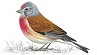
\includegraphics[]{Linnet_small.jpg}
       \end{figure} \linebreak
       The Software for symbolic Analysis of linear Electronic Circuits \linebreak
       Version 1.0 \linebreak
       User Guide
      }
\author{Peter Vranken}
\date{November 2014}

% Place chapter name and page number in the head of each page.
\pagestyle{headings}

\usepackage{hyperref}
\hypersetup{colorlinks, 
            citecolor=black,
            filecolor=black,
            linkcolor=black,
            urlcolor=black,
            bookmarksopen=false}


% The standard page filling is unsatisfyingly. Change it.
\textwidth160mm \textheight220mm
\addtolength{\oddsidemargin}{-10mm}
\addtolength{\evensidemargin}{-25mm}
\addtolength{\topmargin}{-10mm}

% TODO In the next major release use the following settings, which lead to
% a better balanced look of the printout. However, many layout corrections
% are needed: Tables, some figures and code fragments are to wide and at
% least one orphan has been found.
%\textwidth155mm \textheight210mm
%\addtolength{\oddsidemargin}{-8mm}
%\addtolength{\evensidemargin}{-22mm}
%\addtolength{\topmargin}{-5mm}

% Set the depth of the table of contents. The number plus 1 states the
% largest number of dot spearated section numbers appearing in the TOC.
% State e.g. 2 to get 1.2.3 as deepest nested section in the TOC.
\setcounter{tocdepth}{2}

% Technical terms like identifiers (object and function names) should be
% emphasized. Place them in the ident command. Similar for file names and
% short code snippets.
\newcommand{\ident}[1]{\textit{#1}}
\newcommand{\file}[1]{\textsf{#1}}
\newcommand{\code}[1]{\texttt{#1}}

\newcommand{\bs}{\textbackslash}

\begin{document}

% Document development: Turn preamble of actual text blocks on or off.
\ifthenelse{1=1}{
% Create titlepage
\maketitle

\bigskip
\begin{quote}
    Copyright \copyright{} 2014  Peter Vranken, mailto:Peter\_Vranken@Yahoo.de
    
    Permission is granted to copy, distribute and/or modify this document
    under the terms of the GNU Free Documentation License, Version 1.3
    or any later version published by the Free Software Foundation;
    with no Invariant Sections, no Front-Cover Texts, and no Back-Cover Texts.
    A copy of the license is included in the section entitled ``GNU
    Free Documentation License''.
\end{quote}
\bigskip


\tableofcontents \phantomsection
\listoffigures \phantomsection
\listoftables \phantomsection

%\chapter*{References}
\label{secDocReferences}

% A list of references to each quoted or mentioned external document. In
% your document you may write "please refer to \refL2Kurz2, page 23"
% instead of writing the title. Your document will then contain "please
% refer to [1], page 23".
% TODO Remove examples
\def\refExample{[1]}
% TODO Add a new reference here

\begin{longtable}[c]{|c|p{5.5cm}|p{8.0cm}|}

\hline
\label{tabDocReferences}
No. & Document & Explanation \\ \hline
% This hline makes the column titles a separate rectangular box, comment out to get just a
% line as separator.
%\hline
\endfirsthead

\hline
No. & Document & Explanation \\ \hline
% This hline makes the column titles a separate rectangular box, comment out to get just a
% line as separator.
%\hline
\endhead

\caption[]{References (continued on next page)}
\endfoot

\caption{References}
\endlastfoot

\hline

% Table entries start here.

% TODO Remove example
\refExample
  & notExistingExample.tex
  & This table entry is an example of how a reference to an external document could look
    like. Edit file chapReferences.tex to replace this entry with your required document
    references
\\ \hline

% TODO: Add a new document reference here
%\ref
%  & 
%  & 
%\\
%\hline

\end{longtable}
\chapter*{Abbreviations}
\label{secAbbreviations}

\begin{longtable}[c]{|l|l|}

\hline
\label{tabAbbrev}
Abbreviation & Explanation \\ \hline
% This hline makes the column titles a separate rectangular box, comment out to get just a
% line as separator.
%\hline
\endfirsthead

\hline
Abbreviation & Explanation \\ \hline
% This hline makes the column titles a separate rectangular box, comment out to get just a
% line as separator.
%\hline
\endhead

\caption[]{Abbreviations (continued on next page)}
\endfoot

\caption{Abbreviations}
\endlastfoot

\hline

% Table entries start here.
AC      & Alternating current                                  \\ 
CPU     & Central processing unit                              \\ 
DC      & Direct current                                       \\ 
DLL     & Dynamic link library                                 \\ 
GCC     & GNU compiler collection                              \\ 
GCD     & Greatest common divisor                              \\ 
GNU     & GNU is not UNIX                                      \\ 
LCM     & Least or lowest common multiple                      \\ 
LES     & Linear equation system                               \\ 
LHS     & Left-hand side (of an equation)                      \\ 
LTI     & Linear time-invariant (system)                       \\ 
MIMO    & Multiple input, multiple output (system)             \\ 
NPN     & N-type, p-type, n-type donated (transistor)          \\ 
op-amp  & Operational amplifier                                \\ 
R       & Resistor                                             \\ 
RHS     & Right-hand side (of an equation)                     \\ 
SIMO    & Single input, multiple output (system)               \\ 
SISO    & Single input, single output (system)                 \\ 
SW      & Software                                             \\ 
TBC     & To be checked                                        \\ 
TBD     & To be defined                                        \\ 
TODO    & To be done                                           \\
\hline

\end{longtable}
}

\chapter{Introduction}
\label{secIntro}

\linnet{} is an application to compute the transfer function of linear,
electronic circuits. The computation is done symbolically, not
numerically, and the result is a formula rather than a number or a series
of such. The found formula is the Laplace transform of the dependencies of
the voltages and currents in the circuit on the input voltages and
currents.


% Locally define a figure representation specific to the table.
{
\newcommand{\incTabFig}[2]{\includegraphics[width=#2]{#1}}

% This define is related to the specifics of the array package; see
% http://texwelt.de/wissen/fragen/3401/zentrieren-text-in-tabelle (as of
% July 25 2014) for more
\newcolumntype{M}[1]{>{\centering\arraybackslash}m{#1}}

\begin{table}[t]
\begin{center}
\begin{tabular}{|l|c|M{2cm}|}

\hline

% The column headers:
Device                               & ID          & Symbol                        \\
\hline

\hline

% Table entries start here.
%   The raisebox command is used to avoid a hiding overlap of the topmost
% figure with the header separating line.
\raisebox{0pt}[15pt][0pt]{Resistor}  & \code{R}    & \incTabFig{deviceR}{1.9cm}    \\ 
Conductance                          & \code{Y}    & \incTabFig{deviceY}{1.9cm}    \\
Capacitor                            & \code{C}    & \incTabFig{deviceC}{0.8cm}    \\ 
Inductivity                          & \code{L}    & \incTabFig{deviceL}{2cm}      \\ 
Ideal operational amplifier (op-amp) & \code{OP}   & \incTabFig{deviceOP}{1.3cm}   \\ 
Constant voltage source              & \code{U}    & \incTabFig{deviceU0}{1cm}     \\
Voltage controlled voltage source    & \code{U(U)} & \incTabFig{deviceU(u)}{1cm}   \\
Current controlled voltage source    & \code{U(I)} & \incTabFig{deviceU(i)}{1cm}   \\
Constant current soure               & \code{I}    & \incTabFig{deviceI0}{0.4cm}   \\
Voltage controlled current source    & \code{I(U)} & \incTabFig{deviceI(u)}{0.4cm} \\
Current controlled current source    & \code{I(I)} & \incTabFig{deviceI(i)}{0.4cm} \\
Current probe (wire)                 & \code{PI}   & \incTabFig{devicePI}{1.8cm}   \\ \hline
\end{tabular}
\caption{Supported linear devices}
\label{tabSupportedDevices}
\end{center}
\end{table}
} % End of local scope of \incTabFig

A linear electronic circuit is a combination of the supported basic
devices as listed in table \ref{tabSupportedDevices}. The circuit is input
to \linnet{}. The representation of the circuit is a list of devices with
connectivity information. The interconnections are expressed by references
to nodes, where a node is a point of the circuit, which normally at least
two devices are connected to. This leads to a simple formal syntax, the
circuit network list. This list can be created and maintained with a text
editor; there's no graphical interface for editing a circuit.

\begin{figure}
\centering
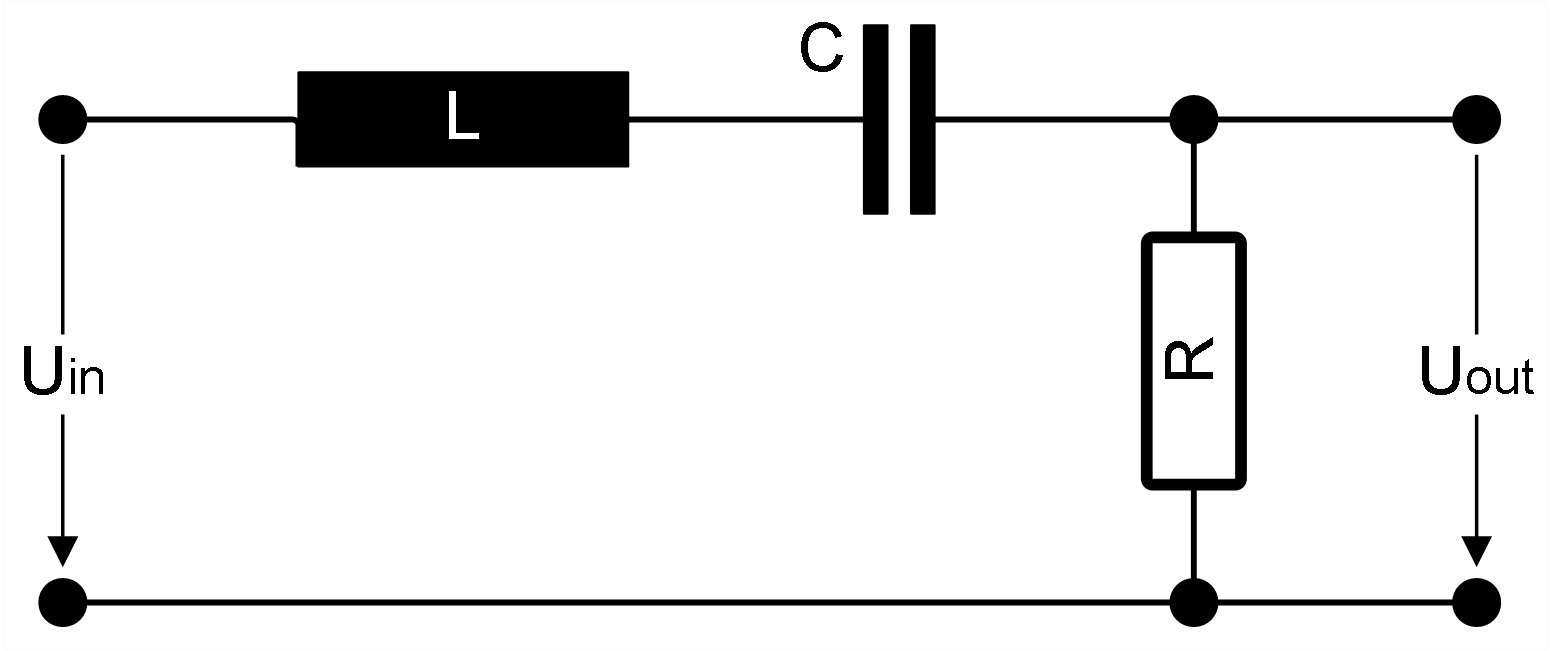
\includegraphics[width=5.29cm]{FirstIntroExample}
\caption{Simple example of a linear electronic circuit}
\label{figFirstIntroExample}
\end{figure}

The computed formulas are printed to the console and to the application
log file and can be used for further investigation or for publications or
didactic purpose.

To make the application somewhat more attractive it exports the computed
formulas as Octave or MATLAB script code, too. Numeric evaluation becomes
a simple one-line command in Octave. The formulas are exported as LTI
transfer function objects so that the complete set of analysis functions
from the Octave control toolbox can be applied just like that. This
reaches from simple transfer function plotting to stability analyses and
system response computation on arbitrary system input.

Please refer to figure \ref{figFirstIntroExample} as an example
of how \linnet{} works. This is a simple RLC element with a transfer
function of second order. It can be represented by the following circuit
netlist:
\begin{verbatim}
U Uin in  gnd
L L   in  K1
C C   K1  out
R R   out gnd
PLOT G U_out U_in
\end{verbatim}
Given this was put into file rlc.cnl, then we can run \linnet{}:
\begin{verbatim}
linNet -o rlc.cnl
\end{verbatim}
%\clearpage
and would yield the output:
\begin{verbatim}
User-defined result G (Bode plot):
The dependency of U_out on U_in:
  U_out(s) = N_U_out_U_in(s)/D_U_out_U_in(s) * U_in(s), with
    N_U_out_U_in(s) = R*C * s
    D_U_out_U_in(s) = L*C * s^2
                      +R*C * s
                      +1
\end{verbatim}

\begin{figure}
\centering
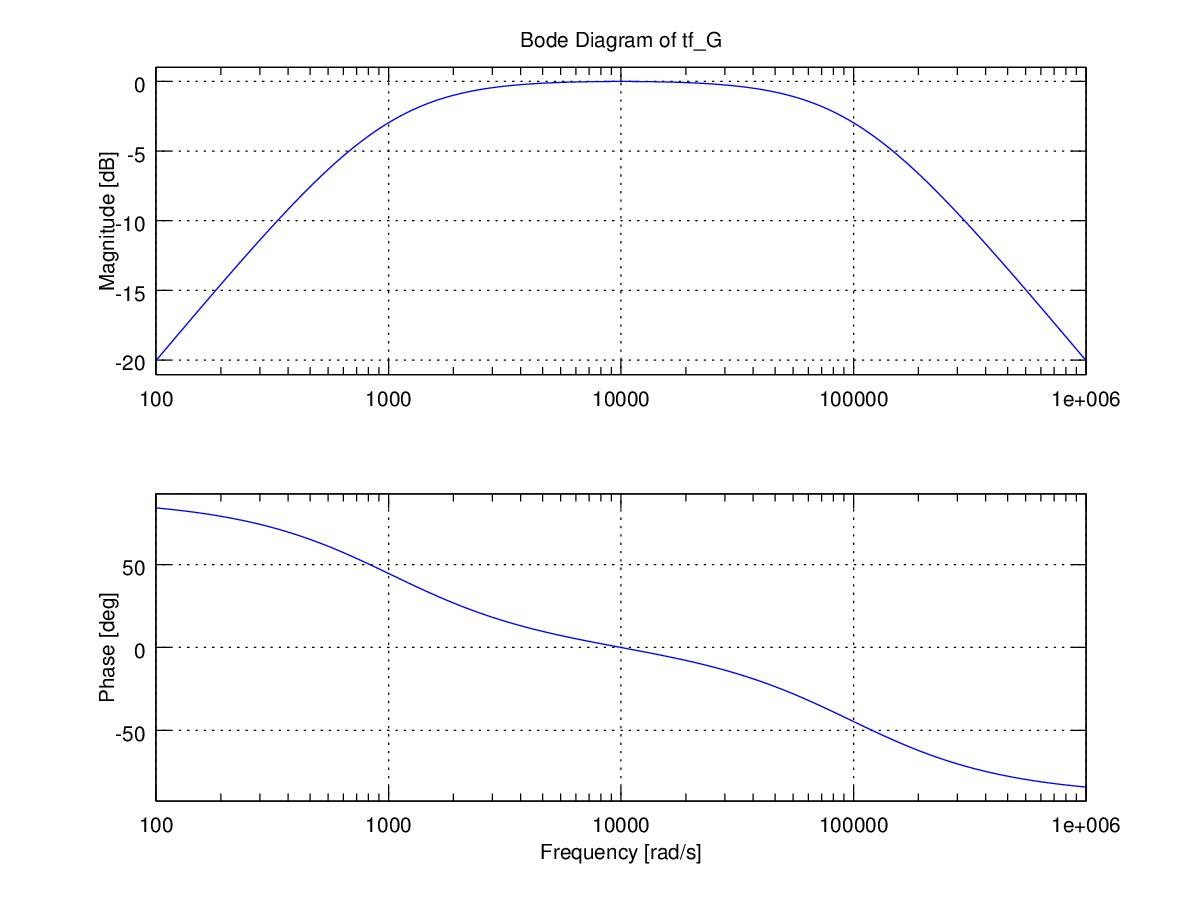
\includegraphics[width=0.7\textwidth]{FirstIntroExample_OctaveOutput}
\caption{Octave plot of transfer function of the system in figure
\ref{figFirstIntroExample}}
\label{figFirstIntroExample_OctaveOutput}
\end{figure}

Going to Octave and typing \code{G} to plot the transfer function (still
using default device values) gives us figure
\ref{figFirstIntroExample_OctaveOutput}. More plots or plots with altered
device values are a matter of single commands in Octave.

\linnet{} means ``linear network''. It founds on a symbolic solver for
linear equation systems. There's no way to model any non linear effects
like noise, voltage or current limits, non-linear distortions or switching
operations. All of these effects play an important role in real electronic
circuits and a good deal even uses these effects as their principle of
operation -- you won't find \linnet{} helpful for an investigation of
these kind of effects or circuits. There are many numeric circuit
simulation tools, which are capable to do this, in the first place the
popular open source tool SPICE with all its derivates. \linnet{} is
conceptually not a competitor of these tools, although it can behave a
tiny bit alike when using Octave as numeric post-processor. \linnet{} is
not the worse SPICE, \linnet{} is different.
\chapter{Installation}

A valid installation looks like this: The \linnet{} application is a
simple executable file plus a folder with resources for the Octave code
generator; this folder is called \file{private} and is located next to the
\linnet{} executable file, i.e. both are siblings in the same parent
directory. The environment variable \code{LINNET\_HOME} points to this
parent directory.

Accordingly, this is what you have to do to install \linnet{}: 

Create an empty folder, the installation directory, e.g.
\file{/ProgramFiles/linNet}. Copy the \linnet{} executable file into this
directory. Copy the folder \file{private} into this folder. Create a
persistent environment variable \code{LINNET\_HOME} and assign the path to
the installation directory, \code{/ProgramFiles/linNet} in our example.

The usual way to use \linnet{} is to run it from a shell window. You will
probably organize your input circuits in a folder or a set of such and
\code{cd} in your shell to this folder. To run \linnet{} in this scenario
in a convenient way it is useful to place a reference to the installation
directory in the system environment variable \code{PATH}. In our example
you'd append \code{:/ProgramFiles/linNet} (UNIX) and
\code{;\bs{}ProgramFiles\bs{}linNet} (Windows) to the current value of
this variable.

The definition of a shell command alias pointing to the \linnet{}
executable file can be a reasonable alternative to extending the
environment variable \code{PATH}.

If the environment variable is not set then \linnet{} makes an attempt to
find its resources via the path to itself. However, it depends on the
system, the shell in use and the way the command is typed, whether this
information is completely passed to the application or not. If it can't
find out where to find itself it'll refuse to generate Octave code as it
lacks the folder \file{private} with code templates.\footnote{There are
system specific functions which let an application find out, where its
executable file is located, e.g. \code{GetModuleFileName} for Windows, but
the use of such functions would make \linnet{} system dependent. This
price is much too high for an a bit simpler installation.} Not setting the
environment variable can be a safe option if you decide to run \linnet{}
solely from a shell window with an alias, which expands to the full,
absolute path of the executable.


\section{Mac OS}

Unfortunately, Macintosh users will have to compile \linnet{} from the
sources prior to use. At the moment no pre-built executables are available
for this system. Please refer to section \ref{secBuildingLinNet} on page
\pageref{secBuildingLinNet}.


\section{Linux}

The download of \linnet{} contains pre-build executable files for Linux
(in DEBUG and PRODUCTION compilation). The executable files are already
bundled with the resources folder \file{private} so that the installation
reduces to copying the build folder of choice to any location, preferably
\file{/usr/bin}, renaming the folder itself to \file{\linnet{}}, running
\code{chmod +x} to make the binary file executable and setting the
environment variable \code{LINNET\_HOME}; it would be set to
\file{/usr/\-bin/\-\linnet{}} if the suggested installation folder was
used. The chosen installation path should not contain blanks.

The Linux files have been built and run in a single environment only; this
was a Fedora 18 distribution. It can't be guaranteed that the binaries are
compatible with any other Linux derivate. Furthermore, no profound testing
has been done under Linux, only the few test cases from the distribution
have been run to prove that the expected program output is yielded. No
testing with Octave has been done under Linux.


\section{Windows}

\subsection{Pre-built executables}

The download of \linnet{} contains pre-build executable files for Windows.
A build for 32 and 64 Bit is contained, each as DEBUG or PRODUCTION
compilation. The executable files are already bundled with the resources
folder \file{private} so that the installation reduces to copying the
build folder of choice to any location, preferably
\file{c:\bs{}\-Program\-Files}, renaming the folder itself to
\file{\linnet{}} and setting the environment variable \code{LINNET\_HOME};
it would be set to \file{c:\bs{}\-Program\-Files\bs{}\-\linnet{}} if the
suggested installation folder was used. The chosen installation path
should not contain blanks.


\subsection{Required DLLs}

The build of \linnet{} has the executable file \file{linNet.exe} as only
product. This executable file is however not self-contained; the
application is linked against the compiler's C libraries, which in case of
the GNU compiler collection build on some Windows DLLs. These DLLs need to
be available in order to execute \linnet{}. Normally, this should always
be the case. In the rare case that such a library should be missing on
your system then the only way out will be to install the GCC port of MinGW
and to rebuild \linnet{}. If you can run the simplest \code{helloWorld}
application compiled with GCC then you should also be able to run
\linnet{}.

For a Windows 7 system and using the 32 Bit build the following list of
DLLs appeared to be loaded by \linnet{}. For different Windows releases or
for the 64 Bit build the list may vary:

\begin{verbatim}
c:\Windows\SYSTEM32\ntdll.dll
c:\Windows\SYSTEM32\wow64.dll
c:\Windows\SYSTEM32\wow64cpu.dll
c:\Windows\SYSTEM32\wow64win.dll
c:\Windows\SysWOW64\ntdll.dll
c:\Windows\syswow64\KERNELBASE.dll
c:\Windows\syswow64\kernel32.dll
c:\Windows\syswow64\msvcrt.dll
\end{verbatim}


\subsection{Start from Windows Explorer (file name association)}

If you want to start the computation of transfer functions directly from
the Windows Explorer then you can add a file class definition to the
Windows Registry. It'll extend the context menu entries of the Explorer
for circuit netlist files. With right-click on the file you can load the
netlist file into a text editor and by double-click you can run the
computation with \linnet{}. Please note, if starting \linnet{} this way
Windows will swallow all the program output and you will have to open the
log file after computation to find out if the computation was successful.

Here's a template for a Windows registry script to make an appropriate
file class definition:

% TODO Double-check appropriateness of \clearpage command after any change of chapter Installation
\clearpage
{\footnotesize
\begin{verbatim}
REGEDIT4

[HKEY_CLASSES_ROOT\.cnl]
@="FileClass_cnl"

[HKEY_CLASSES_ROOT\.ckt]
@="FileClass_cnl"

[HKEY_CLASSES_ROOT\FileClass_cnl]
@="linNet Circuit Netlist"

[HKEY_CLASSES_ROOT\FileClass_cnl\shell]
@="Compute"

[HKEY_CLASSES_ROOT\FileClass_cnl\DefaultIcon]
@="c:\\ProgramFiles\\linNet\\linNet.exe,1"

[HKEY_CLASSES_ROOT\FileClass_cnl\shell\Edit]
@="&Edit"
[HKEY_CLASSES_ROOT\FileClass_cnl\shell\Edit\command]
@="c:\\ProgramFiles\\emacs-24.0.92\\bin\\emacsclient.exe -n \"%1\""

[HKEY_CLASSES_ROOT\FileClass_cnl\shell\Compute]
@="Run linNet"
[HKEY_CLASSES_ROOT\FileClass_cnl\shell\Compute\command]
@="c:\\ProgramFiles\\linNet\\linNet.exe -l -c -s -o \"%1\" %*"
\end{verbatim}
} % End of decreased script size for the listing

Copy this code into a text file. Save it using a file name with extension
\file{.reg}, e.g. \file{fileClassCnl.reg}.

Please note, that you will have to modify the proposed code as it uses
absolute paths to the installed applications; replace these paths with
your system's paths. Furthermore, the text editor for editing the circuit
netlists is just a suggestion; you will probably replace the reference to
Emacs with a reference to your favorite text editor.

After customization, double-click this file or run it from a shell window.
If your system has no file name association for \file{*.reg} files then
you need to import it explicitly using a command like \code{regedit.exe
fileClassCnl.reg}. In either case you will need local administrator rights
to complete.
\chapter{The Command Line Interface}

\linnet{} is a simple console application. It is fully controlled by the
command line arguments and all its output is text based, either printed
to the console or written into the output files.

All interaction with \linnet{} is done from a shell window. From such a
window type \code{linNet --help} to get a short reminder on the available
command line options.

The command line may contain program options and the names of the input
files, which are always circuit netlist files. The order of options and
file names doesn't matter but usually all the file names are placed behind
all the options. If a file name could be mixed up with an option then the
double hyphen (\code{--}) can be placed on the command line: All remaining
command line arguments are considered file names regardless of how they
look like.

Circuit netlist files are named \code{*.cnl} by convention but they may
follow any other name pattern. Only the file name extension \code{*.ckt}
is reserved and must not be used.

All the information that impacts the conducted computations is placed in
the circuit netlist files; the program options only affect the generated
output. The verbositiy of the console output can be controlled, a log file
can be created and the output for Octave is an option only. The command
line arguments in detail:
\begin{itemize}
  \item \emph{-h, --help}
    \linnet{} prints a short help text and terminates again. The return
    value to the shell is 0. Can be combined with \code{-r}
  \item \emph{-r, --version}
    \linnet{} prints the software revision and terminates again. The
    return value to the shell is 0. Can be combined with \code{-h}
  \item \emph{-v LEVEL, --verbosity=LEVEL}
    The verbosity LEVEL of the application; LEVEL is an enumeration value.
    It doesn't matter whether it is written in upper or lower case
    characters. The blank between \mbox{-v} and LEVEL is optional. LEVEL
    applies in the same way to the console output and the application log
    file. In general, the same information is written to both of these
    streams. LEVEL is one out of:
    \begin{itemize}
      \item \code{DEBUG}: A lot of internal information about the progress
        of the computation is printed to the console. Among more, the
        linear equation system is printed prior to and after running the
        solver. For complex circuits this can mean many thousand lines of
        output or much time to wait.
        
        A strong recommendation is to use this level of verbosity solely
        in conjunction with the other option \code{-s}, which suppresses
        all console output. (Writing to the log file only is times faster
        then writing to the console)
        
      \item \code{INFO}: Some progress information is printed. Among more,
        the algebraic solution of the linear equation system is printed,
        which can still mean bulky output. Use this level of verbosity
        with care 
        
      \item \code{RESULT}: This is the default level of verbosity. All
        final results are printed, i.e. the requested variables in the
        frequency domain.
        
        Additionally, if a concise log format is chosen (see \code{-f}),
        which doesn't have time stamps, then \code{RESULT} will also print
        some timing information.
        
      \item \code{WARN}: The warnings are printed. Computation results can
        be found only exported as Octave code (see~\code{-o})
        
      \item \code{ERROR} The error messages are printed. Computation
        results can be found only exported as Octave code (see~\code{-o})
        
      \item \code{FATAL}: Only the fatal error messages are printed. Fatal
        errors (as opposed to the ``normal'' errors) are those, which lead
        to immediate (but still controlled) program termination; the
        out-of-memory error is a prominent example. Computation results --
        if any -- can be found only exported as Octave code (see~\code{-o})
    \end{itemize}
    Default is \code{RESULT}. Any verbosity level includes all output of
    the less verbose levels.

  \item \emph{-f FORMAT, --format-of-log-entry=FORMAT}
    Log entry format. FORMAT is an enumeration value. It doesn't matter
    whether it is written in upper or lower case characters. The blank
    between -f and FORMAT is optional. FORMAT is one out of:
    \begin{itemize}
      \item \code{raw}: Only the pure message text is printed to the
        console and the log file
        
      \item \code{short}: Each message is preceeded by a short line
        header, which contains the consumed CPU time and the severeness of
        the message
        
      \item \code{long}: Each message is preceeded by a line header, which
        contains a time stamp, the consumed CPU time and the severeness of
        the message.
    \end{itemize}
    The default format is \code{long}

  \item \emph{-s, --silent}
    Silent operation, only a greeting is emitted. Do not write progress
    information to the console, only write into the log file. To avoid
    useless runs of the application it is not allowed to choose silent
    operation if no log file is in use (see~\code{-l})
    
  \item \emph{-l[FILENAME], --log-file-name[=FILENAME]}
    This option enables the use of a log file and controls its name. No
    log file is opened if this option is not used.
    
    You may state the name of the log file but normally you won't: If the
    option is used without argument \code{FILENAME} then an appropriate
    file name is chosen by the application. It is derived from the name of
    the circuit netlist if a single input file is given and otherwise a
    generic name is chosen.
    
    There's a constraint: Either using a log file is specified with
    \code~{-l} or~\code{-s} (or \code{--silent}) is not given 
    
  \item \emph{-c, --clear-log-file}
    Clear the log file at the beginning of operation. Default is to append
    to a possibly already existing log file
    
  \item \emph{-o[DIRNAME], --Octave-output-directory[=DIRNAME]}
    This option enables the generation of Octave script code and controls
    the location. No Octave code is generated if this option is not used.

    Octave code generated from a circuit netlist will be placed into a
    folder whose name is derived from the netlist file. As many output
    folders will be created as input files are given. All of these folders
    will be placed into a common parent directory and this directory is
    designated by \code{DIRNAME}. If \code{DIRNAME} is omitted then the
    current working directory is used as common parent directory

  \item \emph{-i, --do-not-copy-common-Octave-code}
    The generated Octave code builds on some common scripts, which are
    normally copied into each of the netlist related output folders. This
    way the generated code will run just like that in Octave, without the
    need of manipulating Octave's search path. If you dislike the over and
    over copied, always identical files you can consider to install them
    once in your Octave environment and to let them no longer be produced
    by \linnet{}.
    
    If you give this option then copying the common files into each output
    folder is simply not done.
    
    This switch is relevant only if \code{-o} is also given

\end{itemize}

If the command line parser detects a problem then it tends to print the
help text for convenience. This is done into stdout. The concrete error
report is however printed into stderr. It depends on your shell in which
fashion these two text streams are separated (or interchanged). Carefully
look for the actual error message; if you are lucky it's presented in a
different color.

If \linnet{} is integrated in a scripting environment then its return
value may matter. Normally, \linnet{} returns 0 to the calling shell. If
the command line parser recognizes an error or if any input file can't be
opened or if it causes a computational error then \linnet{} returns -1.
The error cause cannot be concluded from the return value, the log file
needs to be inspected to find out.



\chapter{The Syntax of the Input File}

Most of the functionality of \linnet{} is controlled from the input file.
The main part of the input file is the circuit netlist: Each line of code
defines a single electronic device with the network nodes it is connected
to. The number of nodes varies from two to four and depends on the kind of
device. Nodes are defined implicitly the first time they are referenced by
a device definition.

The remaining parts of the file are used to specify the wanted results.
This part of the file may stay empty, in which case all unknown quantities
are computed.


\section{Basic syntax elements}

A netlist file may of course be well-documented. You can use C/C++ style
comments anywhere. Nested comments are not supported.

A semicolon is treated like an end of line character. Line concatenation
can be achieved with a backslash as very last character of a line, as in
the language C.

All elements of the formal syntax of the input file are treated case
sensitive.

The names of devices, nodes, user-defined voltages and results are defined
as identifiers in most computer languages. They begin with a letter or
underscore and can continue with any number of the same or decimal digits.
This particularly disables integer numbers to become node designations as
it is common in SPICE netlists.

The names of knowns and unknowns are internally derived from the device
and node names and are in turn ``identifiers''. 


\begin{longtable}{|c|c|c|}

\hline
\label{tabExponentSuffixes}
% The column headers (first page):
Suffix & Meaning & Value \\ \hline
% This hline makes the column titles a separate rectangular box, comment out to get just a
% line as separator.
%\hline
\endfirsthead

\hline
% The column headers (other pages):
Suffix & Meaning & Value \\ \hline
% This hline makes the column titles a separate rectangular box, comment out to get just a
% line as separator.
%\hline
\endhead

\hline
\caption{Suffixes for exponents in floating point literals (continued on next page)} 
\endfoot

\hline
\caption{Suffixes for exponents in floating point literals}
\endlastfoot

\hline

% Table entries start here.
\code{y} & yocto & \raisebox{0pt}[10pt][0pt]{$10^{-24}$} \\
\code{z} & zepto & \raisebox{0pt}[10pt][0pt]{$10^{-21}$} \\ 
\code{a} & atto  & \raisebox{0pt}[10pt][0pt]{$10^{-18}$} \\ 
\code{f} & femto & \raisebox{0pt}[10pt][0pt]{$10^{-15}$} \\ 
\code{p} & pico  & \raisebox{0pt}[10pt][0pt]{$10^{-12}$} \\ 
\code{n} & nano  & \raisebox{0pt}[10pt][0pt]{$10^{-9}$}  \\ 
\code{u} & micro & \raisebox{0pt}[10pt][0pt]{$10^{-6}$}  \\ 
\code{m} & milli & \raisebox{0pt}[10pt][0pt]{$10^{-3}$}  \\ 
\code{c} & centi & \raisebox{0pt}[10pt][0pt]{$10^{-2}$}  \\ 
\code{d} & deci  & \raisebox{0pt}[10pt][0pt]{$10^{-1}$}  \\ 
\code{D} & deka  & \raisebox{0pt}[10pt][0pt]{$10^{1}$}   \\ 
\code{h} & hecto & \raisebox{0pt}[10pt][0pt]{$10^{2}$}   \\ 
\code{k} & kilo  & \raisebox{0pt}[10pt][0pt]{$10^{3}$}   \\ 
\code{M} & mega  & \raisebox{0pt}[10pt][0pt]{$10^{6}$}   \\ 
\code{G} & giga  & \raisebox{0pt}[10pt][0pt]{$10^{9}$}   \\ 
\code{T} & tera  & \raisebox{0pt}[10pt][0pt]{$10^{12}$}  \\ 
\code{P} & peta  & \raisebox{0pt}[10pt][0pt]{$10^{15}$}  \\ 
\code{X}\footnote{According to
http://searchstorage.techtarget.com/definition/Kilo-mega-giga-tera-peta-and-all-that,
as of Feb 9, 2014, exa should be abbreviated with \code{E}. This is
ambiguous with the traditional form of an exponent. \code{1E+2} could be
either $10^{18}+2$ or $100$. We use \code{X} instead.}
         & exa   & \raisebox{0pt}[10pt][0pt]{$10^{18}$}  \\
\code{Z} & zetta & \raisebox{0pt}[10pt][0pt]{$10^{21}$}  \\ 
\code{Y} & yotta & \raisebox{0pt}[10pt][0pt]{$10^{24}$}  \\ 

\end{longtable}

Numbers are either decimal integer literals as known from the language C
or floating point numbers, depending on the context. Floating point numbers
can be written as known from the language C. For convenience, the exponent
may be abbreviated by a suffix character; just type this single character
instead of the conventional exponent expression, write for example
\code{5.6k} instead of \code{5.6e3}. Careful, the suffixes are case
sensitive, too, \code{5.6K} would yield a syntax error. The supported
suffixes are listed in table \ref{tabExponentSuffixes}

More details on the syntax definition can be found in file
\file{parser-cnl-bnf.txt}. The syntax is presented in commented
Backus-Naur form. The file is printed in appendix \ref{secBNFOfCnl} on
page \pageref{secBNFOfCnl} of this document and it is part of the
\linnet{} sources.


\section{The actual netlist}

The main part of the input file is a list of device definitions. Each
definition is placed on a new line or a semicolon is used to seperate two
definitions on the same line. A device definition starts with the device
type that indicates the kind of device. Table \ref{tabSupportedDevices} on
page \pageref{tabSupportedDevices} gives an overview on the available
devices. The type identifier from table column ID is used as first token
of a device definition in the netlist file.

The name of the device follows after some white space. All names need to
be unique in order to avoid ambiguities in the result presentation. Then
the names of the nodes the device is connected to follow up as a blank
separated list. The kind of device determines the required number of
nodes, see below.\footnote{The syntax format defines the nodes by position
in the line only. If a node name is missing in the line the next token
will be taken as this node and a missleading error message can result.
Which might be particularly confusing if it is not the last node, which
has been omitted.} There's no explicit definition of nodes; a node is
defined implicitly when referencing it in a device definition the very
first time. This doesn't hold for the voltage sensing inputs of a voltage
controlled source (the third and forth node in the device definition).
They are pure references to a pair of nodes, which need to be defined
elsewhere. Normally the parser doesn't support forward references but here
we have one of the few exceptions; the actual definition of the the source
controlling nodes may be made with a later device definition:

% Wrap text after line 87 in the verbatiom section.
\begin{verbatim}
/* This system has the input impedance Ri and an output voltage, which is the k-fold
   of the input voltage. */
U(U) k out gnd in gnd // Voltage controlled voltage source k is defined. Nodes out and
                      // gnd are implicitly defined. Nodes in and gnd are referenced;
                      // node in is not yet defined, we have a forward reference.
R Ri in gnd           // Resistor Ri is defined. Node in is implicitly defined and the
                      // above forward reference can be resolved.
U Ui in gnd           // The input voltage is modeled by a constant voltage source
\end{verbatim}

An optional blank separated device relation may follow the node
references. The device relation supports numeric post-processing and
simplifications of the final result. The simplest form of a device
relation is the assignment of a numeric value. Such an assignment has no
impact on \linnet's computation, it is solely passed on to Octave for
numeric evaluation via the generated script code. An example would be

\begin{verbatim}
R R1 k0 k1 R1=5.6k
\end{verbatim}

\noindent
which defines the resistor \code{R1}, connects it to the two nodes
\code{k0} and \code{k1} and assigns it a value of 5600\,$\Omega$. The
generated Octave script code will initialize the variable \code{R1} with
the numeric value $5600.0$. All variables which no user-defined values are
found for in the netlist file will get fixed standard values as initial
values in the generated Octave script code. The standard values are
defined such that the characteristic time constants of the circuit are
probably in the audio frequency range. Changing these standard values to
more appropriate values can then be done on the Octave command line. The
hardcoded standard values of all affected devices are listed in table
\ref{tabDeviceStdValues} on page \pageref{tabDeviceStdValues}.

More important than value assignments are relations between devices of
same kind. The most simple case would be the identity of the values of two
devices, e.g. \code{R1=R2}. Many circuits depend on such a relation; a
voltage divider with two identical resistors is for example often used to
pin the input voltage of an op-amp to half the operational voltage. If a
pair of devices has a fixed value relation as a principle of operation of
the circuit then this should be expressed in the netlist. The knowledge
about value relations enables \linnet{} to perform according
simplifications of the final result, it would e.g. simplify a term like
$R_1 R_2 C$ to ${R_2}^2 C$ in the previous example. An impressive example
of such simplifications is found as \file{octagon.cnl} in the set of test
cases in the source code distribution of \linnet{}.

Device relations can be made recursively. The netlist\footnote{The tokens
\code{DEF} and \code{RES} are explained below in section
\ref{secResultSpec}.}

\begin{verbatim}
U Uin in gnd
R R1 in k1
R R2 k1 k2  R2=R1
R R3 k2 k3  R3=R2
R R4 k3 gnd R4=R3
DEF Uout k3 gnd
RES VDiv Uout
\end{verbatim}

\noindent
defines a voltage divider into four identical voltages. Due to the given
relations, the result formula will no longer contain any device symbol,
but simply states $\frac{1}{4}U_{in}$ for the output voltage.

Device relations can use rational ratios. We could achieve the same result
with the following netlist:

\begin{verbatim}
U Uin in gnd
R R1 in k1
R R2 k1 gnd R2=1/3*R1
DEF Uout k1 gnd
RES VDiv Uout
\end{verbatim}

\linnet{} claims to be a symbolic not a numeric program. Such a software
is expected to produce exact, error free results only. Permitting rational
ratios between two devices introduces some numeric calculations but these
can still be carried out error free -- with the exception of overflows.
Making intensive use of such relations will easily produce such an
overflow. \linnet{} will recognize the overflow but not perform any
approximative computations. You either get an accurate result or no result
(but the error message). The danger of an overflow rises if you use ratios
of large numbers that are prime to each other or if you use recursive
device ratios as in the next example, which again has the same output
voltage:

\begin{verbatim}
U Uin in gnd
R R1 in k1
R R2 k1 k2  R2=(7/8)*R1
R R3 k2 gnd R3=(5/7)*R2
DEF Uout k2 gnd
RES VDiv Uout
\end{verbatim}

\noindent
To reduce the danger of overflows due to careless use of the rational
ratios the values of numerator and denominator of the ratios are limited
to the range $1..999$. Null and negative ratios are generally not
permitted. Negative ratios can be useful with controlled sources; if so
the appropriate sign has to be chosen by the polarity of either the source
or the control voltage or current.

Device relations must not use forward references. 

The definition of the device is closed with either a newline character or
semicolon. Newline characters must not be used to spread a device
definition over several lines but several device definitions can share the
same line if the semicolon is used.


\subsection{Which nodes to connect to}

% The schematics used as examples in this section are placed at the
% begining of the source code section in order to give LaTeX room to
% distribute them over all pages.

% Sample circuit: Current probe and current controlled current source
{
% This define is related to the specifics of the array package; see
% http://texwelt.de/wissen/fragen/3401/zentrieren-text-in-tabelle (as of
% July 25 2014) for more
\newcolumntype{M}[1]{>{\centering\arraybackslash}m{#1}}

\begin{figure}[t]
\begin{center}
% The standard total width of 11cm leads here to an ugly gap between
% netlist and schematic. We reduce it by 1cm.
\begin{tabular}{M{5.42cm}M{4.58cm}}
\verbatiminput{SimpleT.cnl}
&
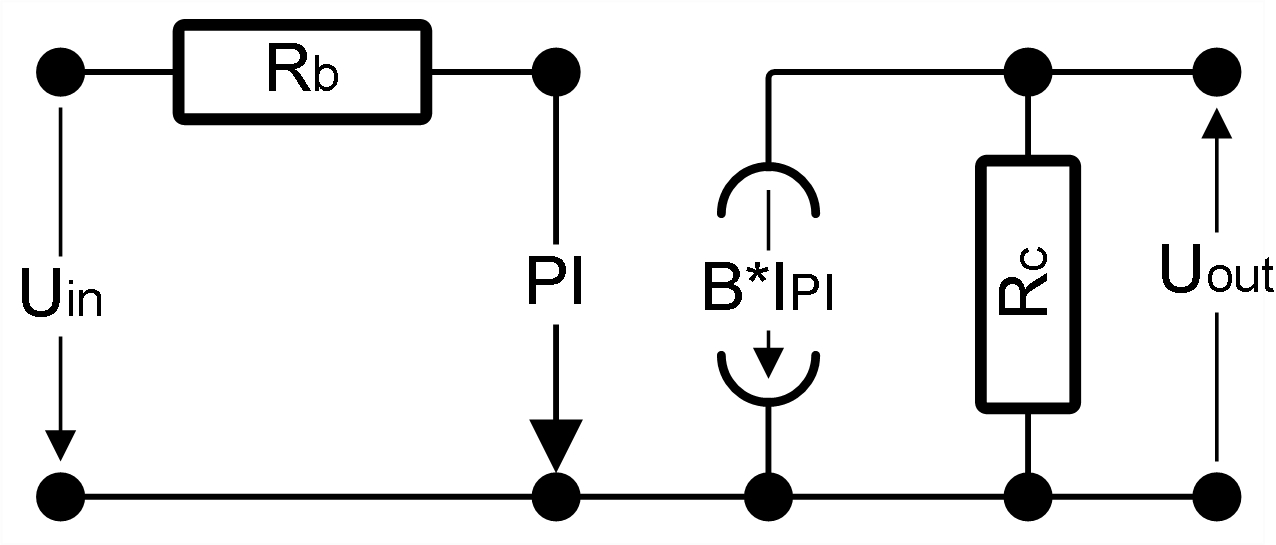
\includegraphics[width=4.58cm]{SimpleT}
\\

\end{tabular}
\caption{A simple bipolar transistor simulation}
\label{figSimpleT}
\end{center}
\end{figure}
} % End of sample circuit: Current probe and current controlled current source

% Sample circuit: The non inverting op-amp.
{
% This define is related to the specifics of the array package; see
% http://texwelt.de/wissen/fragen/3401/zentrieren-text-in-tabelle (as of
% July 25 2014) for more
\newcolumntype{M}[1]{>{\centering\arraybackslash}m{#1}}

\begin{figure}[b]
\begin{center}
\begin{tabular}{M{5.84cm}M{5.16cm}}
\verbatiminput{NonInvertingOP.cnl}
&
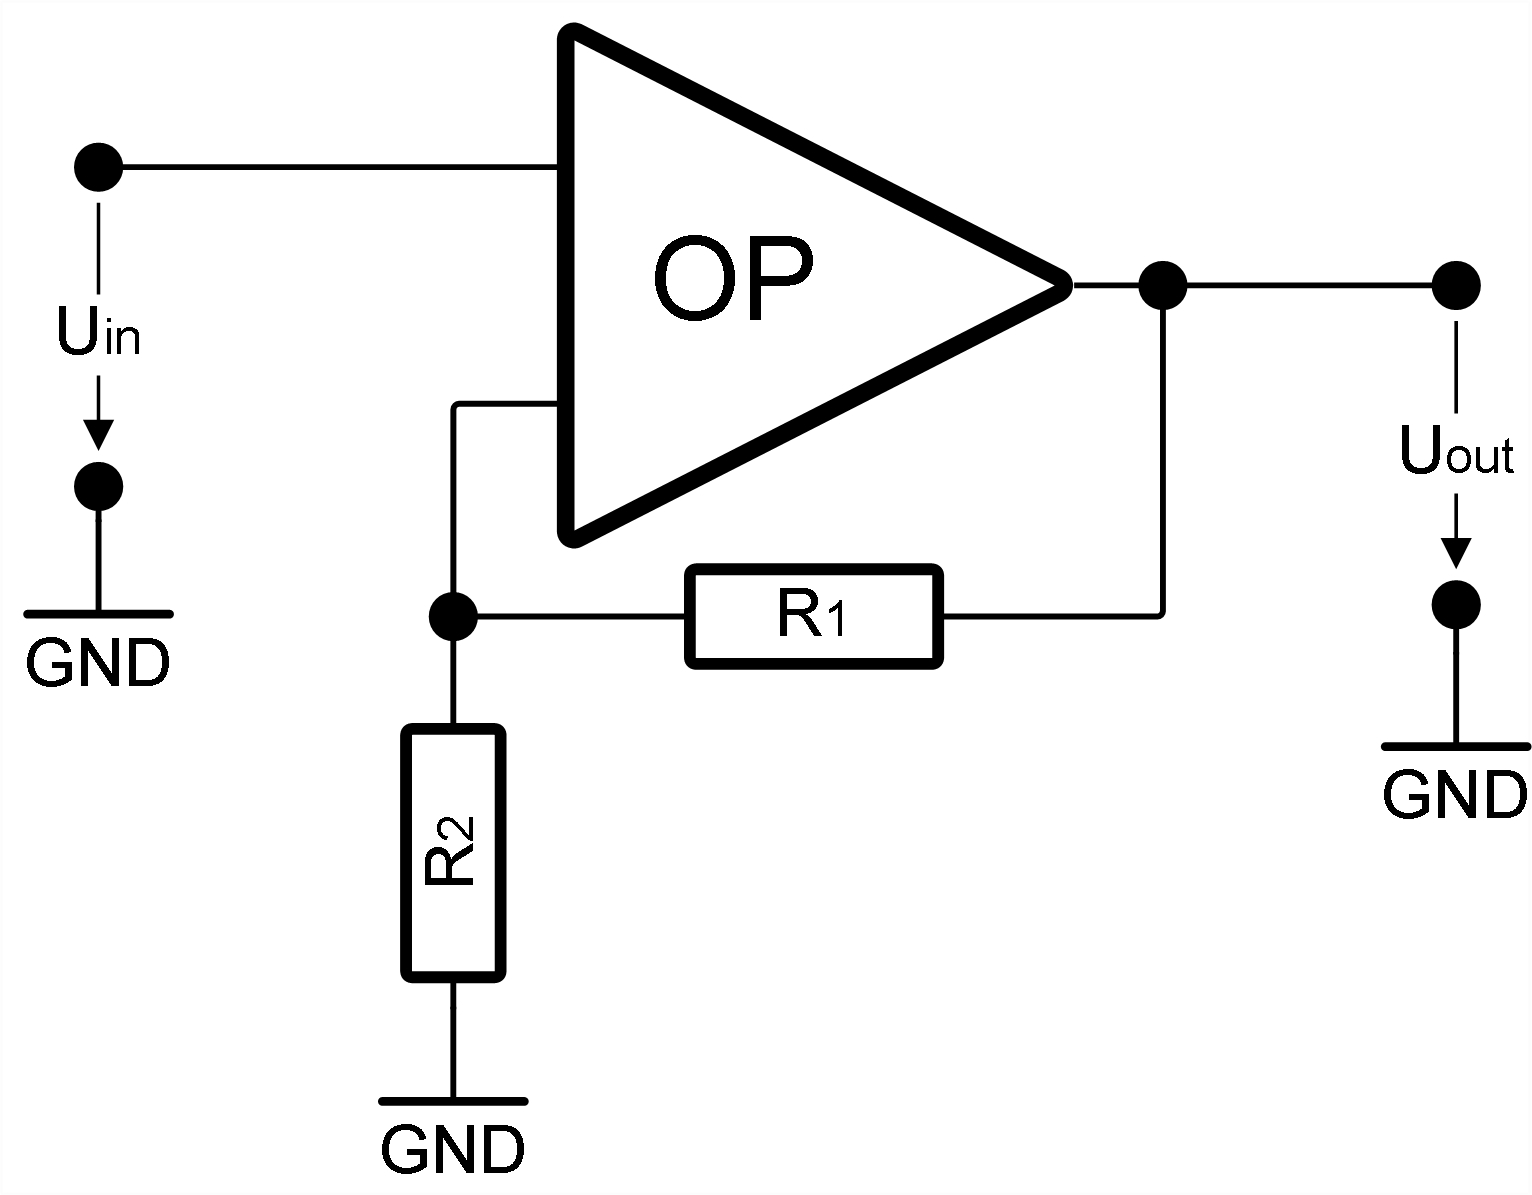
\includegraphics[width=5.16cm]{NonInvertingOP}
\\

\end{tabular}
\caption{Non inverting op-amp}
\label{figNonInvOp}
\end{center}
\end{figure}
} % End of sample circuit: The non inverting op-amp.

% Sample circuit: Model of inverting op-amp.
{
% This define is related to the specifics of the array package; see
% http://texwelt.de/wissen/fragen/3401/zentrieren-text-in-tabelle (as of
% July 25 2014) for more
\newcolumntype{M}[1]{>{\centering\arraybackslash}m{#1}}

\begin{figure}[t]
\begin{center}
\begin{tabular}{M{6.65cm}M{4.35cm}}
\verbatiminput{ModelOfOP.cnl}
&
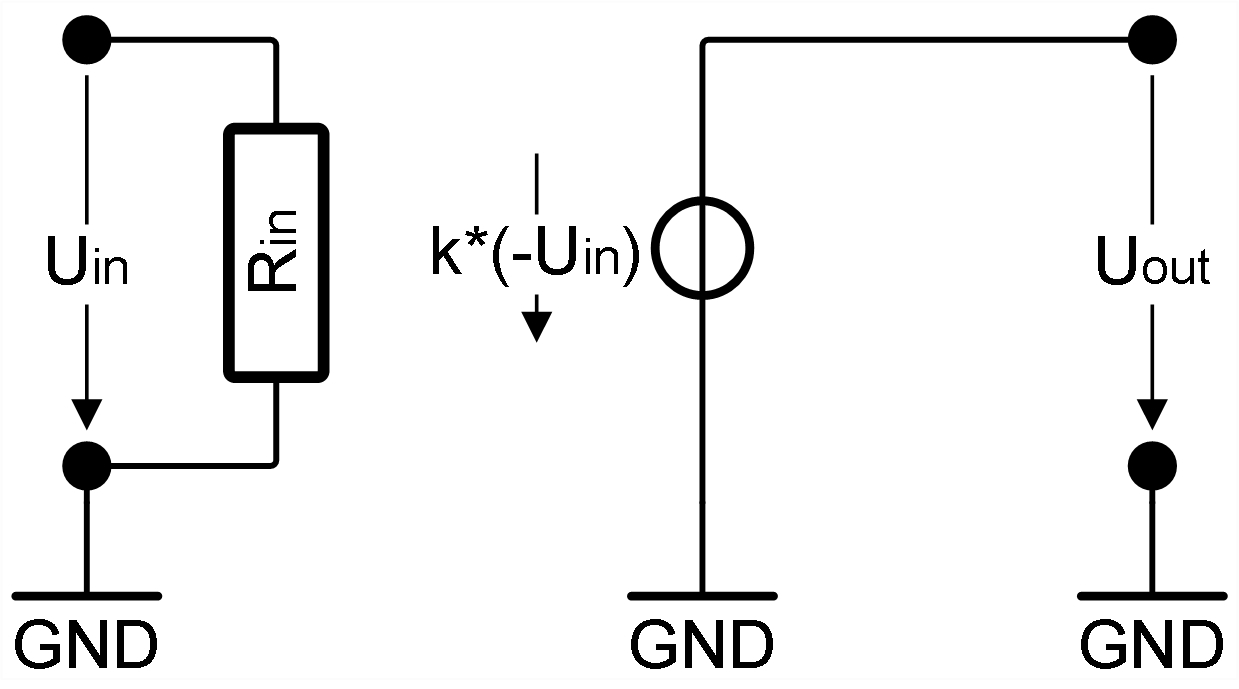
\includegraphics[width=4.35cm]{ModelOfOP}
\\

\end{tabular}
\caption{Model of the inverting op-amp}
\label{figModelOfOP}
\end{center}
\end{figure}
} % End of sample circuit: Model of inverting op-amp.

% Sample circuit: Current controlled voltage source
{
% This define is related to the specifics of the array package; see
% http://texwelt.de/wissen/fragen/3401/zentrieren-text-in-tabelle (as of
% July 25 2014) for more
\newcolumntype{M}[1]{>{\centering\arraybackslash}m{#1}}

\begin{figure}[b]
\begin{center}
\begin{tabular}{M{5.73cm}M{5.27cm}}
\verbatiminput{I2UConverter_U(i).cnl}
&
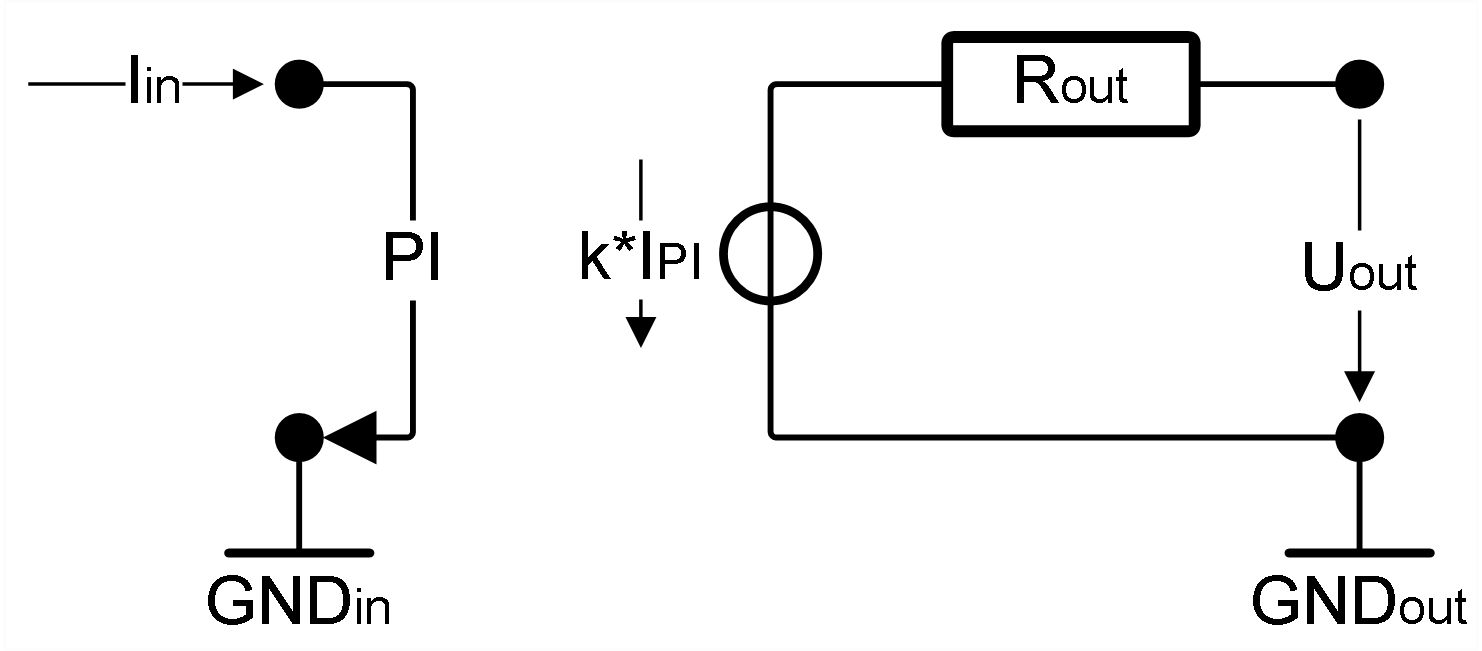
\includegraphics[width=5.27cm]{I2UConverter_U(i)}
\\

\end{tabular}
\caption{Current to voltage converter using a current controlled voltage source; $R_i=0$,
$R_o=R_{out}$}
\label{figI2UConverterUsingUByI}
\end{center}
\end{figure}
} % End of sample circuit: Current controlled voltage source

% Sample circuit: Voltage controlled current source
{
% This define is related to the specifics of the array package; see
% http://texwelt.de/wissen/fragen/3401/zentrieren-text-in-tabelle (as of
% July 25 2014) for more
\newcolumntype{M}[1]{>{\centering\arraybackslash}m{#1}}

\begin{figure}[tb]
\begin{center}
\begin{tabular}{M{5.62cm}M{5.38cm}}
\verbatiminput{I2UConverter_I(u).cnl}
&
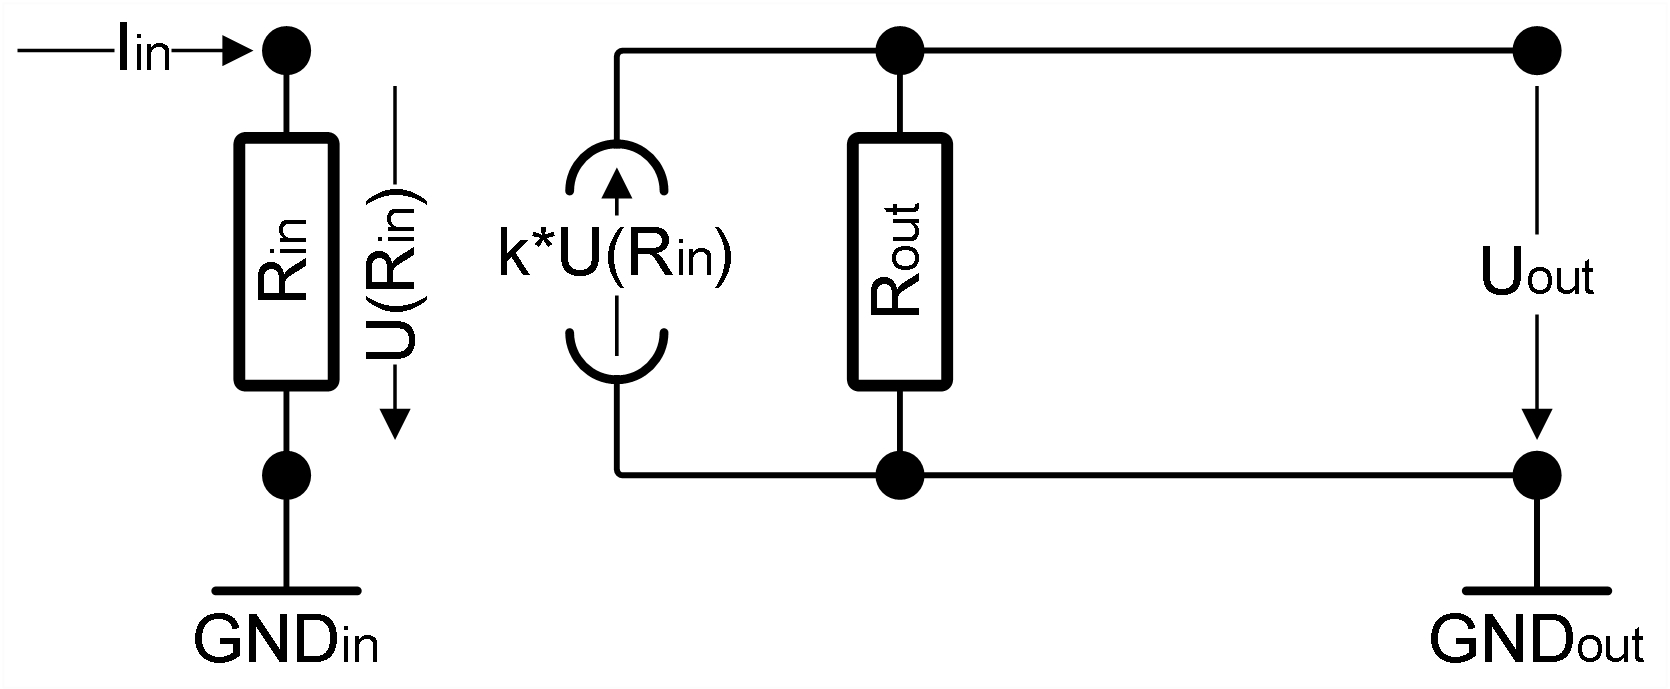
\includegraphics[width=5.38cm]{I2UConverter_I(u)}
\\

\end{tabular}
\caption{Current to voltage converter using a voltage controlled current source; $R_i=R_{in}$,
$R_o=R_{out}$}
\label{figI2UConverterUsingIByU}
\end{center}
\end{figure}
} % End of sample circuit: Voltage controlled current source

% End of list of figures of sample schematics used in the section.


\subsubsection{Passive device \code{R}, \code{Y}, \code{L}, \code{C}}

The passive devices resistor \code{R}, conductance \code{Y}, inductivity
\code{L} and capacitor \code{C} have two connectors and they are
independent of the chosen polarity. Just connect them by referencing two
nodes.

An example netlist can be found in section \ref{secIntro}; please refer to figure
\ref{figFirstIntroExample}, too.


\subsubsection{Constant voltage source \code{U}}

The constant voltage source \code{U} has two connectors. The plus and
minus pole of the source are the first and second referenced node,
respectively. The polarity is defined such that the first and second
referenced node designate the start and end of the arrow in the symbol of
the source (or voltage).

The given voltage of the source is an independent variable to the
computation but not considered a settable physical value; no value
assignment or device relation can be made in the definition of a constant
voltage source. The constant voltage appears as a variable in the
results.

At least one constant source, either voltage or current, needs to be
present in a computable netlist.

An example netlist is shown in figure \ref{figSimpleT}.


\subsubsection{Constant current source \code{I}}

The constant current source \code{I} has two connectors. The polarity is
defined such that the first and second referenced node designate the start
and end of the arrow in the symbol of the source: The current is flowing
into the network through the second referenced node and flowing back into
the source from the first referenced node.

The given current of the source is an independent variable to the
computation but not considered a settable physical value; no value
assignment or device relation can be made in the definition of a constant
current source. The constant current appears as a variable in the results.

At least one constant source, either voltage or current, needs to be
present in a computable netlist.

An example netlist is shown in figure \ref{figI2UConverterUsingUByI}.


\subsubsection{Current probe \code{PI}}
\label{secSyntaxCurrentProbe}

The current probe \code{PI} has two connectors and can be connected in
series with any other device to measure the current flowing through the
device. The sensed current becomes a new unknown, which can be
referenced in user-defined results.

The polarity of the measured current is defined such that the sensed
current is flowing into the probe from the first referenced node and
flowing back into the network through the second node.

A current probe is assumed an ideal wire. It has no physical value(s); no
value assignment or device relation can be made in the definition of a
current probe.

An example netlist is shown in figure \ref{figSimpleT}.


\subsubsection{Operational amplifier \code{OP}}

An operational amplifier \code{OP} has three connectors; connect them by
referencing three nodes.

The first two referenced nodes are the inputs. Different to real
circuits no distinction needs to be made between the two inputs; there's
no inverted or non inverted input. The computation needs to assume the linear
operation -- everytking else is out of scope of \linnet{} -- and in this
sense the connection is always made correct.

The third referenced node is the output of the op-amp.

Please note that the ground node needs to be explicitly defined if an
op-amp is used; see section \ref{secGndNode} for details.

An op-amp is assumed ideal. It has no output voltage or frequency limits
and hence no physical value(s); no value assignment or device relation can
be made in the definition of an op-amp.

An example netlist is shown in figure \ref{figNonInvOp}.


\subsubsection{Voltage controlled voltage source \code{U(U)}}

The voltage controlled voltage source \code{U(U)} has four connectors. The
actual source has two; these are the first two nodes referenced in the
device definition. The first node designates the positive pole of the
source, the second one the negative pole. First and second referenced
node designate start and end of the voltage defining arrow in the
schematic.

The control voltage is defined by the voltage potential difference between
node three and four, in this order. The third and forth referenced node
designate start and end of the voltage arrow in the schematic,
respectively.

An example netlist is shown in figure \ref{figModelOfOP}. Please note,
that the control voltage in this example is defined inverse to the input
voltage in order to model the inverting op-amp.


\subsubsection{Current controlled voltage source \code{U(I)}}

The current controlled voltage source \code{U(I)} has two connectors. The
first referenced node designates the positive pole of the source, the
second one the negative pole. First and second referenced
node designate start and end of the voltage defining arrow in the
schematic.

The control current is specified by a reference to a current probe. The
current probe is another, previously defined device (forward references
are not supported), which behaves like an ideal wire. The current through
this wire times the device constant of the controlled source is the
voltage enforced between the two referenced nodes. The reference to the
current probe is made by name; the name of the probe device follows the
pair of referenced nodes.

An example netlist is shown in figure \ref{figI2UConverterUsingUByI}.


\subsubsection{Voltage controlled current source \code{I(U)}}

The voltage controlled current source \code{I(U)} has four connectors. The
actual source has two; these are the first two nodes referenced in the
device definition. The second node designates the pole of the source,
which injects the current into the network. The same current flows back
into the source from the first referenced node. This way the first and
second referenced node designate start and end of the arrow in the symbol
of the source, respectively.

The control voltage is defined by the voltage potential difference between
node three and four, in this order. The third and forth referenced node
designate start and end of the voltage arrow in the schematic,
respectively.

An example netlist is shown in figure \ref{figI2UConverterUsingIByU}.


\subsubsection{Current controlled current source \code{I(I)}}

The current controlled current source \code{I(I)} has two connectors. The
second node designates the pole of the source, which injects the current
into the network. The same current flows back into the source from the
first referenced node. This way the first and second referenced node
designate start and end of the arrow in the symbol of the source,
respectively.

The control current is specified by a reference to a current probe. The
current probe is another, previously defined device (forward references
are not supported), which behaves like an ideal wire. The current through
this wire times the device constant of the controlled source is the
injected current. The reference to the current probe is made by name; the
name of the probe device follows the pair of referenced nodes.

An example netlist is shown in figure \ref{figSimpleT}.


\section{Result specification}
\label{secResultSpec}

The remaining parts of the file are used to specify the wanted results.
This part of the file may stay empty; now, there is one implicitly defined
result, a so called full result. It is named \ident{allDependends} and
contains the full set of dependencies of all unknown voltages and currents
on all known voltages and currents. Full results can easily become very
bulky (and practically useless) and should be avoided for all non trivial
circuits.

% TODO Equalize the inconsistent use of tags code and ident

Explicitly specified results consist of three elements, referred to by the
keywords \code{DEF}, \code{RES} \code{PLOT}. The first token behind these
keywords designates the name the specified object gets. This name must not
clash with any other name already in use, regardless whether it are names
of nodes or devices or if they have been introduced before by these
keywords. Furthermore, the internally derived names of unknowns need to be
avoided to. The current though a voltage source is e.g. derived from the
name of the source by prefixing it with \code{I\_}. Please refer to section
\ref{secModellingDevices} for a complete consideration.


\subsection{User-defined voltages}
\label{secUserDefVoltage}

The keyword \code{DEF} defines new voltages as difference of two nodes'
voltage potentials. Such a so called user-defined voltage is a new
explicitely defined unknown of the system. It doesn't matter if it is
identical to an already existing unknown voltage, then the same voltage
will be computed and reported twice with different names.

To give an example, we could extend our introductory example from section
\ref{secIntro}, figure \ref{figFirstIntroExample}, by adding the 
line

\begin{verbatim}
DEF U_c K1 out
\end{verbatim}

\noindent
to the netlist file. The first token behind keyword \code{DEF} is an
identifier, which gives a name to the new voltage. The two referenced
nodes follow. These nodes might be defined later; forward references are
allowed here.

Our example would add a user-defined voltage $U_c$ to the set of
unknowns that models the voltage drop at the capacitor.

There's no keyword for user-defined currents: If a specific current (e.g.
the current through the capacitor) should be put into the result then a
special, virtual device is applied, the current probe; please see section
\ref{secSyntaxCurrentProbe}.


\subsection{Full results}

If the set of user-defined voltages is complete then the keywords
\code{RES} and \code{PLOT} are applied to specify the result set. The
basic idea of both commands is to have dependent and independent
quantities and to present how the former depend on the latter.

The first token behind keyword \code{RES} is an identifier, which gives a
name to the new result. This name is used to title the found formulas in
the program output, and the generated Octave script that (numerically)
implements these formulas has the same name.

\code{RES} computes the full dependency of a set of unknown voltages or
currents on all known voltages and currents. (Known voltage and currents
are the device values of the constant voltage and current sources.) Since
the independents are always \emph{all} knowns of the system the command
only has the set of desired unknowns as parameter, as a blank separated
list of identifiers. Such an unknown can be a node's voltage potential,
the current through a voltage source or current probe, the output current
of an op-amp or a user-defined voltage. A complete list of knowns and
unknowns can be found in table \ref{tabUnknownsOfLES} on page
\pageref{tabUnknownsOfLES}.

In the Octave export this result is modeled as an LTI transfer function
object of kind MIMO (multiple inputs, multiple outputs). The default
operation of the generated script code is to plot a rectangular array of
step responses, where each sub-plot presents the step reponse of one
output if one but only one input undergoes a step and all others are
constantly null.

Extending our example so far, we could add the line

\begin{verbatim}
RES U_c_r U_c U_out
\end{verbatim}

\noindent
to our file \file{rlc.cnl}. The specification of result \code{U\_c\_r}
demands to compute the voltage drop at the capacitor and at the resistor.
The result specification builds on the previously made user-defined
voltage definition and exploits the fact that the voltage drop at the
resistor is identical to the voltage potential of network node \code{out};
the other end of the resistor is namely connected to the ground node.

Two formulas can be expected. Both voltages will depend on the input
voltage, which is the only independent quantity of the system. An LTI
transfer function object of kind SIMO with one input and two outputs will
be created by the generated Octave script \file{rlc/U\_c\_r.m}. 


\subsection{Bode plots and inverse transfer functions}

The keyword \code{PLOT} specifies a result with exactely one independent
and one dependent voltage or current. This is normally one of the partial
transfer functions of a full result as specified with \code{RES}. The
default operation of the generated Octave script is to open the Bode plot
of this transfer function, which is the most common operation having such a
transfer function.

The first token behind keyword \code{PLOT} is an identifier, which gives a
name to the new result. This name is used to title the found formula in
the program output, and the generated Octave script that (numerically)
implements this formula has the same name.

\code{PLOT} is not just a sub-set of \code{RES}. Its added value is the
larger freedom in chosing the dependent and independent quantity of the
plot. The dependent quantity can be an actually given, known quantity,
whereas the independent quantity can be an unknown to the internal
computation. This permits to compute and plot inverse transfer functions.
The most important use case is the computation of the input impedance of a
circuit: The (known) input voltage is plotted in dependence on the
(unknown) input current.

Even two unknowns can serve as a pair of independent and dependent
quantity. Now, the transfer function shows how these two unknowns are
related to each other if the input voltage is modulated. This mode is
restricted to single input circuits, otherwise the relation wouldn't be
unambiguous.

Refering to two known quantities is forbidden.

If we have the unknown $u$, which depends on the known $k$ and if
$k$ is the only known of the system then the result specification
\code{PLOT R u k} leads to the same computation as \code{RES R u}
would. The only difference is the selected default operation in the Octave
export: Using \code{PLOT} we get a Bode transfer function plot, using
\code{RES} we get the step response. However, the generated LTI object is
exactely the same; in either case you can get the other plot, too. It just
needs a few more key strokes inside Octave.

In our introductory example we had used the line

\begin{verbatim}
PLOT G U_out U_in
\end{verbatim}

\noindent
to specify the result \code{G}, which means the SISO system's transfer
function, the dependency of its single output on its single input. The
result specification refers to the voltage potentials of the in- and
output node, which is suitable as the other, negative end of the in- and
output voltage definitions is the ground node.

A list of the knowns and unknowns, which can be referenced from a
\code{PLOT} result specification can be found in table
\ref{tabUnknownsOfLES} on page \pageref{tabUnknownsOfLES}.


\subsection{Plot control}

The generated Octave script code defaults to some initial plots. (Using
the created LTI transfer function objects any other arbitrary plots and
figures can be created in Octave.) These initial plots can be controlled
in a rather limited way from the netlist file with some additional syntax
elements.

A line starting with either \code{RES} or \code{PLOT}, which specifies a
result, may be continued -- after some separating white space -- with a
``plot-info'' block. The plot-info begins with the keyword \code{LIN} for
a plot with linear frequency axis or \code{LOG} for a logaritmic axis. An
integer number follows up. It indicates the number of points computed for
and displayed in the plot. For linear frequency axes this is the total
number of points whereas for logarithmic axes it is the number of points
per decade. The plot-info (and the result specification) is closed with a
pair of positive floating point numbers, which designates the frequency
range of the plot in Hz.\footnote{Hz is a convenient unit to specify the
desired frquency range but it can be confusing as Octave's frequency axis
is scaled in rad/s; the displayed numeric range will differ by $2 pi$ from
your input.}

If the default plot is a time domain plot (as for full results) then the
plot-info still relates to the (actually not presented) Bode transfer
function plot of the system. The according range of the time variable of
the actual plot is derived from this information. Basically, the upper
limit of the time range is the reciprocal of the upper limit of the
specified frequency range.

If the optional plot-info block is not used then \linnet{} won't pass any
plot related information on to Octave. Most of the Ocatve functions from
the control toolbox will safely find suitable ranges for plotting
themselves so that this normally is the simplest and best way to do.


\section{Ground nodes}
\label{secGndNode}

A valid network of devices may consist of any number of unconnected
sub-networks. (It's probably hard to find reasonable uses cases for
unconnected sub-nets with maybe the exception of sub-nets coupled by
controlled sources.) \linnet{} assumes an unknown voltage potential for
each but one of the sub-network nodes; the last voltage potential is
linear dependent inside a sub-network. The excluded nodes are called the
ground nodes and their voltage potential is null by definition. Normally
\linnet{} will select suitable ground nodes for you and the final results
won't depend on this selection.

If you want to define the ground node of a sub-network yourself you can do
this by naming. If there's one node whose name contains either ``gnd'' or
``ground'', either capitalized or in all lower or all upper case, then
this node will become the ground node. If two or more nodes have such a
name within the same sub-network then the computation is refused.

The explicit choice of a ground node is often advantageous to simplify the
result specification. The voltage potentials of all nodes but the ground
nodes can be referenced by name in the result specification. If you define
your circuit such that system in- and output voltage are the voltage
difference between an in- and output node and a common other node then
you'd preferrably define this common node as ground node - system in- and
output voltage are now directly accessible as node voltage potentials. If
you leave the choice of the ground node to \linnet{} or if you'd make
another node the ground node then you had to define the system in- and
output voltages explicitly as potential differences using the keyword
\code{DEF}, please see section \ref{secUserDefVoltage} for details.

The definition of the ground node is no longer a matter of convenience
only but directly impacts the computation result if you use at least one
operational amplifier in a sub-network. Op-amps are modeled as controlled
voltage sources connected to the ground node, this is why. If an op-amp is
used then \linnet{} can no longer decide autonomously which node to take
as ground node - it can't guess your intentions. You have to define the
ground node explicitly, the computation is refused otherwise.

It's natural and considered good practice to always define the ground
nodes of a circuit explicitly.


\section{The deprecated netlist format \code{*.ckt}}

The parser of \linnet{} still supports an elder, deprecated input format.
It had been used by an initial, much simpler implementation of the core
algorithm, which had served as prove of concept. It had limited
capabilities and its netlist syntax, which followed the SPICE netlist
format could not easily be extended to express the features of the
\linnet{} release. Furthermore the similarity with the SPICE syntax turned
out to be rather disadvantageous as it promised much more compatibility
as could ever be kept due to the different concepts of the programs.

The \file{*.ckt} input format has been retained for regression testing
only; the \linnet{} release should yield the same results as the prove of
concept. It is not intended to support this format in future releases and
you're not encouraged to ever use it. This is why it is not explained in
this manual. A formal syntax description in Backus-Naur form can however
be found as \file{parser-ckt-bnf.txt}. The file is part of the \linnet{}
sources.

\chapter{Modelling of Devices}
\label{secModellingDevices}

\begin{table}[bt]
\begin{center}
\begin{tabular}{|p{2.8cm}|p{2.5cm}|p{2.9cm}|p{5.9cm}|} % 14.3cm in total available

\hline

% The column headers:
Device & Known quantity & Unknown quantity & Meaning \\
\hline
% The next hline makes the column titles a separate rectangular box,
% comment it out to get just a line as separator.
%\hline

\hline

% Table entries start here.

Node & - & \ident{U\_$<$nameOfNode$>$} & Voltage potential of node.
There's no such unknown for the ground node \\
\hline

Passive device & - & - & Passive devices, R, Y, C and L, don't introduce
knowns or unknowns to the LES. They only appear as symbols in the computed
results \\
\hline

Constant voltage source & \ident{$<$nameOfDev$>$} & - & Given voltage of
source; 1st connected node is plus pole \\
\hline

Constant current source & \ident{$<$nameOfDev$>$} & - & Given current through
source flowing from 1st to 2nd connected node \\
\hline

Op-amp & - & \ident{I\_$<$nameOfDev$>$} & Output current of op-amp. The current
flows from ground node to output node, then into the network\\
\hline

Voltage controlled voltage source & - & \ident{I\_$<$nameOfDev$>$} &
Current through source flowing from 2nd to 1st connected node \\
\hline

Current controlled voltage source & - & \ident{I\_$<$nameOfDev$>$} &
Current through source flowing from 2nd to 1st connected node \\
\hline

Voltage controlled current source & - & \ident{I\_$<$nameOfDev$>$} &
Current through source flowing from 1st to 2nd connected node \\
\hline

Current controlled current source & - & \ident{I\_$<$nameOfDev$>$} &
Current through source flowing from 1st to 2nd connected node \\
\hline

Current probe & - & \ident{I\_$<$nameOfDev$>$} or \ident{$<$nameOfDev$>$}
& Measured current flowing through probe from 1st to 2nd connected
node.

The prefix \ident{I\_} in the name of the unknown current is omitted
if the probe's name already begins with \ident{I\_} (case sensitive
comparison) \\
\hline

\end{tabular}
\caption{Knowns and unknowns of the LES. These quantities can be
referenced in user-defined results}
\label{tabUnknownsOfLES}
\end{center}
\end{table}


A linear electronic circuit is modeled by \linnet{} as a system of linear
equations. These equations basically describe the current balances at the
nodes: since the nodes are conceptually free of the capabilty of storing
charge all influent currents are in sum at any time equal to the sum of
affluent currents. If the flow direction is expressed by a current's sign
than this statement is simplified to the sum of currents is null at any
time. This is applied to most of the nodes and gives us a number of
equations.

If we have $N$ nodes then we can make this statement mostly only for $N-1$
of them; the current balance of the last node would become linear
dependent, or with other words, the last equation would just be a weighted
sum of the others.

The currents flowing in or out of the node in question are determined by
the devices connected to this and neighboured nodes. The voltage
potentials of the nodes become the unknowns of the equation system and the
flowing currents can be expressed as functions of these potentials. Doing
this consequently for all devices completes the equations or yields the
full set of coefficients of the equation system in its matrix
representation.

A netlist can describe a circuit, which are actually two, three or more
unconnected sub-circuits. Here, unconnected means that there's no wired
connection between the sub-circuits. The sub-circuits may but don't need
to be logically independent; there may be logical interdependencies as
introduced by controlled sources: the source is in one sub-circuit but
the controlling voltage or current is found in another one. Reasonable
use-cases are known, which result in such logically dependent but
unconnected sub-circuits in a netlist.

If there are unconnected sub-circuits -- regardless whether logically
coupled or completely irrelated -- then the number of equations expressing
the current balances of nodes is further reduced; in general there will be
one dependent equation per sub-circuit.

A voltage is always defined as the difference of two voltage potentials,
in our application the voltage potential difference between two nodes
only. The last, dependent node of any sub-circuit is called the ground
node and gets the arbitrary voltage potential null at any time by
definition. Which means that voltages were even defined between nodes of
different, unconnected sub-circuits, although this is not described by the
schematic and physically undefined. To avoid misleading results, which
were correct only on condition of this definition, \linnet{} refuses the
definition of voltages between nodes in unconnected sub-circuits. This
holds for user-defined voltages and control voltages of voltage controlled
sources.

The terms of the current balance equation of a particular node $N$ are
principally dictated by the linear devices connected to this node as they
conduct the in- and affluent currents but there are also some additional
constraints, mainly introduced by the sources. How the equation system is
build up from the list of devices (i.e. the netlist) is documented in the
next sections. Table \ref{tabUnknownsOfLES} gives an overview on the
knowns and unknowns of the evolving equation system. The quantities listed
in the table can be referenced when specifying a user-defined result in
the netlist file.


\section{Passive devices}

The passive devices are resistor, conductance (actually the same as a
resistor but the device value is defined reciprocal), capacitor and
impedance. All of these devices are characterized by the fact that the
(complex) current is proportional to the (complex) voltage between the two
ends of the device. All of these devices are handled exactely the same,
only a different proportionality factor is considered.

However, the differences in the proportionality factors are considered
only in the final result representation. \linnet{} has a symbolic equation
solver and during the complete elimination process the applied symbol has
the meaning of complex conductance -- whatever this is for the given
device. For all of these devices holds $I_s=s U_s$, if s is the symbol
representing the device. The effective voltage $U_s$ in this equation, the
voltage between the two ends of device $s$, is the difference of the
voltage potentials of the nodes the device is connected to. The sign of a
current is a matter of definition and \linnet{} defines it to be positive
if it is influent. We get: $I_s=s(U_{n_j} - U_{n_i})$, where $n_i$ is the
node under progress, i.e. the node the current balance is made for and
$n_j$ is the other node the device is connected to. If these terms are
taken for all devices, which are connected to node $n_i$ than the current
balance of this node is widely done for this node; the other side of the
equation simply is a null.

\begin{figure}
  \centering
  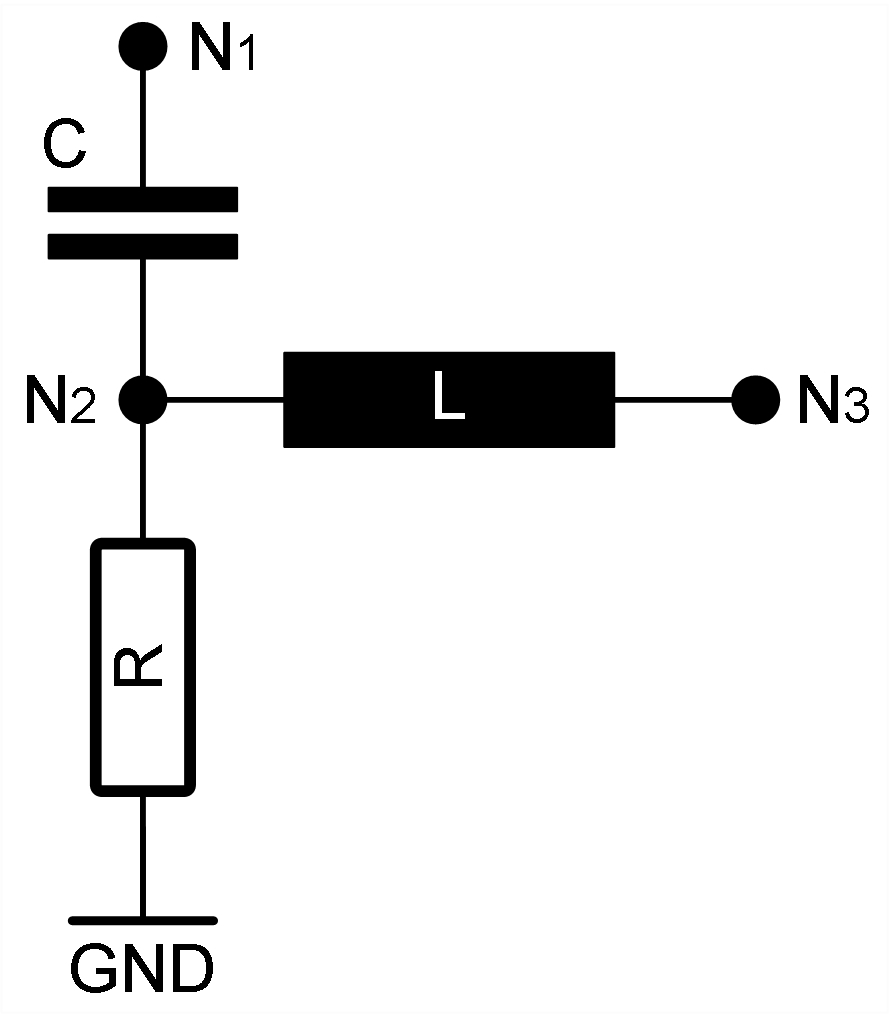
\includegraphics[width=3cm]{LESCreation_fragmentOfPassiveDevices}
  \caption{Fragment of circuit, handling of passive devices}
  \label{figLESCreation_fragmentOfPassiveDevices}
\end{figure}

As usual, the equation system is represented by a matrix. This means only
the coeffcients of the equations are actually represented, the product
with the unknowns $U_{n_j}$ and $U_{n_i}$ is implicit. Which means that
``take a term'' just means to put the symbol $s$ twice in the row of the
matrix, which represents the current balance of node $n_i$: in column $j$
(assuming that this column represents unknown $U_{n_j}$) and as $-s$ in
column $i$ (assuming that this column represents unknown $U_{n_i}$).

The same is repeated for all independent nodes in the circuit. The same
symbol $s$ will appear again, when the process visits node $n_j$. This
time the perspective is inverse and symbol $s$ will appear with inverse
signs in the row that represents the current balance of node $n_j$.

If one of the two nodes the device is connected to should be the ground
node than there is no current balance for this node and one of the two
rows of the matrix containing symbol $s$ will disappear. Same for the
columns, as the ground node's voltage potential doesn't belong to the set
of unknowns. We end up with a single appearance of symbol $s$ in the
matrix.

Figure \ref{figLESCreation_fragmentOfPassiveDevices} shows a fragment of
a circuit. If we assign node $n_i, i=1 \ldots 3$ to row and column $i$ of
our matrix then this fragment would lead to the following matrix:

\begin{displaymath}
\label{eqLESCreation_fragmentOfPassiveDevices}
\left(
\begin{array}{cccc}
-C      & C      &  0     & \ldots \\
 C      & -C-L-R &  L     & \ldots \\
 0      &    L   & -L     & \ldots \\
 \vdots & \vdots & \vdots & \ddots \\
\end{array}
\right)
\end{displaymath}


\subsection{Symbols, knowns and unknowns}

\begin{table}[bt]
\begin{center}
\begin{tabular}{|l|c|p{2cm}|}

\hline

% The column headers:
Kind of device & Substitute of symbol & Meaning \\
\hline
% The next hline makes the column titles a separate rectangular box,
% comment it out to get just a line as separator.
%\hline

\hline

% Table entries start here.
R & \raisebox{0pt}[10pt][5pt]{$\frac{1}{R}$}  & Resistor    \\
Y & $Y$                                       & Conductance \\
L & \raisebox{0pt}[10pt][5pt]{$\frac{1}{Ls}$} & Impedance   \\
C & $Cs$                                      & Capacitor   \\

 \hline
\end{tabular}
\caption{Substitution of symbols in the final result}
\label{tabSubstOfSymbols}
\end{center}
\end{table}

The passive devices don't introduce knowns or additional unknowns to the
equation system.

The name of a device is used as symbol in the internal computation and as
variable in the final result representation. Although it is the same
symbol it has different meanings in either case: In the internal
computation it designates the complex conductance, whereas it has the
common, physical meaning in the final result. For example, $C$ would
actually mean the frequency dependent complex conductivity $Cs$ during the
internal computation but designate the constant, real capacitance in Farad
of a capacitor in the final result.

In the final result representation, the symbols of the internal
computation are substituted by the physical expressions in the complex
frequency variable $s$. This is done according to table
\ref{tabSubstOfSymbols}.

The values for the $R$, $Y$, $L$ and $C$ in the final result, which are
used as default in numeric post-processing with Octave can be found in
table \ref{tabDeviceStdValues} on page \pageref{tabDeviceStdValues}.


\section{Constant voltage source}
\label{secModellingDevs_ConstVoltSrc}

The constant voltage source is a constraint on the LES. The source is
connected to two nodes. These node's voltage potentials, which are both
unknowns to the system are associated by the constraint that they differ
by a constant, given, known voltage.

The constraint is expressed as a simple additional equation, which says
$U_{n_i} - U_{n_j} - U_{ij} = 0$, where $U_{ij}$ is the constant voltage
of the source connected to nodes $n_i$ and $n_j$.

The constant voltage source introduces a further known and thus a further
column to the LES. The additional equation means a further row, too. The
equation is just a triple of signed ones at the according columns. (If the
source is connected to a ground node then only two ones remain.)

The additional equation comes along with an additional unknown. When
setting up the current balance of the connected nodes we have to consider
the additional circuit branch, the current flowing through the source.
This current is unknown. It is defined to be the current flowing out of
the source's plus pole; it's influent and thus positive at the node
connected to the plus pole and affluent or negative at the minus pole's
connetced node. We get a second additional column, which has a pair of
$\pm 1$ as only non null coefficients (or a single signed one if one of
the nodes would be the ground node).

As an example, the source $U_0$ would be connected with its plus and minus
pole between the nodes $N_1$ and $N_3$, respectively, of the circuit
fragment in figure \ref{figLESCreation_fragmentOfPassiveDevices}. The new
unknown current \ident{I\_U0} is put to the right of the unknowns so far
and the new known to the right of the knowns so far. The LES would be
extended to:

\begin{displaymath}
\left(
\begin{array}{ccccccc}
-C      & C      &  0     & \ldots & 1      & \ldots & 0       \\
 C      & -C-L-R &  L     & \ldots & 0      & \ldots &         \\
 0      &    L   & -L     & \ldots & -1     &        & \vdots  \\
 \vdots & \vdots & \vdots &        &        &        & 0       \\
 1      &    0   & -1     & 0      & \ldots & 0      & -1      \\
\end{array}
\right)
\end{displaymath}

Only the constant sources, either voltage or current, introduce the knowns
into the LES. At least one known, hence constant source, is required
otherwise \linnet{} refuses to compute the circuit. The system would
remain unstimulated and all voltages and currents would anyway be null.

If more than one constant source is used then the system changes to a MIMO
system and the result function for an unknown has several terms to
describe the dependency of the unknown on each of the knowns (given a full
results is requested).


\subsection{Symbols, knowns and unknowns}

The source is represented in the LES only as a number of coefficients $\pm
1$ and its name does not appear as a symbol in the internal computation.
It is a known and only apparent in the final result representation. Here,
it has the meaning of the Laplace transform of the given source voltage in
Volt.

The name of the additional unknown, the current through the source is
derived from the device name by adding the prefix \ident{I\_} to the left
of the user-defined device name. The name of the additional unknown does
not appear as a symbol in the internal computation. It can be referenced
in a result specification in order to get an according transfer function
or full result.



\section{Constant current source}

A constant current source is modeled as a known current, which is
influent (i.e. positive) at the node connected to the source's plus pole
and affluent (i.e. negative) at its minus pole's connected node. This
leads to a new column for the additional known, which has just a pair of
$\pm 1$ coefficients at the rows related to the connected nodes (and hence
only a single signed one if one of these nodes is the ground node). All
other coefficients in this column remain null.

As an example, the current source $I_0$ would be connected with its plus
and minus pole between the nodes $N_1$ and $N_3$, respectively, of the
circuit fragment in figure \ref{figLESCreation_fragmentOfPassiveDevices}.
The new known is put to the right of the knowns so far. The LES would be
extended to:

\begin{displaymath}
\left(
\begin{array}{ccccc}
-C      & C      &  0     & \ldots & 1  \\
 C      & -C-L-R &  L     & \ldots & 0  \\
 0      &    L   & -L     & \ldots & -1 \\
 \vdots & \vdots & \vdots &        &    \\
\end{array}
\right)
\end{displaymath}

At least one constant current or voltage source is required otherwise
\linnet{} refuses to compute the circuit; see section
\ref{secModellingDevs_ConstVoltSrc} for more.


\subsection{Symbols, knowns and unknowns}

The source is represented in the LES only as a pair of coefficients $\pm
1$ and its name does not appear as a symbol in the internal computation.
It is a known and only apparent in the final result representation. Here,
it has the meaning of the Laplace transform of the given source current in
Ampere.

The constant current source doesn't add any unknowns to the LES.


\section{The operational amplifier}

% Sample circuit: Op-amp LP 2 times with two different ground nodes
{
% This define is related to the specifics of the array package; see
% http://texwelt.de/wissen/fragen/3401/zentrieren-text-in-tabelle (as of
% July 25 2014) for more
\newcolumntype{M}[1]{>{\centering\arraybackslash}m{#1}}

\begin{figure}[tb]
\begin{center}
\begin{tabular}{M{6cm}M{5.89cm}}
\verbatiminput{OpampLPWithDifferingGnds.cnl}
&
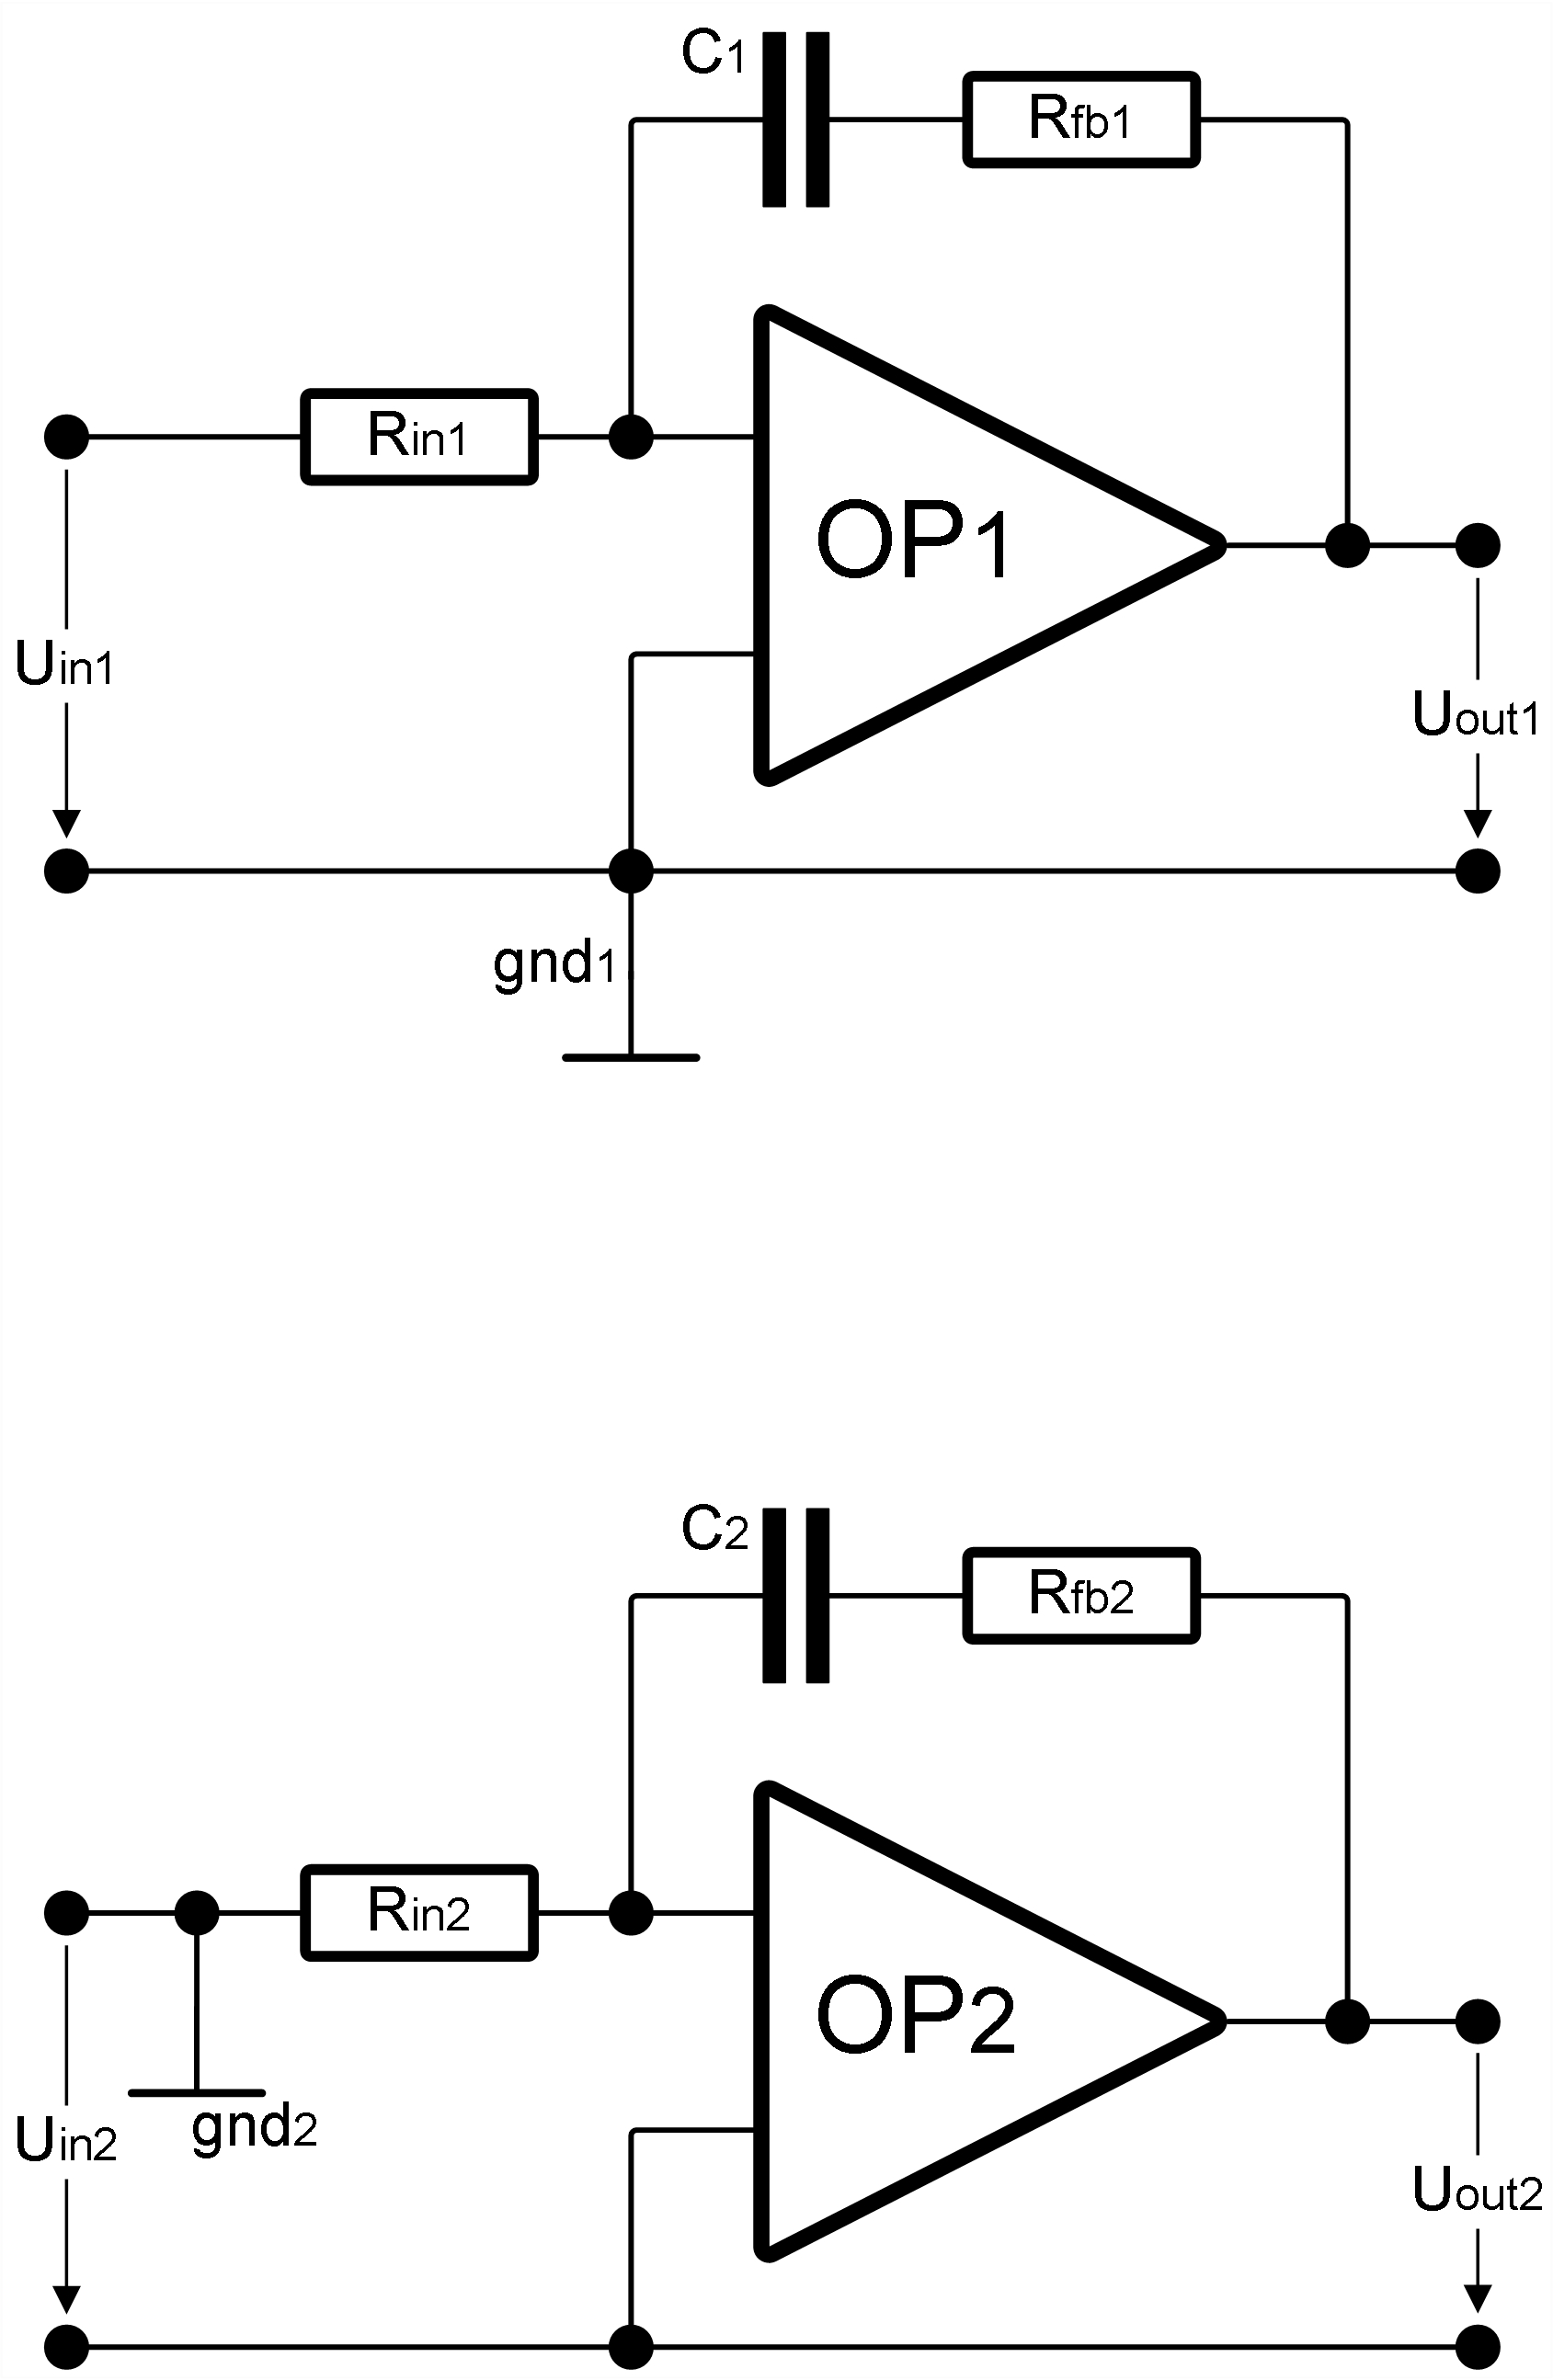
\includegraphics[width=5.89cm]{OpampLPWithDifferingGnds}

\end{tabular}
\caption{Low-pass filter with op-amp and two choices of ground node}
\label{figOpampLPWithDifferingGnds}
\end{center}
\end{figure}
} % Sample circuit: Op-amp LP 2 times with two different ground nodes


Linear operational amplifier circuits are based on the principle, that the
voltage between the two inputs is highly amplified but fed back to one of
the inputs such that the input voltage is compensated till close to null.
The remaining input voltage is in the magnitude of a few micro Volts only
and the output voltage in the magnitude of a few volts. The high dynamic
capabilities of the implementation of the op-amp ensure that this balance
is kept at any time.

The output voltage of the op-amp leads to an output current. This current
is controlled by a push-pull output stage, which lets the output current
flow either from the positive supply voltage or into the negative supply
voltage. (These supply voltages therefore limit the actual output voltage
range.)

The real op-amp is modeled by \linnet{} in an idealized way. The
amplification is made infinite and the feedback by the outer circuitry
thus leads to a voltage of exactely null between the inputs. The dynamic
capabilities become infinitely fast; there's no reaction time, the
equations hold at any time.

Controlling the output voltage by a push-pull output stage is a highly non
linear behavior of the true implementation of an op-amp and can't be
modeled as such by \linnet{}. Instead, \linnet{} approaches this behavior
by a controlled voltage source, which is connected between ground and the
op-amp's output. The voltage is controlled such that the input voltage
becomes null.

Modelling an op-amp like this has several important implications. Most
striking, this model doesn't require any distinction of the two inputs of
the op-amp. The output condition simply is that the input voltage be null;
only the real implementation of the circuitry requires careful selection
of the right input so that the feedback leads to a voltage compensation
rather than to a boost. Contrariwise, any kind of circuit, which founds on
a voltage boost by toggling the inputs (like threshold detector, Schmitt
trigger, etc.) can't simply be modeled with \linnet{}.

Most obvious, there is no output voltage limitation. The output voltage
will raise or drop to any voltage until the condition for the input
voltage is met.

More in general, there is no modelling of the voltage supply at all. Using
an op-amp in \linnet{} only enables to compute the small-signal behavior
of the true circuit; the DC behavior with all supply voltages and currents
and the related power distribution can't be figured out. Furthermore, the
decision to model the output by a voltage source, whose other end is
connected to ground means that the full picture of the solution depends on
the choice of the ground node. An example is given. A low-pass filter is
implemented twice in a single netlist, where the only difference (besides
indexing of the object names) is the different choice of the ground
node. Please refer to figure \ref{figOpampLPWithDifferingGnds}.

\linnet{} computes the same transfer function from input to output voltage
for both variants of the filter. Please compare $U_{out_1}$ with
$U_{out_2}$:

\begin{verbatim}
RESULT - User-defined result G1 (Bode plot):
The dependency of Uout1 on Uin1:
  Uout1(s) = N_Uout1_Uin1(s)/D_Uout1_Uin1(s) * Uin1(s), with
    N_Uout1_Uin1(s) = -Rfb1*C1 * s
                      -1
    D_Uout1_Uin1(s) = Rin1*C1 * s
RESULT - User-defined result Z1 (Bode plot):
The dependency of Uin1 on I_Uin1:
  Uin1(s) = N_Uin1_I_Uin1(s)/D_Uin1_I_Uin1(s) * I_Uin1(s), with
    N_Uin1_I_Uin1(s) = Rin1
    D_Uin1_I_Uin1(s) = 1
RESULT - User-defined result G2 (Bode plot):
The dependency of Uout2 on Uin2:
  Uout2(s) = N_Uout2_Uin2(s)/D_Uout2_Uin2(s) * Uin2(s), with
    N_Uout2_Uin2(s) = -Rfb2*C2 * s
                      -1
    D_Uout2_Uin2(s) = Rin2*C2 * s
RESULT - User-defined result Z2 (Bode plot):
The dependency of Uin2 on I_Uin2:
  Uin2(s) = N_Uin2_I_Uin2(s)/D_Uin2_I_Uin2(s) * I_Uin2(s), with
    N_Uin2_I_Uin2(s) = 1
    D_Uin2_I_Uin2(s) = 0
\end{verbatim}

\begin{figure}[tb]
\begin{center}
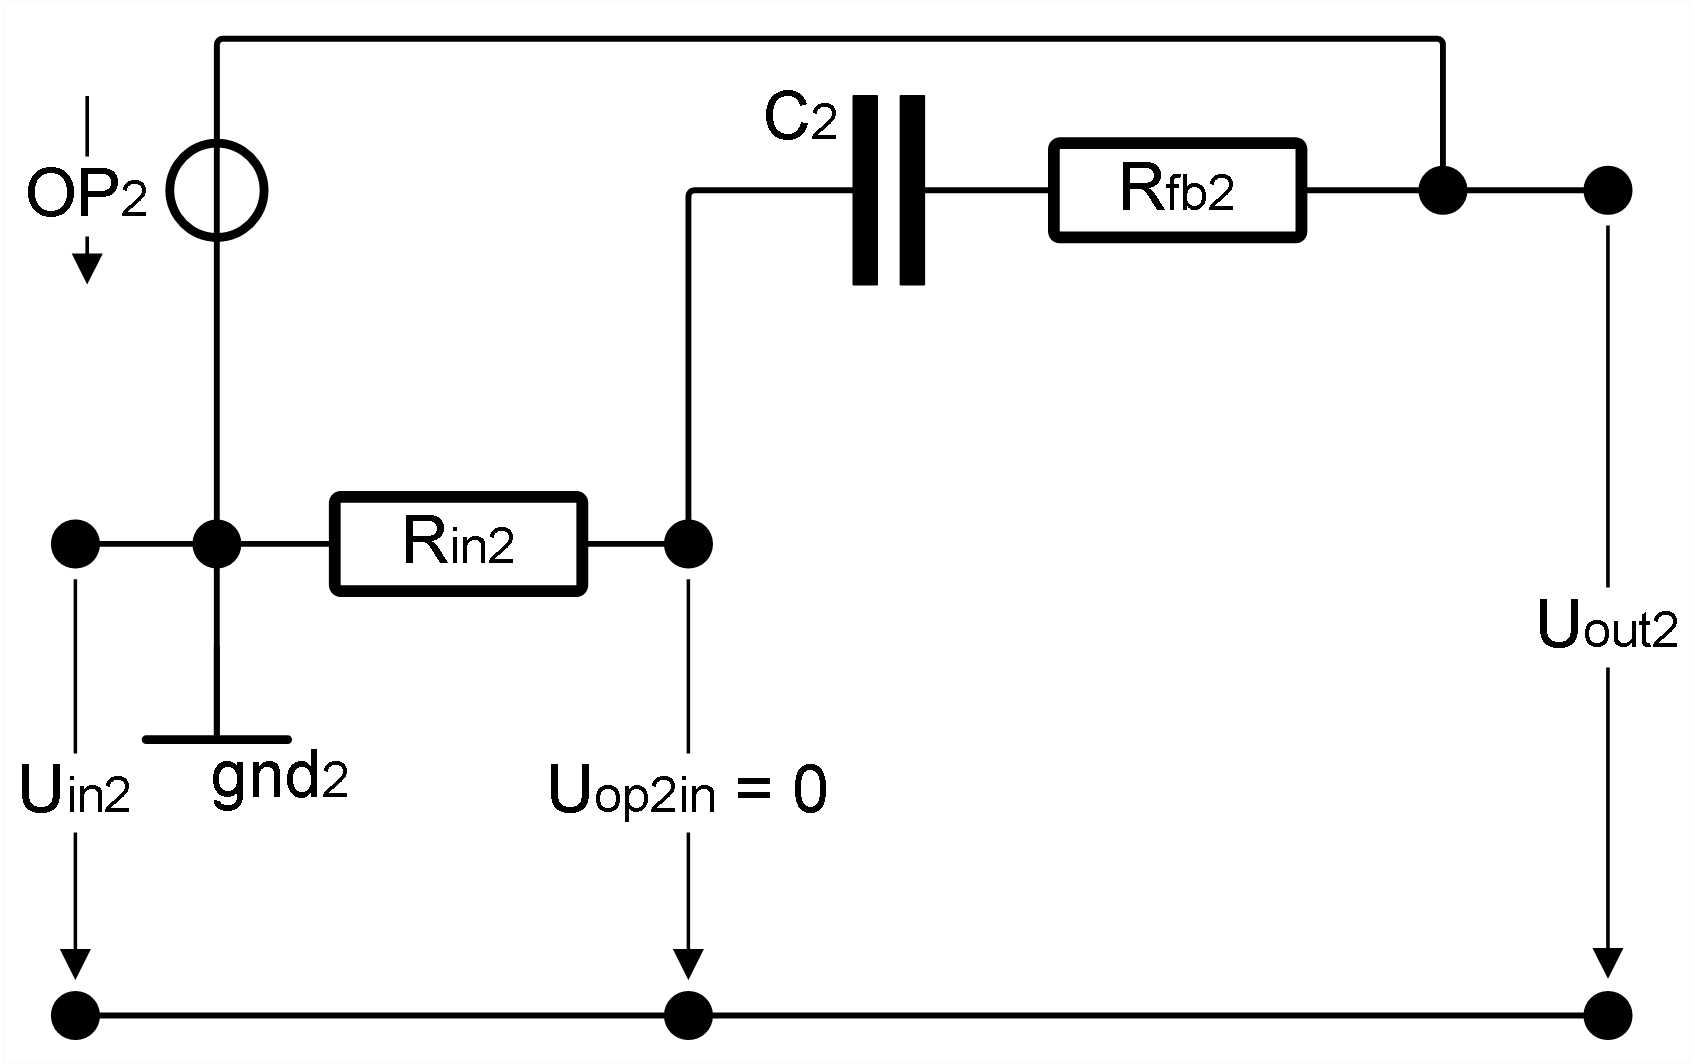
\includegraphics[width=5.96cm]{OpampLPWithDifferingGnds_equivalent}
\caption{Internal, computed model of low-pass filter 2}
\label{figOpampLPWithDifferingGnds_equivalent}
\end{center}
\end{figure}

However, the input impedance (i.e. the transfer function $Z$ from
$I\left(U_{in}\right)$ to $U_{in}$) differs significantly. Variant $1$ of
the filter yields $R_{in}$, which is what we expect but variant $2$ has an
input impedance of infinite (represented by $\frac{1}{0}$ in the result
log). The infinite input impedance is explained by schematic
\ref{figOpampLPWithDifferingGnds_equivalent} that shows how \linnet{}
models the op-amp in this case. The input connectors are open ended and no
current will ever flow into the circuit; this is the meaning of an
infinite input impedance.

It gets even more confusing if we define the node between resistor and
capacitor in the feedback line to be the ground node, please refer to
figure \ref{figOpampLPWithDifferingGnds_variant3}. The controlled voltage
source in \linnet{}'s internal model of the op-amp now doesn't have any
impact on the op-amp's input voltage; the current it can drive only flows
through the resistor in the feedback line. The equation that the op-amp's
input voltage needs to be null can't be fulfilled, the system determinant
is null and the computation fails with error message.

Last but not least the chosen modelling of the op-amp implies that the
output of the op-amp must not be connected to a ground node or to the
output of another op-amp; the controlled voltage source would be
short-circuited in the first case and the system would be underdetermined
in the latter.

An op-amp in the netlist adds a new unknown to the linear equation
system. It is the current flowing from the ground node through the device
and out of its output. The name of this unknown is derived from the name
of the op-amp, the prefix \ident{I\_} is added. 

The new unknown current means a new column in the LES. It contains null
coefficients anywhere but in the row that holds the current balance
of the op-amp's output node. Here, the unknown current is influent and a
one appears as coefficient.

The additional unknown comes along with the new equation $U_{in_1} -
U_{in_2} = 0$. This equation means a row, which has just a pair of $\pm 1$
coefficients at the columns, which are related to the two input node's
voltage potentials (and hence only a single signed one if one of these
nodes is the ground node).

As an example, an op-amp \ident{OP} is connected with its two inputs and
its output to the nodes $N_2$, \ident{GND} and $N_1$, respectively, of the
circuit fragment in figure \ref{figLESCreation_fragmentOfPassiveDevices}.
The new unknown current \ident{I\_OP} is put to the right of the unknowns
so far. The LES would be extended to:

\begin{displaymath}
\left(
\begin{array}{cccccc}
-C      & C      &  0     & \ldots & 1      & \ldots \\
 C      & -C-L-R &  L     & \ldots & 0      & \ldots \\
 0      &    L   & -L     & \ldots & 0      & \ldots \\
 \vdots & \vdots & \vdots &        & \vdots & \ddots \\
 0      & 1      & 0      & \ldots & 0      & 0      \\
\end{array}
\right)
\end{displaymath}


\subsection{Symbols, knowns and unknowns}

The op-amp is ideal and doesn't have a device constant or value. It neither
adds a known to the LES nor a symbol to the computation.

The output current current of the op-amp is a new unknown of the linear
equation system. The name of this unknown is derived from the name of the
op-amp, the prefix \ident{I\_} is added. It can be referenced from a
result definition.


% Same op-amp LP, here with third choice of gnd node
{
% This define is related to the specifics of the array package; see
% http://texwelt.de/wissen/fragen/3401/zentrieren-text-in-tabelle (as of
% July 25 2014) for more
\newcolumntype{M}[1]{>{\centering\arraybackslash}m{#1}}

\begin{figure}[t]
\begin{center}
\begin{tabular}{M{6.5cm}M{5.96cm}}
\verbatiminput{OpampLPWithDifferingGnds_variant3.cnl}
&
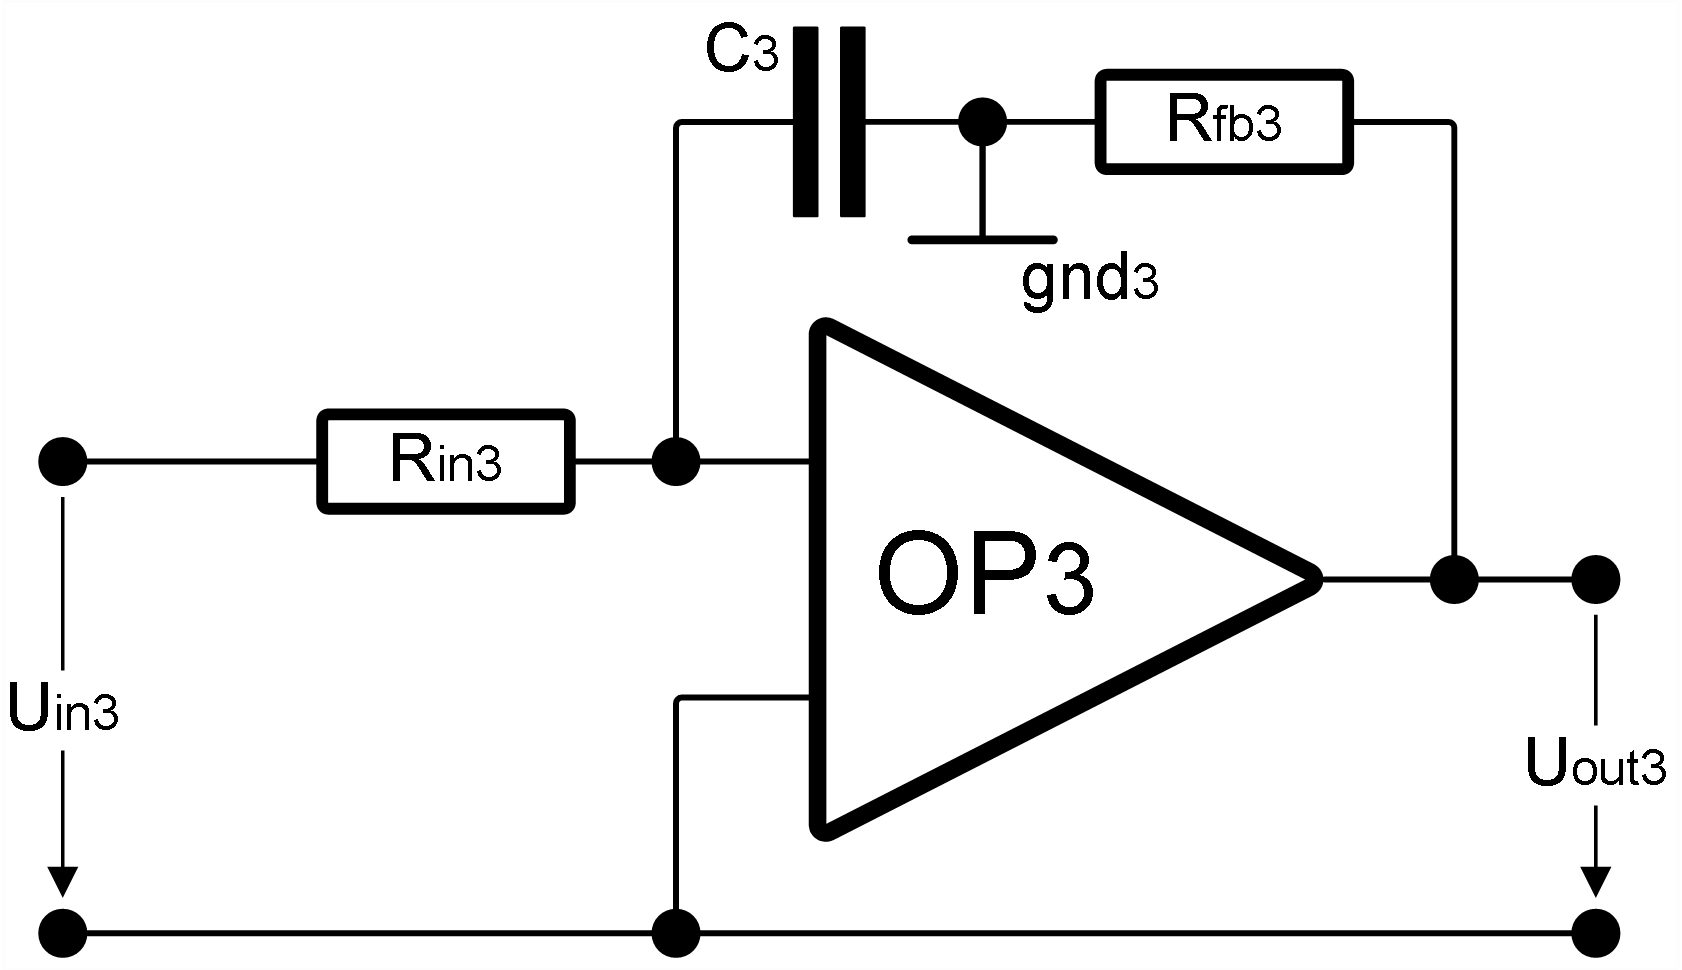
\includegraphics[width=5.96cm]{OpampLPWithDifferingGnds_variant3}

\end{tabular}
\caption{Same low-pass filter with invalid third choice of ground node}
\label{figOpampLPWithDifferingGnds_variant3}
\end{center}
\end{figure}
} % Same op-amp LP, here with third choice of gnd node


\section{Voltage controlled voltage source}

The voltage controlled voltage source is modeled by an additional
equation. The source is connected to two nodes. These node's voltage
potentials, which are both unknowns to the system are associated by the
constraint that they differ by a constant multiple $k$ of a voltage, which
is unknown but which can be expressed as difference of two nodes. The
multiple $k$ is the device constant and is a new symbol in the
computation.

The additional equation is $U_{n_i} - U_{n_j} - kU_{n_u} + kU_{n_v} = 0$;
the voltage source is connected to nodes $n_i$ and $n_j$, $k$ is its
dimensionless device constant and the control voltage is the voltage
potential difference between the nodes $n_u$ and $n_v$.
 
The additional equation means a further row to the LES, which has all null
coefficients but a pair of $\pm 1$ and a pair of $\pm k$. (Both pairs can
reduce to a single signed one or $k$ if one of the references nodes is a
ground node. If both nodes of the control voltage are the ground node then
the $\pm k$ will even disappear entirely.)

The additional equation comes along with an additional unknown. When
setting up the current balance of the nodes the source is connected to we
have to consider the additional circuit branch, the current flowing
through the source. This current is unknown. It is defined to be the
current flowing out of the source's plus pole, which is the first
connected node. This current is influent and thus positive at the node
connected to the plus pole and affluent or negative at the minus pole's
connected node. We get an additional column in the LES, which has a pair
of $\pm 1$ as only non null coefficients (or a single signed one if one of
the connected nodes would be the ground node).


\subsection{Symbols, knowns and unknowns}

The voltage controlled voltage source doesn't introduce knowns to the
equation system.

The name of the device appears as a symbol in the internal computation and
in the final result. It has the meaning of the source's dimensionless
voltage amplification $k$. The value for $k$ used as default in numeric
post-processing with Octave can be found in table \ref{tabDeviceStdValues}
on page \pageref{tabDeviceStdValues}.

The name of the additional unknown, the current through the source is
derived from the device name by adding the prefix \ident{I\_} to the left
of the user-defined device name. This name does not appear as a symbol in
the internal computation. It can be referenced in a result specification
in order to get an according transfer function or full result.


\section{Current controlled voltage source}

The current controlled voltage source is modeled by an additional
equation. The source is connected to two nodes. These node's voltage
potentials, which are both unknowns to the system are associated by the
constraint that they differ by a constant multiple $k$ of a current, which
is an unknown of the LES. (It is the unknown current through a current
probe; please refer to section \ref{secModellingDevs_currentProbe} for
details.) The multiple $k$ is the device constant and it is a new symbol
in the computation.

The additional equation is $U_{n_i} - U_{n_j} - k I_c = 0$;
the voltage source is connected to nodes $n_i$ and $n_j$, $k$ is its
device constant and $I_c$ is the control current, an unknown of the LES.

The additional equation means a further row to the LES, which has all null
coefficients but a pair of $\pm 1$ (or a single signed one if one of the
connected nodes would be the ground node) and a single signed $k$.

The additional equation comes along with an additional unknown. When
setting up the current balance of the nodes the source is connected to we
have to consider the additional circuit branch, the current flowing
through the source. This current is unknown. It is defined to be the
current flowing out of the source's plus pole, which is the first
connected node. This current is influent and thus positive at the node
connected to the plus pole and affluent or negative at the minus pole's
connected node. We get an additional column in the LES, which has a pair
of $\pm 1$ as only non null coefficients (or a single signed one if one of
the connected nodes would be the ground node).


\subsection{Symbols, knowns and unknowns}

The current controlled voltage source doesn't introduce knowns to the
equation system.

The name of the device appears as a symbol in the internal computation and
in the final result. It has the meaning of the source's current to voltage
amplification $k$. The value for $k$ used as default in numeric
post-processing with Octave can be found in table \ref{tabDeviceStdValues}
on page \pageref{tabDeviceStdValues}.

The name of the additional unknown, the current through the source is
derived from the device name by adding the prefix \ident{I\_} to the left
of the user-defined device name. This name does not appear as a symbol in
the internal computation. It can be referenced in a result specification
in order to get an according transfer function or full result.


\section{Voltage controlled current source}

The voltage controlled current source is modeled similar to a passive
device. By definition, the current flowing through the voltage controlled
current source is described by $I = k(U_{n_u} - U_{n_v})$, where $k$ is
the device constant, the amplification from voltage to current, and the
control voltage is the voltage potential difference between the referenced
nodes $n_u$ and $n_v$.

This current is considered when setting up the current balance of the two
nodes the source is connected to. It is defined to be the current flowing
out of the second node in the netlist and it is influent and thus positive
at this node. Vice versa, it is flowing back into the source at the first
node in the netlist or affluent or negative at this node. In each of the
two affected rows of the LES we get a pair of $\pm k$ as further addends
of the coefficients of the unknown voltage potentials of the two
referenced control nodes. (If one of the connected nodes is the ground
node or if one of the nodes that define the control voltage is the ground
node then two of the $\pm k$ disappear; if both holds then only a single
signed $k$ remains.) The appearance pattern of symbol $k$ in the LES is
nearly the same as for the passive devices; the only difference is the
possible appearance as a single pair $\pm k$. Neither an additional known,
unknown nor equation is required.


\subsection{Symbols, knowns and unknowns}

The voltage controlled current source neither introduces knowns nor
unknowns to the equation system. In particular, there's no unknown, which
describes the current through the source. If this current is needed in a
user-specified result then a current probe needs to be placed in series
with the source.

The name of the device appears as a symbol in the internal computation and in
the final result. It has the meaning of the source's voltage to current
amplification $k$. The value for $k$ used as default in numeric
post-processing with Octave can be found in table \ref{tabDeviceStdValues}
on page \pageref{tabDeviceStdValues}.


\section{Current controlled current source}

By definition, the current flowing through the current controlled current
source is described by $I = kI_c$, where $k$ is the device constant, the
dimensionless amplification from control to output current, and $I_c$ is
the control current. $I_c$ is the the current through a current probe
device and such a current always is an unknown of the LES. (Please refer
to section \ref{secModellingDevs_currentProbe} for details.)

The current $I$ is considered when setting up the current balance of the
two nodes the source is connected to. It is defined to be the current
flowing out of the second node in the netlist and it is influent and thus
positive at this node. Vice versa, it is flowing back into the source at
the first node in the netlist or affluent or negative at this node. A pair
of $\pm k$ appears in the column of the LES that belongs to the unknown
control current $I_c$ (or a single signed $k$ if one of the connected
nodes is the ground node). Besides null coefficients this column can also
contain the same pattern from other instances of such sources, if they are
controlled by the same unknown current, and it will contain a pair of $\pm
1$ from the referenced current probe itself. If the devices share their
connected nodes then these ones and symbols share the same row, they
become addends of the coefficient of the LES.

Neither an additional known, unknown nor equation is required.


\subsection{Symbols, knowns and unknowns}

The current controlled current source neither introduces knowns nor
unknowns to the equation system. In particular, there's no unknown, which
describes the current through the source. If this current is needed in a
user-specified result then a current probe needs to be placed in series
with the source.

The name of the device appears as a symbol in the internal computation and
in the final result. It has the meaning of the source's dimensionless
current to current amplification $k$. The value for $k$ used as default in
numeric post-processing with Octave can be found in table
\ref{tabDeviceStdValues} on page \pageref{tabDeviceStdValues}.


\section{The current probe}
\label{secModellingDevs_currentProbe}

The current probe is an ideal wire, which connects two nodes. The voltage
potentials of these two nodes become identical. As a kind of side-effect
the current through this wire becomes a new unknown of the LES and can be
queried in result specifications.

Actually, the current probe is a constant voltage source with voltage
null. Please refer to section \ref{secModellingDevs_ConstVoltSrc} to see
how such a source is modeled. The current probe is different in two
aspects: The way, the name of the new unknown is derived from the device
name is different and no additional known (the constant source voltage) is
introduced to the LES since the voltage is null by definition. All
according terms of the result would have to be taken times null anyway.

The polarity of the unknown current through the current probe is defined
as for the current sources: The unknown current is the one, which flows
out of the second connected node into the network and from the network
node, which is mentioned first in the netlist back into the probe. This
sounds counter-intuitive but isn't: This way, the first and second netlist
node mean the start and end of the arrow in the symbol of the current
probe in this order (see table \ref{tabSupportedDevices} on page
\pageref{tabSupportedDevices}).


\subsection{Symbols, knowns and unknowns}

The current probe doesn't introduce a known to the equation system.

Neither in the internal computation and nor in the final result will the
name of the device appear as a symbol.

The name of the additional unknown, the measured current, is basically
derived from the device name by adding the prefix \ident{I\_} to the left
of the user-defined device name -- as usual for the sources. However, if
the device name already starts with the character sequence \ident{I\_} then
this name extension doesn't take place and the name of the unknown current
is identical with the name of the device. This has been decided for
convenience: It's natural to name a current probe like the measured
current but this must not lead to names like \ident{I\_I\_measured}.
Sticking to the common naming pattern would mean to force the user to name
the current probe device only \ident{measured} in this example, which was
a degradation of the readability of the netlist.

The name of the measured current does not appear as a symbol in the
internal computation. It can be referenced in a result specification in
order to get an according transfer function or full result.

\chapter{Building \linnet{}}
\label{secBuildingLinNet}

\linnet{} is distributed as source code together with makefiles to compile
and link the code. The distribution contains ready-to-use binaries for
Windows, for both the win32 and win64 ABI and as debug or production
compilation\footnote{Windows 7 has been used.}. In all other environments
a build of the sources needs to be done prior to the use of \linnet{}.

To start the build you need to \code{cd} in a shell window to the root
directory of the \linnet{} distribution, where the file \file{GNUmakefile}
is located. Here, you issue the command:
\begin{verbatim}
make build
\end{verbatim}
The makefile has some more useful targets and options than just
\ident{build}. Tpye \code{make help} to find out.


\section{Portability of makefiles}

The makefile -- actually it is a set of nested makefiles -- is compatible
with the GNU make processor of at least revision 3.81; 3.80 is not
sufficient. Different derivates of make always tended to be quite
incompatible to one another and other derivates of make will hence need
heavy modifications of the makefiles.

The makefiles directly support the build of the software for Windows with
GCC in the MinGW 32 and 64 Bit ports. The compilation and the compiled
software have been tested with GCC 4.5.2 (32 Bit) and 4.8.1 (64 Bit) and
under Windows 7 only. Other revisions may cause problems: Even between
these two severe incompatibilities have been found, which had to be
tackled by conditional code (see below).

The makefile needs to know, where GCC is installed. For Windows systems
the environment variable \ident{MINGW\_\-HOME} has been introduced. It may
be used to specify the root folder of a MinGW installation. If it is set,
either persistently or on the command line of the make processor -- e.g.
to be able to switch between 32 Bit and 64 Bit builds -- then the
directory \file{\$\{MINGW\_\-HOME\}/bin} supersedes the normal system
search path. If the variable is not set then all executables will be
located via the system search path as specified in environment variable
PATH. This would be the natural choice for a Linux system. Please refer to
file \file{locateTools.mk} for details.\footnote{Although designed for
Windows, where typically several different competing ports of GCC can
reside, the environment variable can be used for Linux and Mac OS, too.
Don't bother with the name but let the variable point to the parent folder
of GCC's bin folder.}

The makefiles are designed to support the compilation under Linux and Mac
OS also. GNU make's \code{if}/\code{else}/\code{endif} statements have
been applied to do so. As of today, this has been tested with a single Linux
distribution only (Fedora 18) and might not work out of the box for other
environments. Particularly, you should have a look at the tool
localization in \file{locateTools.mk} and the compiler and linker command
line options in \file{compileAndLink.mk}.


\subsection{Resource compiler}

Under Windows the application icons are added to the executable binary
file. This has no functional aspect; the image data is not accessed from
the functional code. It's just a gimmick that allows to create illustrated
associations between \linnet{} in- and output files and the executable in
the file system browser.

In the makefile the according build rules are placed in
\code{if}/\code{endif} clauses; they should have no effect under either
Linux or Mac OS. Similar mechanisms will probably exist for these operating
systems as well. You may consider to extend the makefiles by adding
appropriate \code{else} paths; an OS indicating variable already exists.


\section{Portability of source code}

The source code itself is system independent; only the abstract functions
from the GNU C library are used. The sources have been compiled and linked
without errors and warnings with GCC 4.5.2 (32 Bit) and 4.8.1 (64 Bit),
both Windows 7, and GCC 4.7.2 under Linux in the Fedora 18-i686
distribution.

The compilation with a different compiler tool chain (including another
revision or port of GCC) will probably introduce some changes on the
source files. The applied compiler needs to support the standard C99.


\subsection{GNU extensions}

In module \ident{rat\_rationalNumber} a GNU extension is used: Initialized
structs are used as RHS of assignment expressions. This has been done
for convenience only, to achieve at tense and meaningful representation of
the required functionality. It should however be easy and straightforward
to eliminate these (few) constructs. All the rest is according to the
standard C99.


\subsection{Incompatibilities of linked libraries}

Far the most necessary code modifications will result from
incompatibilities of the linked libraries. Most obvious is the use of
GCC's Basic Program/System Interface, the command line evaluation support.
All of the command line evaluation related code will probably require a
complete re-implementation with another compiler tool chain. Please refer
to module \ident{opt\_getOpt} for details.

The two tested ports of GCC have different sets of standard functions. The
MinGW 64 Bit port provides \ident{stricmp} while MinGW 32 Bit doesn't. A
simple implementation of this function has been added to the \linnet{}
sources. Depending on the availability of this function in your
environment you will have to modify the according preprocessor switches to
let it or don't let it compile the substitute. Please refer to file
\file{stricmp.h} for details.

The standard function snprintf was found to be buggy in the used 64 Bit
port of GCC. A work around has been implemented, which is compiled only
for the 64 Bit MinGW ports. You will have to check if your revision of GCC
has the same problems and maybe have to modify the preprocessor code that
controls the conditional compilation of the substitute. Please refer to
file \file{snprintf.h} for details.


\section{Re-entrance of code}

The implementation of \linnet{} is widely but not completely reentrant.
This can become an issue if the code should be integrated into a
concurrent environment; for example a client-server structure is set up or
multi-core support is implemented to speed up the computations. As long as
the code is used as of today in a single-threaded self-contained
application the following considerations are irrelevant.

Although the implementation of module \ident{log\_logger} is made in a reentrant
style, the logging process is not reentrant by principle. All logger
instances write to the same global stream \ident{stdout} and concurrent
use would lead to a mess of text at the console. Furthermore, all modules
of \linnet{} use one and the same global logger instance and they hence
share the same file stream, too; here, we'd expect a similar mess.

For module \ident{pci\_parserCircuit}, the parser of the circuit netlist
files, the decision to use a few global variables (e.g. for error
reporting by side effect) has just been taken for convenience, to keep the
code lean. An application for a fully reentrant implementation was simply
not in the scope of the development. It's however straightforward and only
little effort to make the parser reentrant. One just has to put the few
global variables into a struct, which gets the meaning of a parser
instance, add a constructor/destructor pair and pass the pointer to the
parser instance to all the functions.

The situation differs for the other affected module
\ident{rat\_rationalNumber}, the implementation of an exact arithmetics
for rational numbers. Here, the decision to use global data and to loose
re-entrance has been taken intentionally for performance reasons. A global
variable is used to report an overflow. In addition, a global logger
instance is used to visibly report problems. This logger isn't reentrant,
neither. The client code can check the global variable after completing
the operations. The flag is persistent and can thus be checked after a
bunch of operations as an overall result. To avoid the flag we could
return the overflow indication with every operation but this would lead to
a manifold of computational effort. Or we could introduce rational number
processor instances having each their own individual error handlers. The
overhead of passing the instance pointer to all the functions would
probably be less than in the first suggestion but still significant.

If the software is used in an environment, where re-entrance is a must then
serialized access to the module could also be an option. A client is
queued until the other one has completed its (bunch of) operations and has
checked the global error information.
\chapter{Understanding the Octave Interface}
\label{secOctaveInterface}

\section{Folders, files and functions}

If the switch \code{-o} is put on the command line of \linnet{} then the
computed formulas are exported to Octave in form of a set of generated
scripts (files \file{*.m}). Octave needs to be installed in order to make
any use of these files. A further prerequisite is the availability of
package control, which should normally be installed with
Octave.\footnote{Type \code{pkg list} in the Octave command line to find
out.} Please visit http://www.gnu.org/software/octave/ for information and
download.

One dedicated script is generated for each of the results specified in the
netlist file. The script has the name of the result in the netlist file.
If no result is specified in the netlist file then \linnet{} uses the
implicit result definition \ident{allDependents} and the generated Octave
script has this name, too. All of the result related scripts are bundled
in a common folder, which is also created and which has the name of the
netlist file (except for the removed name extension). Several such folders
will be created if the \linnet{} command line specifies several netlist
files. All of the created folders are placed in a common target directory,
which can either be specified as argument of command line option \code{-o}
or defaults to the current working directory. This directory needs to
exist, \linnet{} won't create it.

The generated, result related Octave scripts implement Octave functions.
The functions in turn have the name of the result in the netlist file.
They are self-contained in the sense that they can be called just like
that if only the current working directory in the Octave session is the
folder containing the script file, i.e. the folder that has the name of
the processed netlist file. If you \code{cd} to the created folder and
type the name of the result then you should get an Octave figure window
with either a step response or a Bode plot -- which one depends on the way
the result was defined. The details of the result definition can be found
at \ref{secResultSpec} on page \pageref{secResultSpec}.

The next step should be to type \code{help} followed by the name of the
result.

The generated result related scripts use some (simple) sub-routines. These
subroutines are implemented as a set of Octave files, which are bundled in
folder \file{private} that is found inside the created netlist related
result folder. The contents of folder \file{private} are invariant. As a
matter of fact, the whole folder is just the copy of a template folder
located somewhere in the installation of \linnet{}. Therefore, getting
this folder in every netlist related result folder is actually not
essential and may even become annoying. (The design decision to do so has
been taken for convenience, to make the result scripts self-contained and
immediately usable.) To avoid these redundant files you can consider to
make a copy of the files in the private folder into any folder holding
Octave script files and to add this other folder to the Octave search
path. From now on you would run \linnet{} with command line option
\code{-i} and folder \file{private} is no longer generated in the created
result folders. The copied files on the Octave search path will be used
instead of those in folder \file{private}.


\section{The two kinds of generated Octave functions}

Depending on how a user-defined result is specified in the netlist file
the generated Octave script will define a function of one out of two
possible kinds. If the netlist command \code{PLOT} is used then the
generated Octave function will show the Bode plot of a transfer function (or
frequency response) of the system or one of its variables. If the netlist
command \code{RES} is used then the generated Octave function will show
the step response of the system or one of its variables.

The plots are presented if the function is called without assignment of
the (optional) return values. The simplest way to do so is to just type
the function name (i.e. result name) on the Octave command line.


\section{Symmetries between the two kinds of generated Octave functions}

Regardless of the fundamentally different plots the two kinds of generated
Octave functions are quite similar.

Both kinds of functions have (nearly) the same signature. The difference
is only their internal behavior, the internal decision to chose an
appropriate kind of plot and this behavior is inhibited if a return value
of the function is consumed by the calling code. If so, both kinds of
functions behave identical: They generate and return the LTI object and
maybe the parameter set and a default vector of either frequency values or
time designations. (This last, optional return value is the only remaining
difference in the behavior of the two kinds of functions.) As the first
two return values are far the most relevant ones, both kinds of functions
can mostly be used in an identical fashion. This means for example, that a
Bode plot result can easily be used to plot a step response and vice
versa:

Be \file{G.m} an Octave script generated from a \code{PLOT} command and
\file{I\_Uin.m} an Octave script generated from a \code{RES} command then
will the direct call of
\begin{itemize}
  \item \code{G} open a figure window with the Bode plot of (transfer
    function) $G$. This is the internal behavior of \code{PLOT} generated
    M functions,
  \item \code{I\_Uin} open a figure window with the step response of
    (current) $I_{U_{in}}$. This is the internal behavior of \code{RES}
    generated M functions.
\end{itemize}
In contrast to this will a the first return value consuming call like
\begin{itemize}
  \item \code{step(G)} open a figure window with the step response of the
    system described by (transfer
    function) $G$,
  \item \code{bode(I\_Uin)} open a figure window with the Bode plot of the
    transfer function from system input $U_{in}$ to current $I_{U_{in}}$.
\end{itemize}
Please note, that this is an example. In general, there are constraints.
As an example, Octave refuses the Bode plot for systems other than SISO.

Using the generated M functions as argument of enclosing Octave
expressions works well but is somewhat slow: Each time the
expression is evaluated another (temporary) LTI object is created by the
function. This causes a noticeable delay. In most situations it will be
more appropriate to create the LTI object once in the workspace and to
continue with the same object. The commands from the last example would
change to:
\begin{verbatim}
  tfG = G; step(tfG)
  tfI_Uin = I_Uin; bode(tfI_Uin)
  ...
  nyquist(tfG)
\end{verbatim}
The last line is just meant to demonstrate how to benefit from the once
and only once created objects.


\section{Varying device values}

A netlist file, which is the source of the Octave scripts that create the
LTI objects, has the option to specify device values. This applies to the
passive devices and the controlled sources. A resistor can get a value,
which is understood as resistance in $\Omega$, a conductance can get a
value in $\frac{1}{\Omega}$, the capacitor is understood in $F$ and the
impedance in $H$. The device values of controlled sources are understood
as the proportionality factor between control voltage/current and controlled
voltage/current. Accordingly, they are dimensionless or understood as
either $\frac{A}{V}$ or $\frac{V}{A}$.

If the netlist specifies a device value then this value is put into the
generated Octave script as default value for all numeric computations. For
\linnet{} itself the value is meaningless, it is not used at all by any
\linnet{} computation.

All devices which no value is specified for in the netlist will get a
hard coded standard value as default value in the generated Octave script.
These standard values depend on the kind of device but do not consider
values, which might have been specified in the netlist for other devices. A
mixture of explicitly specified device values and standard values in one
and the same netlist file is not recommended.

\begin{table}[bt]
\begin{center}
\begin{tabular}{|l|c|c|l|}

\hline

% The column headers:
Device & Symbol & Value & Remark \\
\hline
% The next hline makes the column titles a separate rectangular box,
% comment it out to get just a line as separator.
%\hline

\hline

% Table entries start here.
Resistor                          & R    & 100 $\Omega$     & RLC should yield audio frequencies \\
Conductance                       & Y    & 10 mS            &                                    \\
Capacitor                         & C    & 10 $\mu F$       &                                    \\
Impedance                         & L    & 1 mH             &                                    \\
Voltage controlled voltage source & U(U) & 1                & No particular use case aimed       \\
Current controlled voltage source & U(I) & 1 $\frac{V}{A}$  & No particular use case aimed       \\
Voltage controlled current source & I(U) & 5 $\frac{mA}{V}$ & Use case unipolar transistor       \\
Current controlled current source & I(I) & 250              & Use case bipolar transistor        \\

\hline

\end{tabular}
\caption{Device standard values}
\label{tabDeviceStdValues}
\end{center}
\end{table}

The hard coded standard values are chosen such that if no device values are
specified in the netlist then the time constants of the system will
probably be in the audio frequency range. This holds for the values of
the four passive device kinds.

The standard values for the controlled sources are more difficult to
choose. Such sources can be used to model totally different physical
effects and a prototypic value is hard to find. If there is a typical use
case like the bipolar transistor simulation with a current controlled
current source then this use-case has let to the chosen standard value.
Because of the difficult definition of these standard values it is
recommended not to use controlled sources in numerical evaluations with
Octave without the explicit specification of a realistic device value in
the netlist.

All hard coded standard values of all affected devices are listed in table
\ref{tabDeviceStdValues}.

The values -- either explicitly specified or standard values - are written
into the generated Octave script and used if the scripts are run without
more ado. In the Octave session they can be accessed and changed. This way the
numeric system simulation can be repeated with altered values and the
system behavior can be investigated in dependency of device value changes
in an empiric way. 

The second return value of the generated Octave functions is a
\code{struct}. The members have the names of the devices. Each member holds
the value of the related device. The struct implements the parameter set
the returned LTI object has been created from.

The third return value of the generated Octave functions depends on the
kind of result, Bode plot or full result. It is a vector of frequency
values or time designations, respectively. Frequency values have the unit
$\frac{rad}{s}$ as common for Octave functions. The retrieved vector is a
suitable starting value for system simulations and can be used with the
Octave functions \ident{bode}, \ident{step}, \ident{impulse}, etc. It
depends on the kind of command, whether a frequency or time vector is
required.

Calling the generated function with consumption of at least one return
value inhibits the internal behavior; no figure window is opened, no plot
is made. Just the mentioned data is fetched if the return values are
assigned to workspace variables. These variables can then be altered and
reused for subsequent computations.

The generated functions take a parameter set as only (optional) argument.
In most cases, the parameter set will be the modified return value of a
previous call of the function. Providing this argument makes the functions
behave exactly as before but only using the altered parameters. You can
either let them plot the standard figures (Bode plot or step response) or
let them create a \emph{new} LTI system object based on the altered
parameters. Please note, it is not possible to change the parameters of a
previously created, already in the workspace existing LTI object; instead,
you will always have to replace or overwrite it.

Varying the device constants or parameters of a circuit is now completed
with an example. Be \file{G.m} the generated Octave script:

% The flushleft (table left-aligned) in conjunction with @{} (cell
% contents without leading blanks space) ensures left-aligned appearance
% of the M code.
%   The \hspace* at the end of the longest M code cell enlarges the
% distance of code and explanations.
\begin{flushleft}
\begin{tabular}{@{}ll}
\verb+G+             & \% Plot the transfer or step function as defined in the circuit file \\
\verb+[tf_G p] = G+  & \% Get an LTI object (class tf) and the default set of device constants \\
\verb+p.R1 = 330;+   & \% Modify device constant $R_1$ in parameter set \ident{p} \\
\verb+p.R2 = 2*p.R1+
\hspace*{8mm}        & \% Modify device constant $R_2$ in parameter set \ident{p} \\
\verb+G(p)+          & \% Repeat the initial plot with the altered parameter set \ident{p} \\
\verb+tf_G = G(p)+   & \% Replace the LTI object with a new one using the altered device constants\\
\verb+step(tf_G)+    & \% Plot the step response of the system with modified device constants \\
\verb+bode(tf_G)+    & \% Plot the transfer function with modified device constants \\
\verb+nyquist(tf_G)+ & \% Nyquist plot with modified device constants \\
%\verb++ & \%  \\

\end{tabular}
\end{flushleft}


\section{Caveats of Octave}

Although generally working well, has using Octave for numerical
post-processing some weaknesses. The author has solely used Windows
ports of Octave which might be worse than Linux releases with respect to
functional failures and stability. The following is stated only for the
Windows ports of release 3.4.3 and 3.6.4 running under Windows 7.

Octave 3.6.4 has general problems with the figure windows. The chosen
graphics back-end was ``fltk''.
\begin{itemize}
  \item The opened figure windows are initially black. The actual plots
    appear only after some clicking into the window pane or on the
    buttons to enforce a redraw    
    
  \item If the figure window is enlarged by dragging the corners with the
    mouse than only the frame of the window is resized, the contents stay
    the same. This is particular annoying when MIMO systems produce grids
    of plots; these are initially tiny but can't be enlarged
\end{itemize}

These problems let to the decision to continue with the elder release
3.4.3. Window handling is okay in this release.

With Octave 3.4.3 we get a reproducible crash when running result \code{G}
of netlist file
\file{bandStop.makesOctave3-4-3-win32Crash.cnl}.\footnote{The file is
contained in the source distribution of \linnet{}.} The \linnet{}
generated file \file{G.m} looks however unsuspiciously and resembles
dozens of other generated files which are successfully processed. Octave
3.6.4 and MATLAB process file \file{G.m} successfully and plot the
expected result.

\chapter{Typical Use Cases}

\section{Transfer function and full result}

\subsection{SISO system}

The most common use case of \linnet{} is the computation of the frequency
response of a single in- and output system. This use case demonstrates how
such a basic investigation can be done with \linnet{}.

% Use case SISO: OP filter with two time constants.
{
% This define is related to the specifics of the array package; see
% http://texwelt.de/wissen/fragen/3401/zentrieren-text-in-tabelle (as of
% July 25 2014) for more
\newcolumntype{M}[1]{>{\centering\arraybackslash}m{#1}}

\begin{figure}
\begin{center}
\begin{tabular}{M{6cm}M{5.4cm}}
{\normalsize
\verbatiminput{UseCaseOpFilter.cnl}
}
&
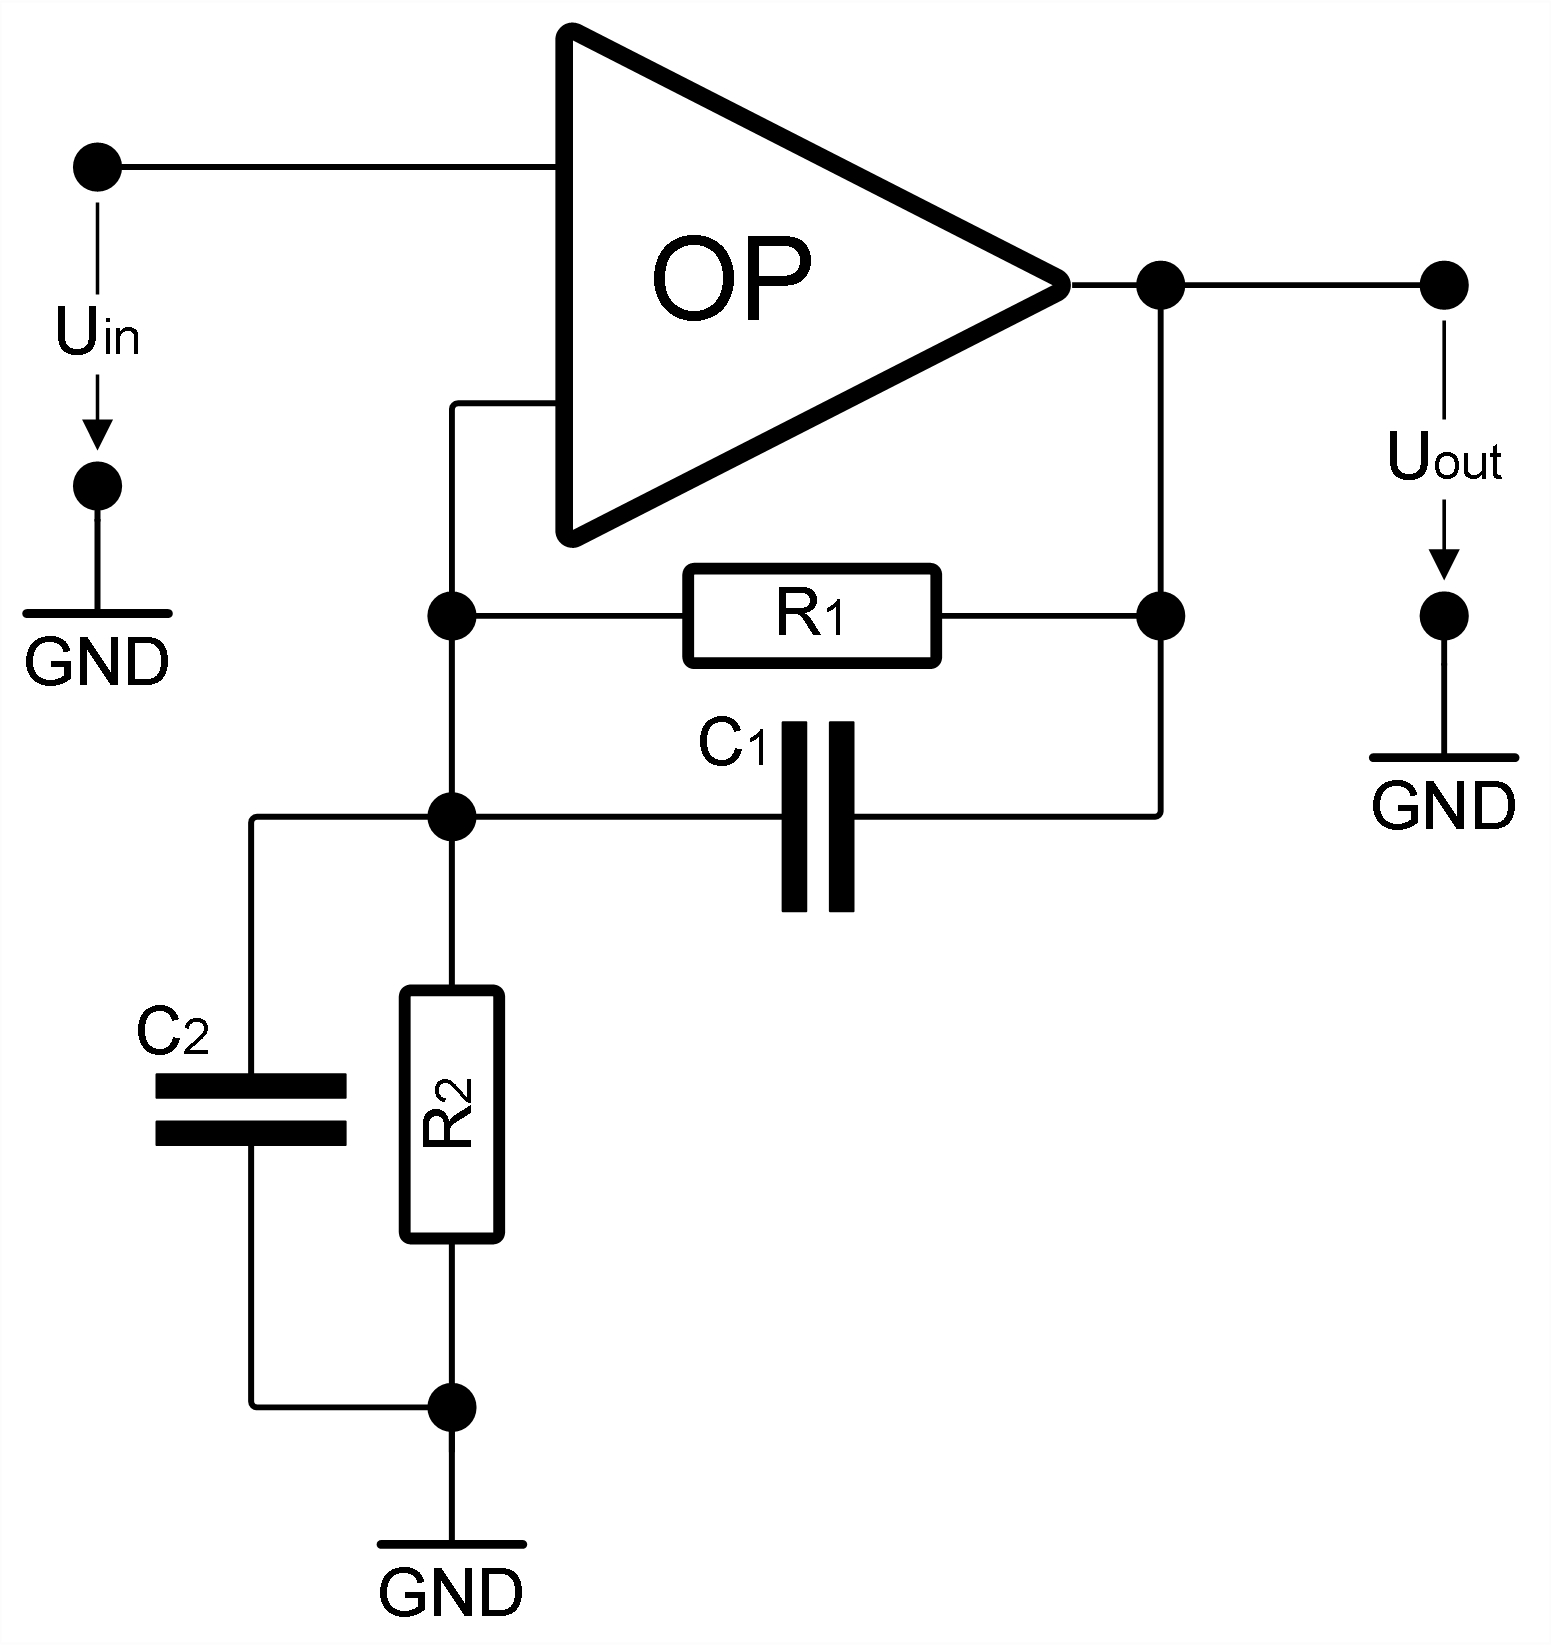
\includegraphics[width=5.4cm]{UseCaseOpFilter}
\\

\end{tabular}
\caption{Op-amp filter with two time constants}
\label{figUseCaseOpFilter}
\end{center}
\end{figure}
} % End of figure use case SISO: OP filter with two time constants.

Please refer to figure \ref{figUseCaseOpFilter}. The circuit implements a
typical op-amp based filter. It has two time constants; between the two
edge frequencies the amplification rises from its initial DC value to the
final value for high input frequencies. The device values are chosen such
that all relevant frequencies are in the audio frequency range and the
amplification increase is about 20\,dB.

The netlist, which is printed on the left hand side of the figure be
stored in the file \file{opFilter.cnl}. \linnet{} is run with the command
line
\begin{verbatim}
linnet -l -o opFilter.cnl
\end{verbatim}

The most natural thing to do is to compute the transfer function of the
filter, i.e. the dependency of the output signal on the input signal as a
complex function. The line \verb+PLOT G Uout Uin+ specifies this result.
\linnet{} responds with:
\begin{verbatim}
RESULT - User-defined result G (Bode plot):
The dependency of Uout on Uin:
  Uout(s) = N_Uout_Uin(s)/D_Uout_Uin(s) * Uin(s), with
    N_Uout_Uin(s) = (R1*R2*C1 + R1*R2*C2) * s
                    +(R1 + R2)
    D_Uout_Uin(s) = R1*R2*C1 * s
                    +R2
\end{verbatim}

The second requested result, \ident{Gf}, uses the keyword \code{RES} in
the specification. A full result is demanded. \linnet{} responds with:
\begin{verbatim}
RESULT - User-defined result Gf:
The solution for unknown Uout:
  Uout(s) = N_Uout_Uin(s)/D_Uout_Uin(s) * Uin(s), with
    N_Uout_Uin(s) = (R1*R2*C1 + R1*R2*C2) * s
                    +(R1 + R2)
    D_Uout_Uin(s) = R1*R2*C1 * s
                    +R2
\end{verbatim}

\begin{figure}
\begin{center}
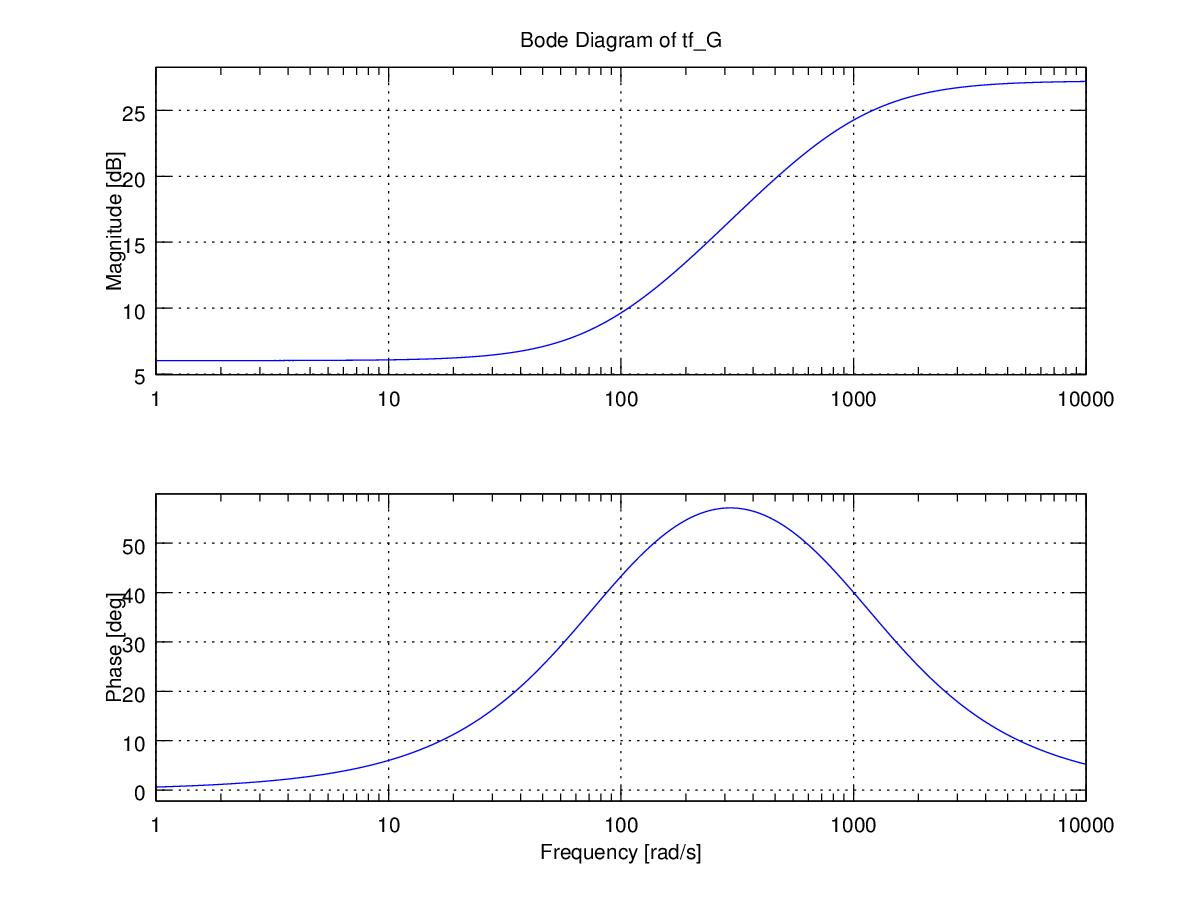
\includegraphics[width=12cm]{UseCaseOpFilter_Bode}
\caption{Default plot for \linnet{} result of kind \code{PLOT}}
\label{figUseCaseOpFilter_Bode}
\end{center}
\end{figure}

\begin{figure}
\begin{center}
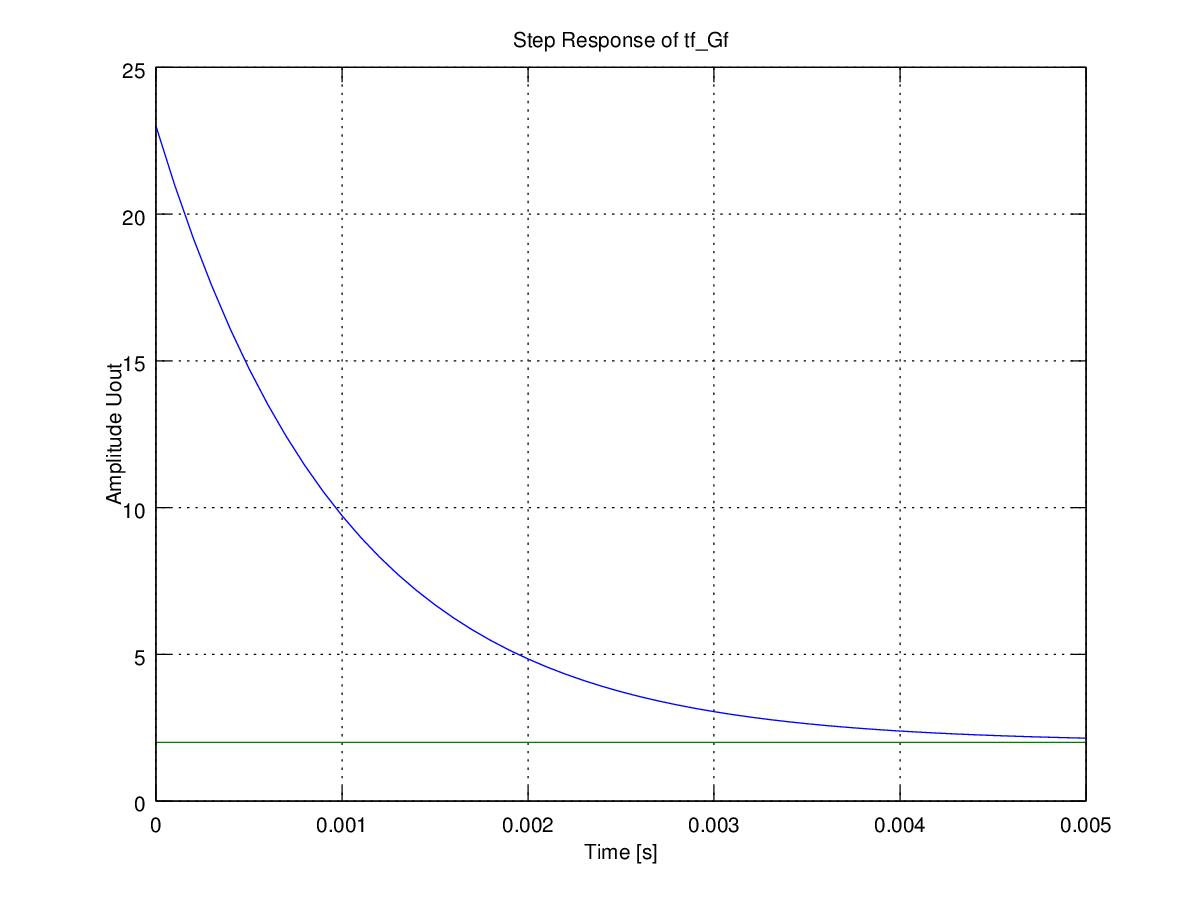
\includegraphics[width=12cm]{UseCaseOpFilter_step}
\caption{Default plot for \linnet{} result of kind \code{RES}}
\label{figUseCaseOpFilter_step}
\end{center}
\end{figure}

Actually, both results are just the same: The filter is a SISO system with
a single input and the full dependency of the output on this input is the
full dependency on \emph{all} inputs at the same time.

Only when looking at the generated Octave code one will recognize a
difference. While the generated LTI object is still identical differs the
default operation performed on this object in both cases. The results have
been implemented as Octave scripts \file{G.m} and \file{Gf.m} in the
output folder \file{opFilter}. If called just like that the default
operation is performed: The Octave command \code{G} opens a figure window
with a Bode plot (see figure \ref{figUseCaseOpFilter_Bode}), command
\code{Gf} presents the plot of the step response (see figure
\ref{figUseCaseOpFilter_step}). Regardless, both Octave scripts can be
applied to produce the same plots and numeric results if you make use of
the optional function parameters and return values. Please, refer to
section \ref{secOctaveInterface} for details.

The next result, which is specified in the netlist file is called
\ident{SIMO}. A full result is demanded for the three quantities
$U_{out}$, $U_{im}$ and $I_{op}$, where $U_{im}$ is the voltage at the
feedback input of the op-amp and $I_{op}$ its output current. \linnet{}
responds with:
\begin{verbatim}
RESULT - User-defined result SIMO:
The solution for unknown Uout:
  Uout(s) = N_Uout_Uin(s)/D_Uout_Uin(s) * Uin(s), with
    N_Uout_Uin(s) = (R1*R2*C1 + R1*R2*C2) * s
                    +(R1 + R2)
    D_Uout_Uin(s) = R1*R2*C1 * s
                    +R2
The solution for unknown U_Im:
  U_Im(s) = N_U_Im_Uin(s)/D_U_Im_Uin(s) * Uin(s), with
    N_U_Im_Uin(s) = 1
    D_U_Im_Uin(s) = 1
The solution for unknown I_OP:
  I_OP(s) = N_I_OP_Uin(s)/D_I_OP_Uin(s) * Uin(s), with
    N_I_OP_Uin(s) = R1*R2*C1*C2 * s^2
                    +(R1*C1 + R2*C2) * s
                    +1
    D_I_OP_Uin(s) = D_Uout_Uin(s)
\end{verbatim}

Again, the found formula for $U_{out}$ is exactly the same. However, this
time it's only one formula out of three, which make up the complete
result. For analytic considerations this is irrelevant. It doesn't matter
if one specifies three single results with \code{RES} or one result with
three dependent quantities. The only important difference can be found in
the generated Octave script: A true SIMO LTI object is created. If typing
\code{tf\_SIMO=SIMO} on the Octave command line all three partial transfer
functions of the SIMO system are printed.

The transfer function $I_{op}(U_{in})$ has a numerator degree in $s$ of
two but a denominator degree of only one, which means that the step
response of the output current has a Dirac impulse; the two capacitors
need to be loaded instantly. Octave can create such an LTI object, see
before, but can't plot the unreal step response; it complains about an
``improper'' system.

The direct capacitive connection of the op-amp's output to ground further
means an infinite output current for high frequencies. This is shown by
the Bode plot Octave presents when typing \code{Iop}, which is the name of
the last user-specified result. The Bode plot of an ``improper'' system
is possible, as long as it is a SISO system. (Octave refuses to draw Bode
plots of SIMO or MIMO systems.)


\subsection{MIMO system}

\linnet{} is not restricted to SISO systems. If more than one independent
sources are in the circuit then we have a multiple input system. \linnet{}
offers to compute all voltages and currents of a circuit, which leads to a
multiple output system. The following use case presents a typical MIMO
scenario.

% Use case MIMO: Analog add
{
% This define is related to the specifics of the array package; see
% http://texwelt.de/wissen/fragen/3401/zentrieren-text-in-tabelle (as of
% July 25 2014) for more
\newcolumntype{M}[1]{>{\centering\arraybackslash}m{#1}}

\begin{figure}
\begin{center}
\begin{tabular}{M{5.5cm}M{6.57cm}}
{\normalsize
\verbatiminput{UseCaseAnalogAdd.cnl}
}
&
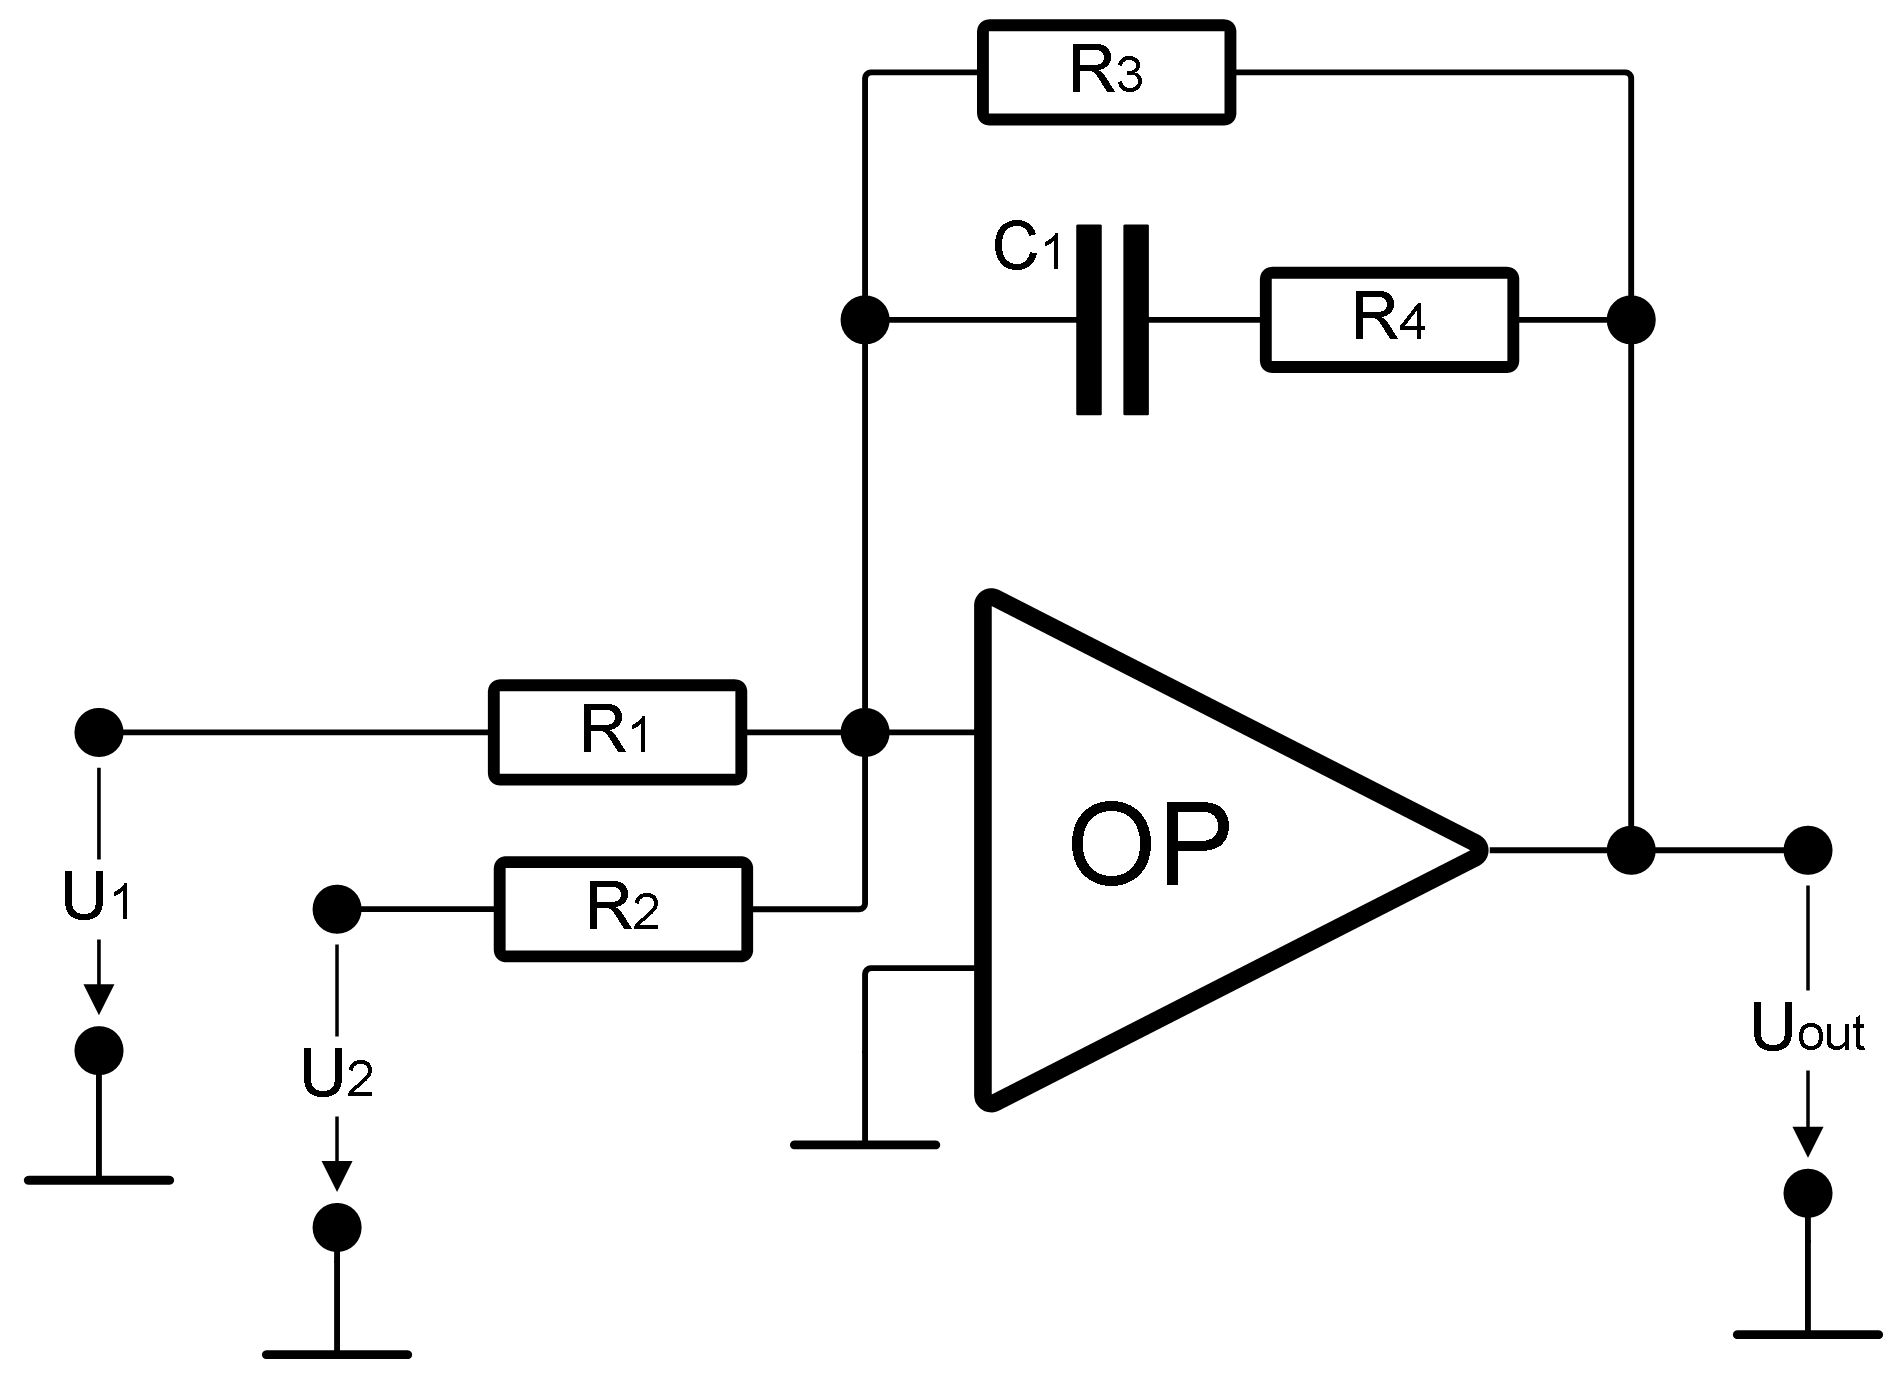
\includegraphics[width=6.57cm]{UseCaseAnalogAdd}
\\

\end{tabular}
\caption{MIMO example: Analog adder}
\label{figUseCaseAnalogAdd}
\end{center}
\end{figure}
} % End of figure for use case MIMO: Analog add

Figure \ref{figUseCaseAnalogAdd} shows an analog adder. The two input
signals are added in a weighted sum in the ratio 1:2. The result
specification \verb+RES MIMO U_out I_OP+ demands two dependents, this
means a MIMO system with two in- and two output. \linnet{} responds with:
\begin{verbatim}
RESULT - User-defined result MIMO:
The solution for unknown U_out:
  U_out(s) = N_U_out_U1(s)/D_U_out_U1(s) * U1(s)
             + N_U_out_U2(s)/D_U_out_U2(s) * U2(s), with
    N_U_out_U1(s) = -4*R1*C1 * s
                    -40
    D_U_out_U1(s) = 41*R1*C1 * s
                    +10
    N_U_out_U2(s) = -8*R1*C1 * s
                    -80
    D_U_out_U2(s) = D_U_out_U1(s)
The solution for unknown I_OP:
  I_OP(s) = N_I_OP_U1(s)/D_I_OP_U1(s) * U1(s)
            + N_I_OP_U2(s)/D_I_OP_U2(s) * U2(s), with
    N_I_OP_U1(s) = -1
    D_I_OP_U1(s) = R1
    N_I_OP_U2(s) = -2
    D_I_OP_U2(s) = R1
\end{verbatim}

The composition of a single result from multiple formulas is already known
from the previous use case, which introduced a SIMO system. Here, the
representation of the multiple inputs is new. Each output is represented
as a sum of two transfer functions, one for each input.

\begin{figure}
\begin{center}
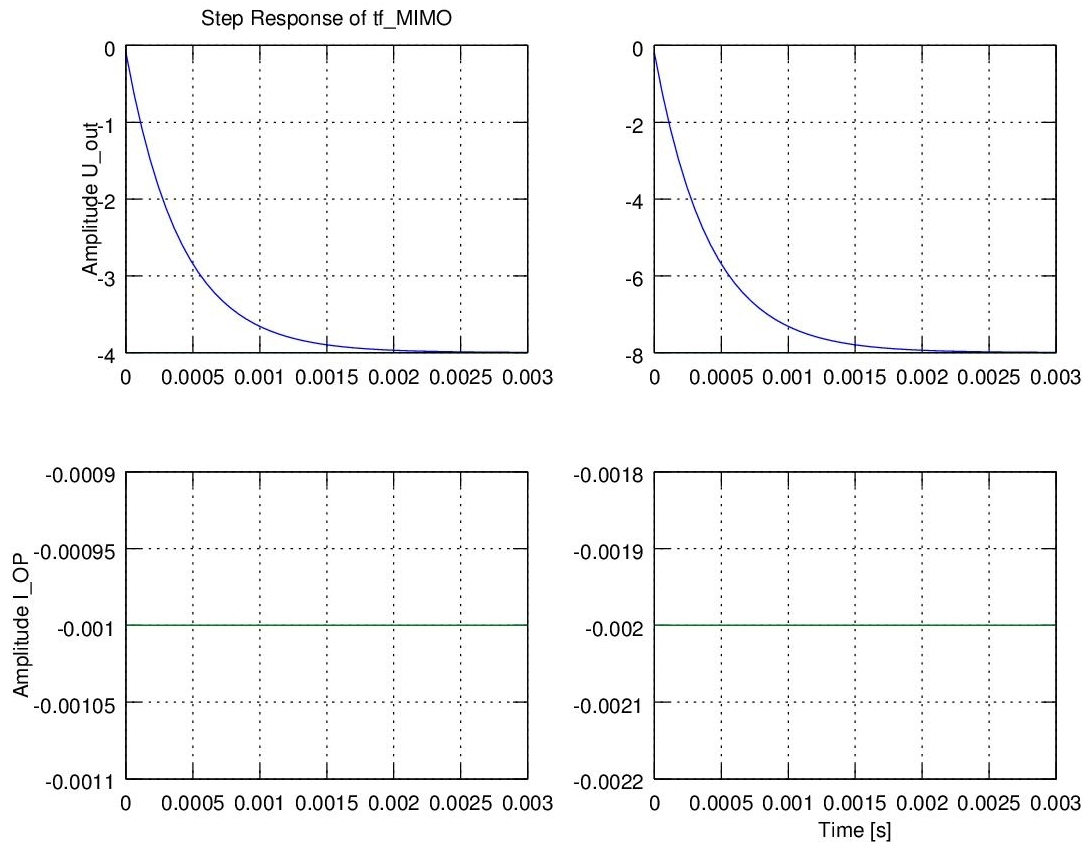
\includegraphics[width=8cm]{UseCaseAnalogAdd_step}
\caption{Step response of MIMO system created with \code{RES}}
\label{figUseCaseAnalogAdd_step}
\end{center}
\end{figure}

The generated Octave script \file{MIMO.m} will plot the step response of
the system, see figure \ref{figUseCaseAnalogAdd_step}. The step response is
presented in a rectangular grid for each in- and output. The meaning of a
single figure is the response of the related output if the related input
undergoes a step and all other inputs are constantly null.

The second user-specified result uses the keyword \code{PLOT}. The
dependency of a single quantity on a single other one is presented as Bode
plot. The result specification \verb+PLOT G1 U_out U1+ yields:
\begin{verbatim}
RESULT - User-defined result G1 (Bode plot):
The dependency of U_out on U1:
  U_out(s) = N_U_out_U1(s)/D_U_out_U1(s) * U1(s), with
    N_U_out_U1(s) = -4*R1*C1 * s
                    -40
    D_U_out_U1(s) = 41*R1*C1 * s
                    +10
\end{verbatim}

\noindent This is not surprisingly one of the partial transfer functions
of the MIMO system. In case of MIMO systems and if Bode plots are wanted
the result kind \code{PLOT} needs to be used to pick out a single partial
transfer function because the Octave command \code{bode} rejects any LTI
object, which doesn't have SISO characteristics.


\section{In- and output impedance of a circuit}

A typical issue in the discussion of an electronic circuit is the in- and
output impedance as a function of the frequency. Since \linnet{} is
capable to figure out all voltages and currents in a linear circuit it is
easily possible to request these functions as a user-defined result.
Please refer to figure \ref{figImpedance}.

% Sample circuit: RLC circuit to demonstrate I/O impedance computation
{
% This define is related to the specifics of the array package; see
% http://texwelt.de/wissen/fragen/3401/zentrieren-text-in-tabelle (as of
% July 25 2014) for more
\newcolumntype{M}[1]{>{\centering\arraybackslash}m{#1}}

\begin{figure}
\begin{center}
\begin{tabular}{M{5.94cm}M{5.06cm}}
{\normalsize
\verbatiminput{impedance.cnl}
}
&
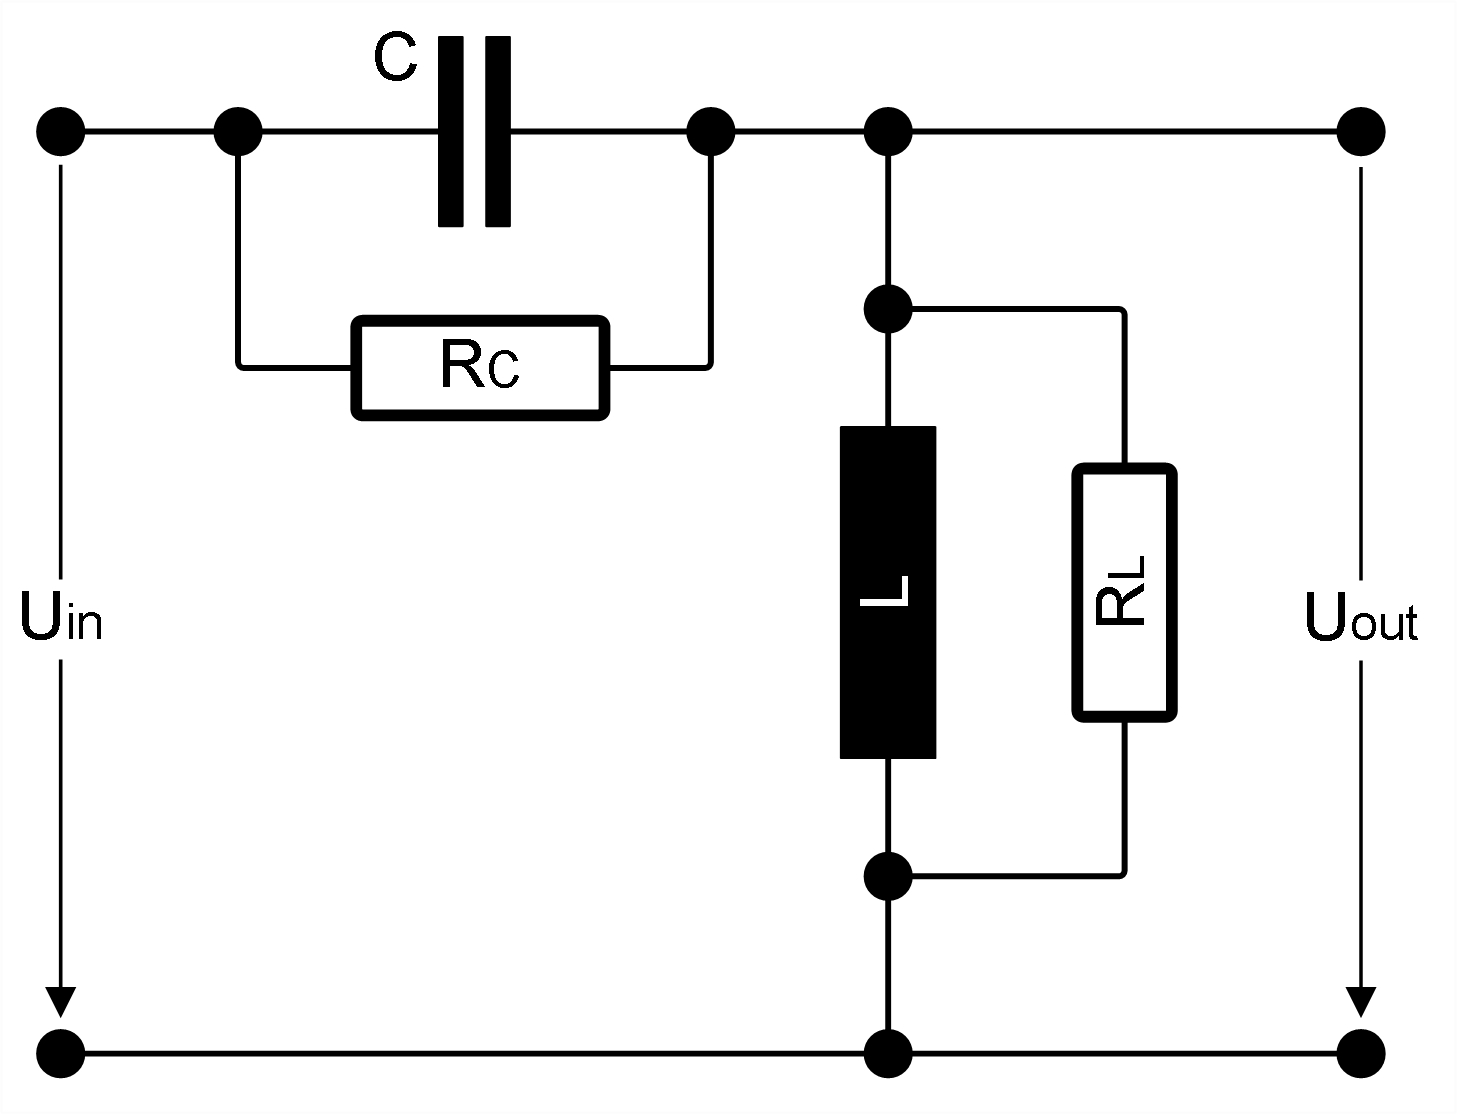
\includegraphics[width=5.06cm]{Impedance}
\\

\end{tabular}
\caption{RLC circuit}
\label{figImpedance}
\end{center}
\end{figure}
} % End of sample circuit: RLC circuit to demonstrate I/O impedance computation


The focus of this use case is put on the definition of the results. The
circuit itself is a simple damped LC resonator.

The user-defined result \ident{G} is the conventional transfer function
from stimulating input voltage $U_{in}$ to resulting output voltage
$U_{out}$. We have already seen this in a previous use case.

The definition of result \ident{Zin} is new. Line \verb+PLOT Zin Uin I_Uin+
requests the transfer function that expresses the dependency of the input
voltage on the input current. The ratio of these two is the input
impedance and we will get it as a function of the signal frequency~$s$. This
function will contain the static DC input impedance as limit $s \to 0$. The
new aspect of this result definition is that the dependent quantity, the
input voltage $U_{in}$, actually is a known quantity to the internal
computation; it's the device constant of the constant voltage source,
which provides the stimulating input voltage. Vice versa, the independent
quantity of the result, the input current $I_{U_{in}}$, is an unknown to the
internal computation. With respect to the internal computation result
\ident{Zin} is the request for an inverse transfer function. \linnet{}
supports inverse transfer functions with the following limitations:
\begin{itemize}
  \item Inverse transfer functions are limited to pairs of two quantities.
    There's no concept of an inverse full result
  \item In MIMO systems one and only one of the two quantities needs to be
    an independent quantity to the internal computation. Or with other
    words: one of the two quantities is a system input
\end{itemize}
The last constraint causes an inconvenience. Usually and like in figure
\ref{figImpedance} the input voltage is connected to a particular node $N$
and the ground node. In which case the voltage potential of node $N$ will
be identical to the input voltage; but regardless of the triviality of
this result it is a dependent quantity to the internal computation. If the
impedance is defined as the dependency of node $N$'s voltage potential on
the input current then this result definition will be invalid for a MIMO
system. As it is natural to name this particular node \code{in} and since
the unknown node potential is addressed to by prefixing this name with
\code{U\_} it becomes a matter of \code{Uin} or \code{U\_in} whether the
result definition is valid or invalid, respectively.

The constraint disappears for SIMO systems: If the system only has a
single input then the relationship between two dependent quantities is well
defined; both follow a modulation of the only input in a certain,
computable way and hence their relationship is known.

In principle, this behavior is natural and easy to understand but it might
be hard to accept due to the in practice typically very similar names of a
voltage source's device constant and the connected node's voltage
potential.

For our example \linnet{} returns:
\begin{verbatim}
RESULT - User-defined result Zin (Bode plot):
The dependency of Uin on I_Uin:
  Uin(s) = N_Uin_I_Uin(s)/D_Uin_I_Uin(s) * I_Uin(s), with
    N_Uin_I_Uin(s) = Rc*Rl*L*C * s^2
                     +(Rc*L + Rl*L) * s
                     +Rc*Rl
    D_Uin_I_Uin(s) = Rc*L*C * s^2
                     +(Rc*Rl*C + L) * s
                     +Rl
\end{verbatim}
The input impedance is the transfer function
\code{N\_Uin\_I\_Uin(s)/D\_Uin\_I\_Uin(s)}. The limit of this function for
$s \to 0$ is $R_C$. For DC operation the capacitor is as not present and
the impedance short-circuits the resistor $R_L$. The remaining resistance
from the input side is $R_C$.

The limit $s \to \infty$ can also be interpreted. The formula yields $R_L$
in this case. For very high frequencies the capacitor short-circuits the
resistor $R_C$ and $L$'s impedance goes against $\infty$. The parallel
resistor $R_L$ is the remaining resistance from the input side.

Between these two ends the magnitude of the complex function has a local
minimum.

If we run the generated Octave script \file{Zin.m} to plot the input
impedance then the standard Bode plot settings are used. Which means that
the $y$ axis is scaled in decibel. For the purpose of an impedance value
maybe not the most convenient convention. To get the values in Ohm
you will have to inverse the dB definition, if you e.g. read a value of
80\,dB in the plot then type \verb+10^(80/20)+ on the Ocatve command
line to get the impedance in Ohm.

Alternatively you can evaluate the generated transfer function for a given
frequency $f$ in Hz. In Octave this is as simple as typing
\code{abs(Zin()(2*pi*f))}.\footnote{In MATLAB the LTI transfer function
objects behave differently; the sample code won't work. You may instead
use function \ident{bode} with parameter $\omega=2 \pi f$ to get the
impedance value at frequency $f$.}

The computation of the output impedance is not that straightforward. It is
defined as the ratio of the output voltage drop caused by an output
current and this current. To put this in \linnet{} manageable terms we
need to extend the circuit by a load. If we use a current source then the
output impedance is the dependency of the output voltage on this load
current. The netlist in figure \ref{figImpedance} already contains a load
current source, see line \verb+I Iload gnd K2+. (Insofar the schematic on
the right hand side of the figure doesn't represent the circuit actually
computed by \linnet{}.)

We define the load current influent to the circuit. A negative voltage
change (a voltage drop) will be caused by a negative current and the
demanded ratio of both will become positive; this is the conventional sign
definition for an output impedance.

Please note, that the extension of the circuit doesn't necessarily need to
be done in a separate step. Other user-defined \code{PLOT} results, e.g.
the transfer function $G$, do not suffer from this additional current
source. If we demanded the full result for the output voltage then we'd
get a changed formula, now with two addends instead of a single term: Each
describing the impact of one of the sources on the output voltage. The
partial transfer function $G$ is just one of these two addends and doesn't
depend on the load current.

The rest holds as for the input impedance. The definition of the output
impedance $Z_{out}$ as \linnet{} result is made in line
\verb+PLOT Zout Uout Iload+. After running \linnet{} you will discuss the found formula:
\begin{verbatim}
RESULT - User-defined result Zout (Bode plot):
The dependency of Uout on Iload:
  Uout(s) = N_Uout_Iload(s)/D_Uout_Iload(s) * Iload(s), with
    N_Uout_Iload(s) = Rc*Rl*L * s
    D_Uout_Iload(s) = Rc*Rl*L*C * s^2
                      +(Rc*L + Rl*L) * s
                      +Rc*Rl
\end{verbatim}
or run the generated Octave script \file{Zout.m} to plot the impedance or
compute its values at particular frequencies. The Octave computations can
be done for particular device values only; these are not configured in
our example netlist and Octave will begin with initial standard values.


\section{Transistor model}

The final use case is the complexest one. Figure \ref{figBipolarTModel}
shows a typical transistor amplifier circuit. The input voltage $U_{in}$
is amplified to the output voltage $U_{out}$. Main characteristics of the
circuit is the frequency response of the output in dependency of the
input. This uses case demonstrates the usage of \linnet{} in the analysis
of such a prototypical circuit.

% Sample circuit: Model of inverting op-amp.
{
% This define is related to the specifics of the array package; see
% http://texwelt.de/wissen/fragen/3401/zentrieren-text-in-tabelle (as of
% July 25 2014) for more
\newcolumntype{M}[1]{>{\centering\arraybackslash}m{#1}}

\begin{figure}
\begin{center}
\begin{tabular}{M{7cm}M{8.3cm}}
{\normalsize
\verbatiminput{BipolarTModel.cnl}
}
&
% The ideal width of the figure to get the same scale of the device as in
% the other schematics would be 8.51cm. This leads to a total width of the
% figure greater than \textwidth. Having a somewhat smaller scale seems to
% be the better choice in this case.
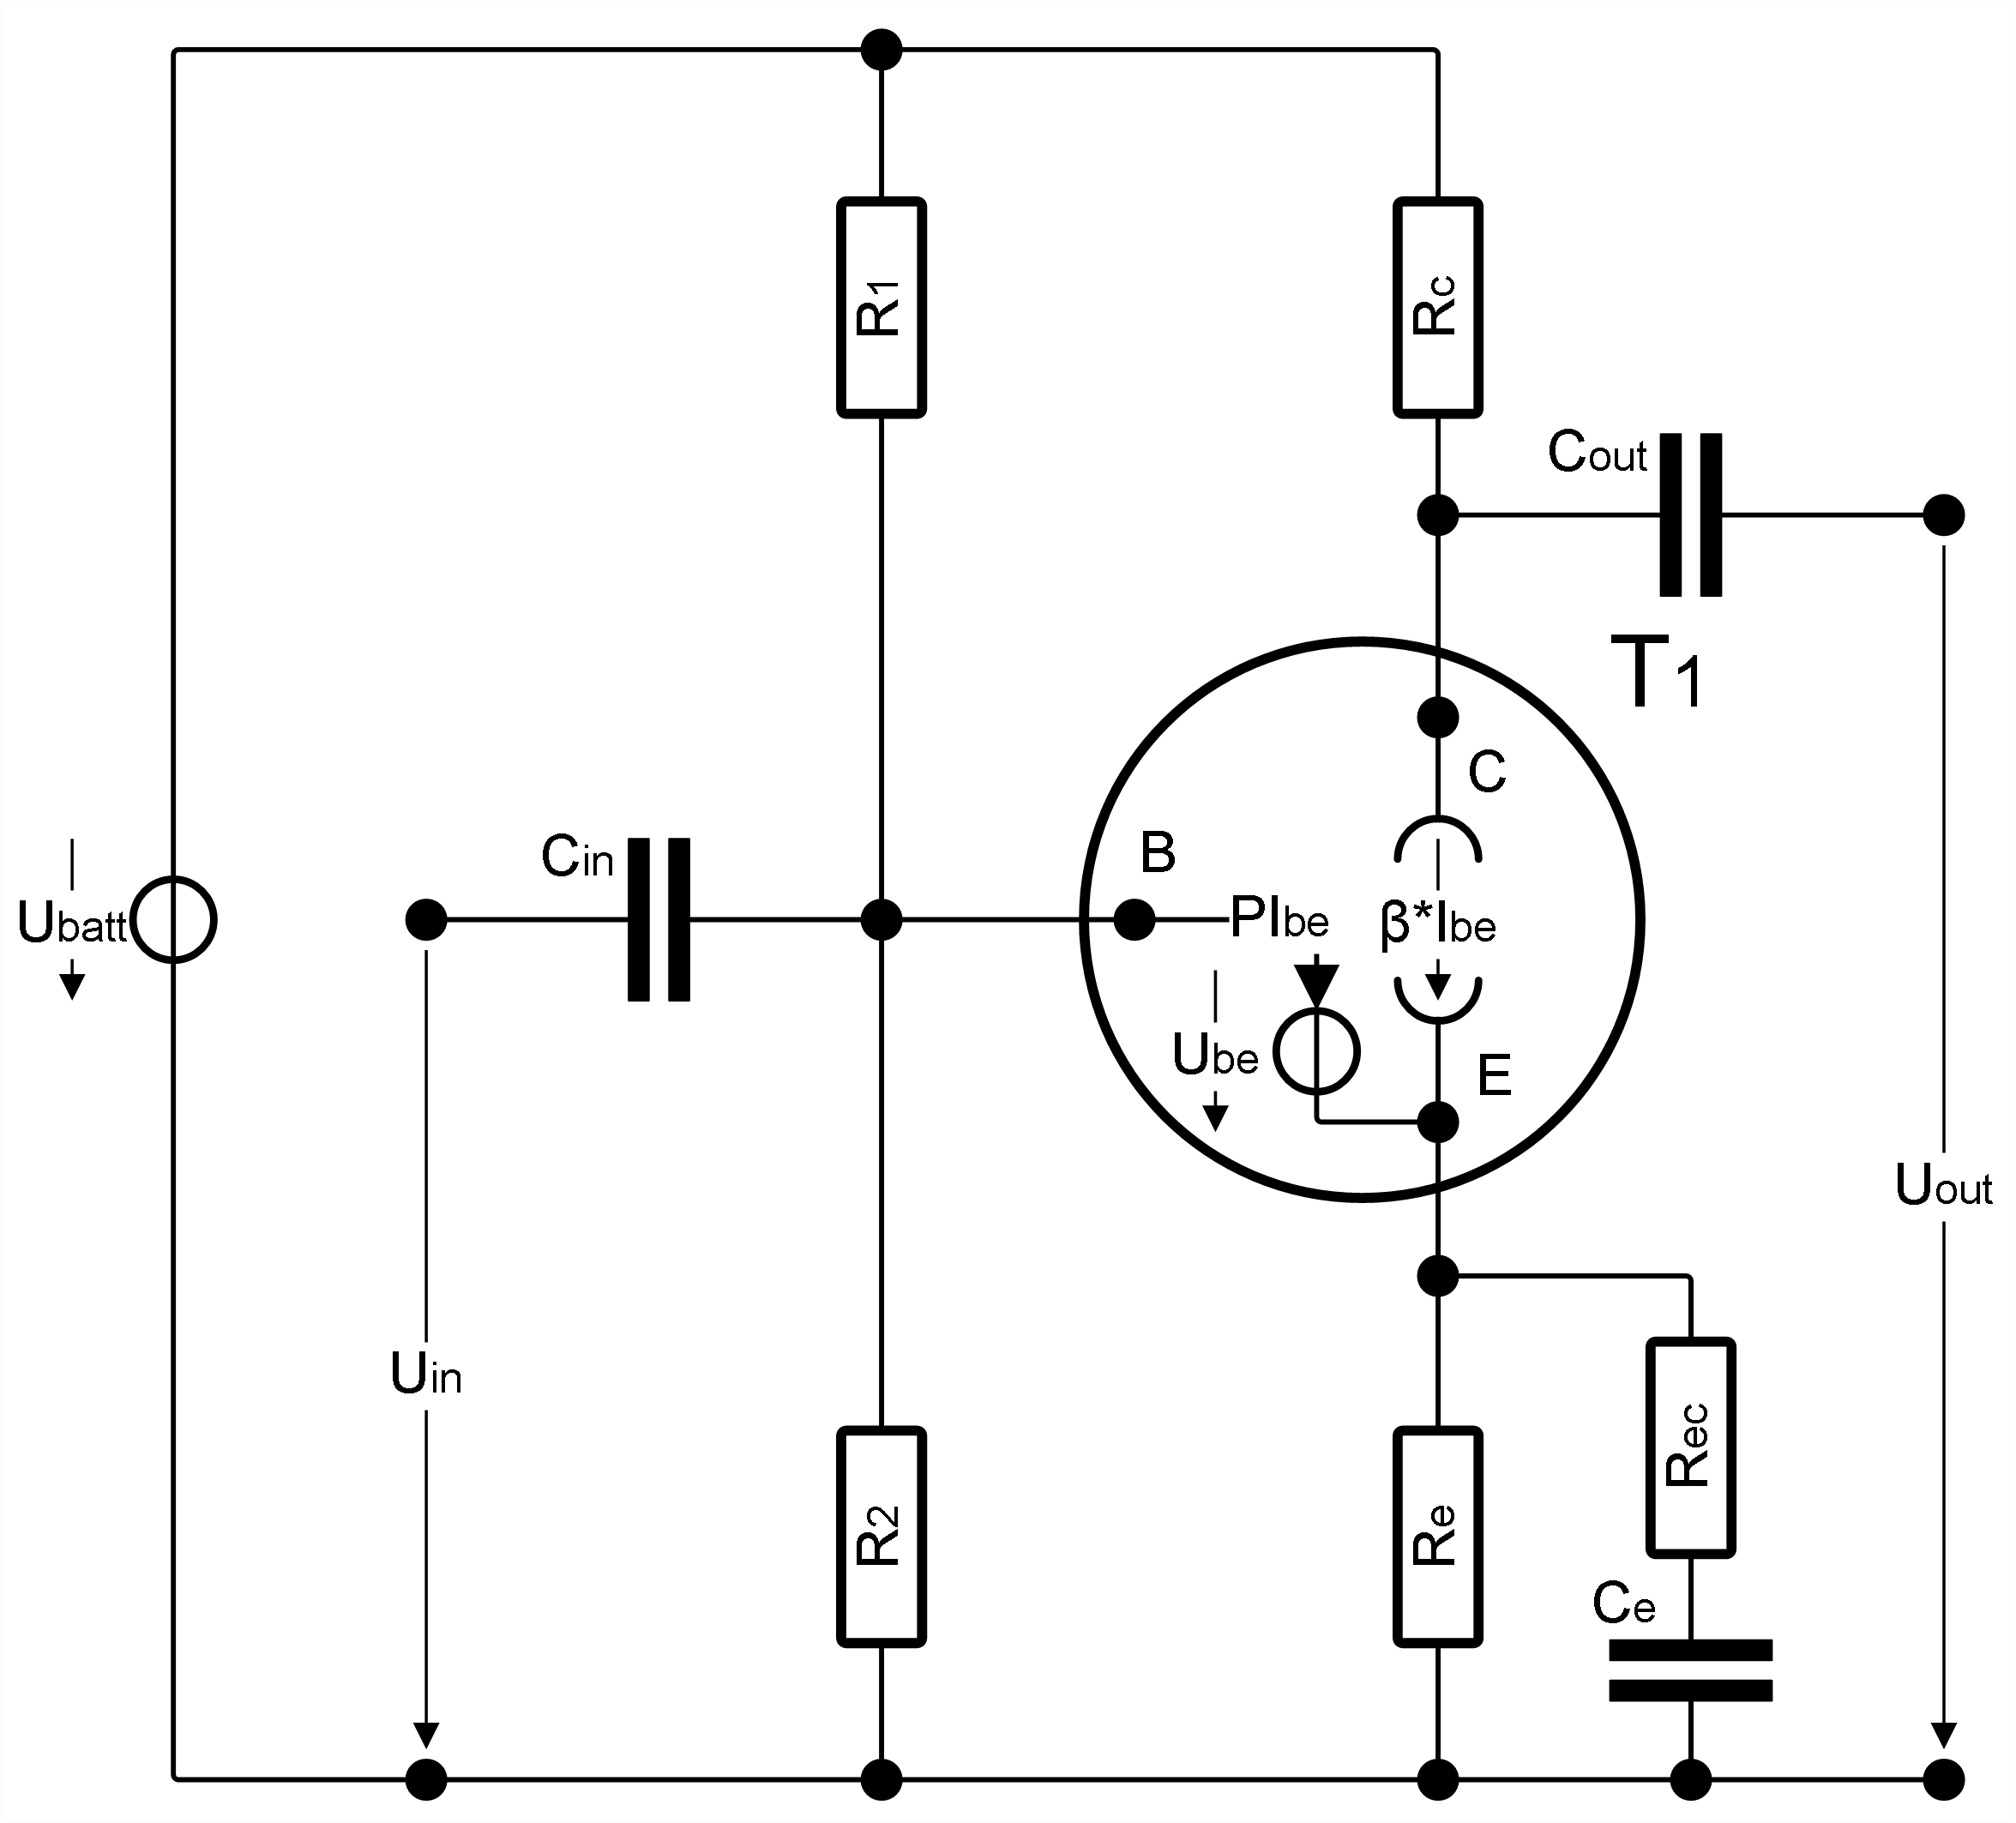
\includegraphics[width=8.3cm]{BipolarTModel}
\\

\end{tabular}
\caption{Bipolar transistor amplifier}
\label{figBipolarTModel}
\end{center}
\end{figure}
} % End of sample circuit: Model of inverting bipolar transistor amplifier.


\subsection{Circuit design}

Initially, a rough calculation is made that leads to an initial set of
numeric device values. The results of the later \linnet{} computation can
then be used to prove the made simplifications and to validate and perhaps
refine the initial findings.

The design of the circuit is driven by some requirements and figured out
based on some simplifications. Let's assume the following requirements:
\begin{itemize}
  \item The amplification should be about 100 or 40\,dB
  \item The output impedance should be in the magnitude of 10\,k$\Omega$
  \item The amplifier should be operational in a frequency range of
    100\,Hz \dots 20\,kHz
  \item The circuit should have a stable operating point
\end{itemize}

The starting point of the design is the yielded amplification. The nominal
current amplification $\beta$ of our transistor be 250. This leaves room
for an emitter current based feedback: The rising voltage at the emitter
resistor due to current amplification will be a counter-control of the
amplification as it directly decreases the base-emitter voltage
drop.\footnote{In the true implementation of the circuit such a feedback
reduces the impact of the non linearity of the real transistor device.
This can't be illustrated, proven or quantified with \linnet{} as
\linnet{} can't model any kind of nonlinearity.}

The emitter voltage nearly follows the input voltage and the current
through the emitter is nearly the current through the collector;
consequently, the expected amplification (disregarding the inversion) is
about the ratio of collector to emitter resistor,
$\left| V \right| \simeq R_c/R_{e_{eff}}$.

A further simplification is that the collector current is relatively
independent of the circuitry in the collector. An hypothetical output
current will therefore always mean an additional voltage drop at $R_c$,
which is proportional to this resistor and the hypothetical current. This
means that the circuit's output impedance has nearly the same value as
$R_c$. According to our requirement we choose a value of $R_c=6.8$\,k, which
means $R_{e_{eff}} \simeq 68\,\Omega$.

The operating point of the collector (i.e. the voltage at input voltage
null) should be somewhat above the middle of the supply voltage to get a
symmetric limit for both polarities of the input voltage. Given $R_c=6.8$\,k
we want to have a collector current
$I_c=5.7\text{\,V}/6.8\text{\,k}\Omega=0.84\text{\,mA}$. It holds
$I_c \simeq I_e$ and accordingly $U_b \simeq U_{be} + R_{e_{eff}} I_c$.
The actual base voltage will be set with the ratio $R_1/R_2$. As $U_{be}$
is considered constant the product $R_{e_{eff}} I_c$ will have to
compensate for any deviation of $U_b$ from the targeted value due to
tolerances of $R_1$ or $R_2$. The larger $R_{e_{eff}}$ the smaller the
deviation of $I_c$ and thus of the targeted operating point.
This consideration explains the emitter circuitry: For DC currents we want
to have a large value to get a stable and targeted operating point but the
design goal $V=100$ already demanded a value of 68\,$\Omega$ for the
relevant input frequency range. The answer is: Place the 68\,$\Omega$ behind
a DC blocking capacitor and put a larger resistor for DC operation in
parallel. We take the tenfold value for DC operation, $R_e=680\,\Omega$;
this won't affect the previous findings too much or with other words,
$R_{e_{eff}}$ for the relevant input frequency range. For DC operation the
effective emitter resistance is $R_e$ and the wanted value for $U_b$ becomes 
$U_b=0.6\text{\,V}+680\text{\,}\Omega \cdot 0.84\text{\,mA}=1.17\text{\,V}$.

The last step of the design is the voltage divider at the transistor's
base. The simplification used here is that the base current can be
neglected in comparison to the currents through the two resistors. This
leads to the simple formula $U_b = R_2/(R_1+R_2) U_{batt}$. Considering
only resistor values from the E12 series (10\% tolerance) we choose 10\,k
and 1.2\,k to get the best fit. The current through the resistors is about
one Milli Ampere, which is a hundredfold of the base current $I_c/\beta$ so
that the made simplification is applicable.


\subsection{Modelling the transistor circuit}
 
Normally a circuit like this is modeled as a so called small-signal
circuit. The true circuit is reduced to those elements, which are relevant
for the frequency response above $f=0$. The resulting circuit would no
longer be operational in a true construction and the DC operating point
can't be computed any longer. In a second step one would then do the
contrary to figure out the DC behavior. Using \linnet{} we can decide to
model all at once.

To \linnet{} the circuit is a system with three independent inputs and a
list of dependent quantities under which our output voltage $U_{out}$. For
us, the two inputs $U_{batt}$ and $U_{be}$ are constant values, we will
have to put the constant values 12\,V and 0.6\,V into the resulting
formulas. However, seeing $U_{batt}$ as a true input signal we can easily
find e.g. the hum suppression of the circuit: Consider $U_{batt}$ had a
frequency component of the public power grid and ask for the transfer
function from power supply to output voltage.

\subsubsection{The transistor model}

The bipolar NPN transistor itself is modeled as an ideal current
amplifier; the collector current is assumed to be $\beta$ times the base
current, where $\beta$ is a constant. It is modeled without
non-linearities and frequency dependencies. To get a full picture of the
DC behaviour the voltage drop from base to emitter is modeled by a
constant voltage source of 0.6\,V.

The current amplification is implemented by a current controlled current
source. The device constant is the factor between the source's current and
the control current. Obviously, the former is the collector current and
the latter the base current. \linnet{} takes a device's name as device
constant in the result representation. Therefore we name the device
\ident{beta}.

The current controlled current source references a current probe to
specify the control current. The probe is placed in series to the base of
the transistor and senses the base current. The name of the probe is
\ident{I\_base} and \linnet{} will use the same name for the sensed
current if it should be referenced from a result definition. (If the
probe's name wouldn't begin with \code{I\_} then \linnet{} would add this
as a prefix in order to make transparent that the referenced quantity is a
current.)


\subsection{The voltage amplification}

The principal characteristics of the transistor circuit is the resulting
amplification, the ratio of magnitudes of out- and input voltage. Due to
the decoupling capacitors we have amplification null for DC. We have to
define the amplification as the voltage ratio at frequencies above the
influence of the capacitors.

We look at the partial result for the output voltage, which only describes
its dependency on the input voltage.

\begin{verbatim}
RESULT - User-defined result G (Bode plot):
The dependency of U_out on Uin:
  U_out(s) = N_U_out_Uin(s)/D_U_out_Uin(s) * Uin(s), with
    N_U_out_Uin(s) = -(beta*R1*R2*Rc*Re*Ce*Cin + beta*R1*R2*Rc*Rec*Ce*Cin) * s^2
                     -beta*R1*R2*Rc*Cin * s
    D_U_out_Uin(s) = (beta*R1*R2*Re*Rec*Ce*Cin + R1*R2*Re*Rec*Ce*Cin) * s^2
                     +(beta*R1*R2*Re*Cin + beta*R1*Re*Rec*Ce + beta*R2*Re*Rec*Ce
                       + R1*R2*Re*Ce + R1*R2*Re*Cin + R1*R2*Rec*Ce + R1*Re*Rec*Ce
                       + R2*Re*Rec*Ce
                      ) * s
                     +(beta*R1*Re + beta*R2*Re + R1*R2 + R1*Re + R2*Re)
\end{verbatim}

Due to our initial considerations we take this result for high input
frequencies, i.e. for high frequencies of $U_{in}$. The amplification $V$
is got as limit $s \to \inf$. We take the quotient of the numerator and
denominator terms of highest power in s:

\begin{eqnarray}
V & = & \lim_{s \to \inf}G(s)
        = - \frac{\beta R_1 R_2 R_c R_e C_e C_{in} + \beta R_1 R_2 R_c R_{ec} C_e C_{in}}
                 {\beta R_1 R_2 R_e R_{ec} C_e C_{in} + R_1 R_2 R_e R_{ec} C_e C_{in}}
        = - \frac{\beta R_c R_e + \beta R_c R_{ec}}{\beta R_e R_{ec} + R_e R_{ec}}
\nonumber \\
  & = & - \frac{\beta}{\beta+1} \frac{R_c}{\frac{R_e R_{ec}}{R_e+R_{ec}}}
\label{eqTAmplification}
\end{eqnarray}

The result (\ref{eqTAmplification}) for the amplification can be
interpreted. $V$ is mainly determined by the second term, which can be
read as the ratio of collector resistor to the parallel circuit of the two
emitter resistors; the emitter capacitor behaves as if not present for
high frequencies.

The earlier made approximation of $V$ as the ratio of the collector
resistor's value and the effective resistance at the emitter was based on
the idea that the same current flew through both resistors and leads to
voltage magnitudes proportional to their values, while due to the constant
$U_{be}$ the voltage drop at the emitter resistor follows the input
voltage. Now we get the corrective first term in
equation~(\ref{eqTAmplification}), which is a number closed to one and
reduces the approximation of the amplification a tiny bit. It expresses
that the currents through emitter and collector are indeed similar but not
identical. The voltage modulation at the collector has to be reduced by
the portion of the base current.

% The content of the next section is double. The same consideration can
% be found in section {In- and output impedance of a circuit}, behind the
% enumeration of the MIMO constraints.
%
% \subsubsection{Important note: Addressing to independent quantities in
% MIMO systems}
% 
% At this point a quite specific and maybe hard to accept behavior of
% \linnet{} will be explained.
% 
% The user-defined Bode result \ident{G} has been requested by the valid
% line
% 
% \verb+PLOT G U_out Uin  LOG 50 10 20k+
% 
% \noindent in the input file. The definition means that voltage potential
% \ident{U\_out} is plotted in dependency of voltage \ident{Uin}. For this
% plot, \ident{Uin} is the independent quantity and \ident{U\_out} the
% dependent quantity. \ident{Uin} refers to the device constant of the
% driving voltage source, which is a known, independent quantity to the
% internal computation.
% 
% The voltage source is connected to nodes \ident{in} and \ident{gnd}. The
% voltage potential of node \ident{in} will become a variable of the
% internal computation. The name of this variable (as explained above) is
% known to be \ident{U\_in}. Since the second connector of the source is the
% ground node it's evident that the voltage potential of this node will be
% identical to the source's constant voltage. The alternative, nearly
% identical line
% 
% \verb+PLOT G U_out U_in  LOG 50 10 20k+
% 
% \noindent
% will however fail to produce a result. To the internal computation
% \ident{U\_in}, the node \ident{in}'s voltage potential, is an unknown,
% dependent quantity -- different to the given source's voltage \ident{Uin}.
% And for MIMO systems it is generally forbidden to request a Bode plot
% where two dependent quantities (with respect to the internal computation)
% depend on each other. If a system has more than a single input than the
% relationship of two dependent quantities is not defined; in general it'll
% differ depending on the input, which is modulated.
% 
% In principle, this behavior is natural and easy to understand but it might
% be hard to accept due to the in practice typically very similar names of a
% voltage source's device constant and the connected node's voltage
% potential.


\subsection{Limits of operational range of transistor}
\label{secTModelOpLimits}

The limitations of the true transistor can't be considered by \linnet{}
(as any non-linearity) and nothing about can be seen in any of the
results.

\begin{figure}
  \centering
  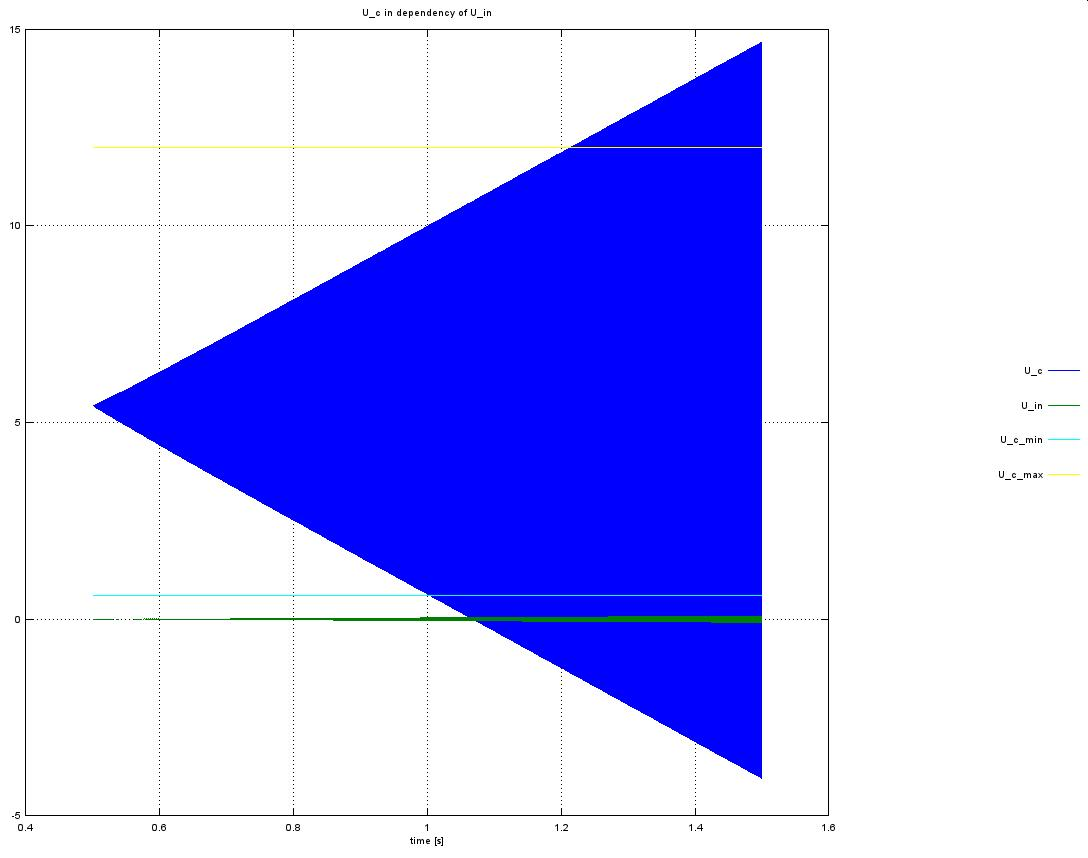
\includegraphics[width=0.7\textwidth]{BipolarTModel_lsim}
  \caption{Simulation of bipolar amplifier circuit in figure
    \ref{figBipolarTModel} with modulated sinoid input
  }
  \label{figBipolarTModel_lsim}
\end{figure}


As an idea to investigate the limits of the amplification we could request
the result for the voltage $U_c$. The true ciruit reaches its limits if
this voltage approaches either $U_{batt}$ or $U_e$ ($U_e$ is nearly
constant by design). In the numeric post-processing with Octave we could
plot this quantity for a rising input signal and compare $U_c$ with
these limits. The point in time, when it first reaches one of the limits
designates the maximum in- and output signal, which could be processed by
a real implementation of the simulated circuit.

This is in one respect a new technique. So far, we focussed on transfer
functions from one quantity to another one. For this investigation we need
to simulate all the inputs since the DC operating point is an essential
part of this computation. Neither the frequency response analysis nor the
step response analysis Ocatve offers will suffice. We need to do a time
domain simulation using all the inputs simultaneously.

An Octave script assembles the required input signal as a 3-column vector
of samples and creates the LTI system object using the \linnet{} generated
result script. Then it runs this system with the input signal. The
simulation result for $U_c$ is shown in figure
\ref{figBipolarTModel_lsim}. At $t=1$\,s the lower limit for $U_c$ is
reached. At this time the input signal has an amplitude of 50\,mV. This is
the maximum input value the true circuit could process without truncation.
The figure shows that the operating point is not yet optimal; both limits
should be reached at the same time to optimally exploit the available
operating range.

The Octave script is printed as listing \ref{lstSimBipolarTModel} on page 
\pageref{secListingOctaveSimulation}. Please refer to this listing to
get more details on how to run a \linnet{} generated LTI system with
arbitrary input signals.

Using a former result, the amplification $V$, another approach is possible.
If we achieved the design goal that the operating point for the collector is
in the center of the possible output voltage range then we can compute the
maximum undistorted peak-peak input voltage by dividing this range by
the found amplification. The found result should nearly be the same as
with the time domain simulation and it would be formula based.

The design goal ``operating point for collector voltage'' can be validated by
demanding the full result for $U_c$ and evaluating the formula for
$U_{in}(s)=0$ and $s=0$. \linnet{} reports for $U_c$:
\begin{verbatim}
RESULT - User-defined result DC:
The solution for unknown U_c:
  U_c(s) = N_U_c_Ubatt(s)/D_U_c_Ubatt(s) * Ubatt(s)
           + N_U_c_Uin(s)/D_U_c_Uin(s) * Uin(s)
           + N_U_c_Ube(s)/D_U_c_Ube(s) * Ube(s), with
    N_U_c_Ubatt(s) = (beta*R1*R2*Re*Rec*Ce*Cin + R1*R2*Re*Rec*Ce*Cin) * s^2
                     +(beta*R1*R2*Re*Cin + beta*R1*Re*Rec*Ce - beta*R2*Rc*Re*Ce
                       - beta*R2*Rc*Rec*Ce + beta*R2*Re*Rec*Ce + R1*R2*Re*Ce
                       + R1*R2*Re*Cin + R1*R2*Rec*Ce + R1*Re*Rec*Ce + R2*Re*Rec*Ce
                      ) * s
                     +(beta*R1*Re - beta*R2*Rc + beta*R2*Re + R1*R2 + R1*Re
                       + R2*Re
                      )
    D_U_c_Ubatt(s) = (beta*R1*R2*Re*Rec*Ce*Cin + R1*R2*Re*Rec*Ce*Cin) * s^2
                     +(beta*R1*R2*Re*Cin + beta*R1*Re*Rec*Ce + beta*R2*Re*Rec*Ce
                       + R1*R2*Re*Ce + R1*R2*Re*Cin + R1*R2*Rec*Ce + R1*Re*Rec*Ce
                       + R2*Re*Rec*Ce
                      ) * s
                     +(beta*R1*Re + beta*R2*Re + R1*R2 + R1*Re + R2*Re)
    N_U_c_Uin(s) = -(beta*R1*R2*Rc*Re*Ce*Cin + beta*R1*R2*Rc*Rec*Ce*Cin) * s^2
                   -beta*R1*R2*Rc*Cin * s
    D_U_c_Uin(s) = D_U_c_Ubatt(s)
    N_U_c_Ube(s) = (beta*R1*R2*Rc*Re*Ce*Cin + beta*R1*R2*Rc*Rec*Ce*Cin) * s^2
                   +(beta*R1*R2*Rc*Cin + beta*R1*Rc*Re*Ce + beta*R1*Rc*Rec*Ce
                     + beta*R2*Rc*Re*Ce + beta*R2*Rc*Rec*Ce
                    ) * s
                   +(beta*R1*Rc + beta*R2*Rc)
    D_U_c_Ube(s) = D_U_c_Ubatt(s)
\end{verbatim}

The operating point for $U_c$ is found as:
\begin{eqnarray}
U_{C0} & = & \frac{(\beta R_1 R_e - \beta R_2 R_c + \beta R_2 R_e + R_1 R_2 + R_1 R_e
                    + R_2 R_e
                   ) U_{batt}
                   + (\beta R_1 R_c + \beta R_2 R_c) U_{be}
                  }
                  {\beta R_1 R_e + \beta R_2 R_e + R_1 R_2 + R_1 R_e + R_2 R_e}
\nonumber \\
       & = & U_{batt} - \frac{\beta R_c}{R_1 R_2 + (1+\beta) (R_1+R_2) R_e}
                        [R_2 U_{batt} - (R_1+R_2) U_{be}]
\label{eqTOperatingPoint}
\end{eqnarray}

Copying the formula (\ref{eqTOperatingPoint}) into Octave and using
$U_{be}=0.6$\,V and $U_{batt}=12$\,V we get $U_{c0}=5.21$\,V.
This is not optimal; taking the constant emitter voltage of about 0.6\,V
into account the ideal value would be about 1\,V higher; a refinement of
the device values can be suggested.

Using Octave we can find out on the fly that the dependency of the
operating point on the transistor amplification $\beta$ is negligible; the
variation $\beta=150 \ldots 300$ yields a variation $U_{c0}=5.26\text{\,V} \ldots
5.20\text{\,V}$.\footnote{The fasted way to reproduce these values is to directly
use the \linnet{} generated LTI object to evaluate the transfer function
at s=0 and to compute the output as linear combination of the three input
contributions:
\verb~
[sys p]=DC;
p.beta=150, sys=DC(p),
F0=sys(0), U\_c0=F0(1,:)*[12; 0; 0.6]~
The first statement is only used to get parameter object \ident{p} that
can then be manipulated for the variation of $\beta$.}
This is important insofar as the transistor amplification has a
high standard deviation for a given device type. A more profound
investigation could even state this as a formula, we can easily figure
out the partial derivative of (\ref{eqTOperatingPoint}) with respect to
$\beta$.

Another aspect: The partial derivatives of (\ref{eqTOperatingPoint}) with
respect to $\beta$ and the resistors would prove whether the trick with
$C_e$ and $R_{ec}$ in parallel circuit to $R_e$ really pays off: it has
been made to reach the design goal for the amplification $V$ without
endangering a stable operating point. If the operating point would however
still be tolerant against typical standard deviations of $\beta$ and the
resistors for a ten times smaller value of $R_e$ then we could live
without this trick.


\subsection{Hum suppression}

The hum suppression might be of interest for a real application of the
circuit if it has a conventional power supply, which might contain some
remains of the 50\,Hz frequency of the public grid. Hum suppression
describes to which extend such remains will be apparent at the circuit
output.

The dependency of the collector voltage $U_c$ on the supply voltage
$U_{batt}$ is part of the user-defined result \ident{DC}, which we had
discussed in the previous section. Even more convenient than evaluating result
\ident{DC} is to specify a result, which is more to the point. Please,
refer to line

\verb+PLOT humSupp U_out Ubatt  LOG 500 10 100+

in the circuit netlist: We demand the dedicated result \ident{humSupp} and
will get an Octave script of same name. The computed formula is exactly
the extract of the full result \ident{DC}, which we need. The default
behavior of the Octave script \file{humSupp.m }is to present the result as
a Bode plot. All we have to do is to run the script and to read the plot
at the frequency of the public power grid. We get a value of only
-0.3\,dB, which means that the hum is propagated to the circuit output
without noticeable damping.

The explanation: In the computation of a MIMO system and if we ask for the
transfer function of one of its inputs to one of its outputs, then the
answer holds under the assumption that the other inputs have given values,
e.g. null all the time (however the actual input function is irrelevant).
With other words its assumed that the inputs are driven with a source of
output impedance null. For our circuit this has the consequence that the
input capacitor $C_{in}$ stabilizes the base voltage of the transistor -
here we have a good hum suppression. Accordingly, the collector current is
also stablized but unfortunately this means that the collector voltage
exactely follows the battery voltage -- and this is what we read from the
Bode plot.

Please note that $C_{out}$ doesn't appear in the transfer function
$U_{batt}$ to $U_{out}$. All computation is ideal and since there's no
load the output capacitor is currentless all time long and hence has no
impact on the output voltage. In any true application of the circuit it
would introduce in conjunction with the input impedance of the following
stage a further time constant in the overall system behavior.


\subsection{Output impedance}

As seen in a previous use case the output impedance of the circuit can be
found by adding a defined load and asking for the dependency of the output
voltage on this load. If we add the lines
\begin{verbatim}
I    Iload gnd   out   
PLOT Zout  U_out Iload LOG 50 10 20k
\end{verbatim}
to the input file then \linnet{} finds a formula of third order in $s$ for
the output impedance. The limit of its value for $s \to 0$ is infinite.
This is expected as the capacitor $C_{out}$ decouples the DC component
from the output signal. The limit for $s \to \infty$ is identical to $R_c$
and in the Bode plot we see that this final value is reached at about
100\,Hz, thus at the beginning of our defined frequency operation range.
This meets our initial expectations.

The picture becomes even clearer if we modify the additional lines in the
input file like this:
\begin{verbatim}
I    Iload gnd c
PLOT Zout  U_c Iload LOG 50 10 20k
\end{verbatim}
Using these lines we actually remove the decoupling output capacitor from
the circuit and define the output impedance at the collector of the
transistor. Now \linnet{} computes the resulting transfer function as:
\begin{verbatim}
RESULT - User-defined result Zout (Bode plot):
The dependency of U_c on Iload:
  U_c(s) = N_U_c_Iload(s)/D_U_c_Iload(s) * Iload(s), with
    N_U_c_Iload(s) = Rc
    D_U_c_Iload(s) = 1
\end{verbatim}
The proportionality factor between current and voltage is identical to the
value $R_c$ of the collector resistor -- this is what we had assumed in
our initial design simplifications.


\appendix
\appendixpage
\addappheadtotoc
\chapter{Formal Syntax Description of Input File}
\label{secBNFOfCnl}

The syntax of the the circuit defining input file (the netlist or
\file{*.cnl} file) in Backus-Naur form:

\begin{small}
\begin{verbatim}
<circuit>       = {[<deviceDef> | <voltageDef> | <resultDef> | <bodeResultDef>] (EOL|';')}
<deviceDef>     = <deviceType> <name> <node> <node> [<node> | <control>] [<relation>]
<deviceType>    = 'R'|'Y'|'C'|'L'|'PI'|'U'[<controlledBy>]|'I'[<controlledBy>]|'OP'
<controlledBy>  = '(' ('U'|'I') ')'
<control>       = <node> <node> | <name>
<relation>      = <name> '=' <quantityRef>
<quantityRef>   = <number> | <deviceRef>
<deviceRef>     = [<rationalNum> '*'] <deviceName>
<voltageDef>    = 'DEF' <name> <node> <node>
<resultDef>     = 'RES' <name> <unknown> {<unknown>} [<plotInfo>]
<bodeResultDef> = 'PLOT' <name> <unknown> <known> [<plotInfo>]
<node>          = <identifier>
<known>         = <name>
<unknown>       = <name>
<name>          = <identifier>
<plotInfo>      = ('LIN' | 'LOG') <integer> <number> <number>
<identifier>    = <character> {<character> | <digit>}
<character>     = 'a' | ... | 'z' | 'A' | ... | 'Z' | '_'
<number>        = <integer> ['.' [<integer>]] [<exponent>]
<rationalNum>   = ['('] <integer> '/' <integer> [')']
<integer>       = <digit> {<digit>}
<exponent>      = ('y' | 'z' | 'a' | 'f' | 'p' | 'n' | 'u' | 'm' | 'c' | 'd'
                   | 'D' | 'h' | 'k' | 'M' | 'G' | 'T' | 'P' | 'X' | 'Z' | 'Y'
                  )
                  | ('E' ['+'|'-'] <integer>)
<digit>         = '0' | ... | '9'
\end{verbatim}
\end{small}

Remarks:

Whitespace separates syntax elements and has not been integrated into
the syntax graph. Blanks and tabs are permitted.

Comments are defined as in C/C++ and are not shown in the syntax graph.

Forward references are generally not supported. This is why result
definitions should appear at the end of the file; they typically refer to
nodes, which need to be already defined. An exception are node references
made in the control inputs of voltage controlled sources; the referenced
nodes may be defined later by being connected to actual devices.

\code{<deviceDef>}: The number of nodes depends:
\begin{itemize}
  \item Most devices have two connectors. They specify two nodes (2 times
    \code{<node>}), which they are connected to
  \item The case having 3 times \code{<node>} is for operational
    amplifiers only
  \item The case having 4 times \code{<node>} is for the voltage
    controlled sources. The first two nodes indicate where the source is
    connected and the second pair (\code{<control>}) defines the
    controlling voltage potential difference
  \item The case having 2 times \code{<node>} followed by a device name
    (\code{<control>}) is for the current controlled sources. The device
    name references an already defined current probe element (type
    \code{PI}). The current through this element is the control current of
    the source
\end{itemize}

\code{<deviceRef>}: \code{<rationalNum>} is a quotient of two positive
integer numbers in the range $[1..999]$. For clarity, the quotient may be
enclosed in parenthesis.

Devices of type \code{U}, \code{I}, \code{OP} and \code{PI} can't have a
value and thus don't have a \code{<relation>}.


Explanation of the specification of the desired computation results:

\code{<voltageDef>}: Definition of any voltage in the network as potential
difference between two nodes. The voltage gets a name.

\code{<resultDef>}: Definition of a full result. Such a result means the
formula how a number of unknowns is composed from all knowns. Named
voltages according to \code{<voltageDef>} and/or any unknown introduced
and named by the LES creator can be referenced. The generated Octave
script code will contain a LTI MIMO transfer function object, which
describes the full set of dependencies between knowns and unknowns.

\code{<bodeResultDef>}: Definition of a frequency response plot. This plot
is limited to the dependency of one quantity on one other one. The result
is implemented as an LTI SISO transfer function object in the generated
Octave script.

\code{<plotInfo>}: The first number is the number of plotted points, in
total for linear frequency axes or per decade for logarithmic axes. The
following pair of numbers is the frequency range.



\chapter{Math}

\section{The elimination method}
\label{secEliminationMethod}

The basic principle of the linear equation system solver is the Gaussian
elimination method. This algorithm replaces a row of coefficients of the
LES with a linear combination of this row and a reference row such that
the leading coefficient of the row becomes a null. Doing this with two
nested loops in an systematic way leads to a triangular matrix of
coefficients, that still represents an equivalent LES and the solution of
the last unknown is already figured out. (The others need additional,
similar operations.) Normally, this algorithm is applied to numerals,
which form an algebraic field. If so, the linear combination of the two
rows is the sum of the reference row times a numeric factor and the row
under progress. To compute this factor the division needs to be defined on
the coefficients and this requires field characteristics.

The symbolic solver operates on a simpler algebraic structure, a ring,
which only knows sum and product but not the division; a prominent example
of this structure are integer numbers.

If we want to apply the Gaussian method to coefficients of a ring than we
have to use another linear combination: Both combined rows are multiplied
crosswise with the leading coefficient of the other row and these two
products are then subtracted. Replacing the row under operation with this
linear combination still fulfills the requirement of shaping null values
in a controlled way and we indeed end up with a triangular matrix and a
solution for the last unknown (and could proceed to figure out the others
as in the standard case).

The problem we face is of purely practical nature: The absolute value of
the coefficients increases in strong exponential order; for our class of
coefficients this would mean an exploding increase of both memory and
computation time. The proposed way out is a known divisor $d$; given $a$
is the coefficient resulting from the previously explained linear
combination then it holds $a = d \tilde a$, where $d$ and $\tilde a$ are
existing instances of the class of coefficients. Since $d$ is identical
for all coefficients of a row we can modify the elimination rule: We
don't replace the row under progress with the results $a$ of the linear
combination so far but with the~$\tilde a$.

The known divisor $d$ is easily computed: it can be found as the last
recently computed coefficient on the diagonal of the matrix and it is one
in the very first iteration.

Some proves are given in this appendix: The main prove confirms the
existance of the factorization $a = d \tilde a$ with the proposed $d$,
which is followed by the proves of particular characteristics of the
coefficients in the given (physical) context, characteristics that
strongly determine the chosen implementation. Finally the correctness and
finiteness of the algorithm that implements the factorization is proven --
either is not apparent from the source code.

Prior to the proves we give an example of the proposed elimination method.


\subsection{Example: Elimination with integer numbers}
\label{secExampleElimMethod}

% Here's some Octave code to prove the presented equations:
% format rat
% LES=[
% -7 ,  3 ,  5 ,  7  , -6  ,  1
%  1 ,  0 , -2 , -5  ,  3  ,  0
%  0 ,  2 ,  0 , -1  ,  13 ,  0
% -3 ,  3 , -7 , -11 ,  8  , -2
% -1 , -2 ,  5 , -3  ,  7  ,  0]
% M = LES(:,1:end-1)
% Y = LES(:,end)
% X=M\Y
% M_Y=LES(:,[1:end-2 end])
% det(M)
% det(M_Y)
%
% Other example, which leads to non cancelled result (can still be cancelled by 9):
% format rat
% LES=[
% -7 ,  3 ,  5 ,  7  , -6  ,  1
%  1 ,  0 , -2 , -5  ,  3  ,  0
%  0 ,  2 ,  0 , -1  ,  13 ,  0
% -4 ,  3 , -7 , -11 ,  8  , -2
% -1 , -2 ,  5 , -3  ,  7  ,  0]
% M = LES(:,1:end-1)
% Y = LES(:,end)
% X=M\Y
% M_Y=LES(:,[1:end-2 end])
% det(M)
% det(M_Y)

Be the following LES given:

\begin{equation}
\label{eqSampleLES}
\left(
\begin{array}{ccccc|c}
$-7$ &  $3$ &  $5$ &  $7$  & $-6$  &  $1$ \\
 $1$ &  $0$ & $-2$ & $-5$  &  $3$  &  $0$ \\
 $0$ &  $2$ &  $0$ & $-1$  &  $13$ &  $0$ \\
$-3$ &  $3$ & $-7$ & $-11$ &  $8$  & $-2$ \\
$-1$ & $-2$ &  $5$ & $-3$  &  $7$  &  $0$
\end{array}
\right)
\end{equation}

\noindent
1st Elimination step, the reference row is the first one, it is combined
with rows 2\ldots5 and the known divisor is $d=1$. The reference row
itself is not touched. This yields:

\begin{displaymath}
\left(
\begin{array}{ccccc|c}
$-7$ &   $3$ &   $5$ &   $7$ &  $-6$ &   $1$ \\
 $0$ &  $-3$ &   $9$ &  $28$ & $-15$ &  $-1$ \\
 $0$ &   $0$ & $126$ & $371$ &  $63$ & $-14$ \\
 $0$ & $-12$ &  $64$ &  $98$ & $-74$ &  $17$ \\
 $0$ &  $17$ & $-30$ &  $28$ & $-55$ &   $1$
\end{array}
\right)
\end{displaymath}

\noindent
2nd elimination step, the reference row is the second one, it is combined
with rows 3\ldots5. The known divisor is the diagonal coefficient of the
1st elimination step, $d=-7$. This yields:

\begin{displaymath}
\left(
\begin{array}{ccccc|c}
$-7$ &  $3$ &   $5$    &    $7$    &  $-6$    &   $1$    \\
 $0$ & $-3$ &   $9$    &   $28$    & $-15$    &  $-1$    \\
 $0$ &  $0$ & $126/-7$ &  $371/-7$ &  $63/-7$ & $-14/-7$ \\
 $0$ &  $0$ & $-84/-7$ &   $42/-7$ &  $42/-7$ & $-63/-7$ \\
 $0$ &  $0$ & $-63/-7$ & $-560/-7$ & $420/-7$ &  $14/-7$
\end{array}
\right) =
\end{displaymath}

\begin{displaymath}
\left(
\begin{array}{ccccc|c}
$-7$ &  $3$ &   $5$ &   $7$ &  $-6$ &  $1$ \\
 $0$ & $-3$ &   $9$ &  $28$ & $-15$ & $-1$ \\
 $0$ &  $0$ & $-18$ & $-53$ &  $-9$ &  $2$ \\
 $0$ &  $0$ &  $12$ &  $-6$ &  $-6$ &  $9$ \\
 $0$ &  $0$ &   $9$ &  $80$ & $-60$ & $-2$
\end{array}
\right) \\
\end{displaymath}

\noindent
3rd elimination step, the reference row is the third one, it is combined
with rows 4 and 5. The known divisor is the diagonal coefficient of the
second elimination step, $d=-3$. This yields:

\begin{displaymath}
\left(
\begin{array}{ccccc|c}
$-7$ &  $3$ &   $5$ &    $7$    &   $-6$    &    $1$    \\
 $0$ & $-3$ &   $9$ &   $28$    &  $-15$    &   $-1$    \\
 $0$ &  $0$ & $-18$ &  $-53$    &   $-9$    &    $2$    \\
 $0$ &  $0$ &   $0$ &  $744/-3$ &  $216/-3$ & $-186/-3$ \\
 $0$ &  $0$ &   $0$ & $-963/-3$ & $1161/-3$ &   $18/-3$
\end{array}
\right) =
\end{displaymath}

\begin{displaymath}
\left(
\begin{array}{ccccc|c}
$-7$ &  $3$ &   $5$ &    $7$ &   $-6$ &  $1$ \\
 $0$ & $-3$ &   $9$ &   $28$ &  $-15$ & $-1$ \\
 $0$ &  $0$ & $-18$ &  $-53$ &   $-9$ &  $2$ \\
 $0$ &  $0$ &   $0$ & $-248$ &  $-72$ & $62$ \\
 $0$ &  $0$ &   $0$ &  $321$ & $-387$ & $-6$
\end{array}
\right) \\
\end{displaymath}

\noindent
Last elimination step, the reference row is the fourth one, it is combined
with row 5. The known divisor is the diagonal coefficient of the
third elimination step, $d=-18$. This yields:

\begin{displaymath}
\left(
\begin{array}{ccccc|c}
$-7$ &  $3$ &   $5$ &    $7$ &      $-6$            &       $1$           \\
 $0$ & $-3$ &   $9$ &   $28$ &     $-15$            &      $-1$           \\
 $0$ &  $0$ & $-18$ &  $-53$ &      $-9$            &       $2$           \\
 $0$ &  $0$ &   $0$ & $-248$ &     $-72$            &      $62$           \\
 $0$ &  $0$ &   $0$ &    $0$ & $119088/-18=-6616$ & $-18414/-18=1023$
\end{array}
\right)
\end{displaymath}

\noindent
The solution for the last unknown is $1023/-6616$. The coefficients of the
last row of the last elimination step designate the determinants of the
LES (i.e. the main determinant and the one related to the unknown
according to Cramer's rule):

\begin{displaymath}
\left|
\begin{array}{ccccc}
$-7$ &  $3$ &  $5$ &  $7$  & $-6$  \\
 $1$ &  $0$ & $-2$ & $-5$  &  $3$  \\
 $0$ &  $2$ &  $0$ & $-1$  &  $13$ \\
$-3$ &  $3$ & $-7$ & $-11$ &  $8$  \\
$-1$ & $-2$ &  $5$ & $-3$  &  $7$
\end{array}
\right| = -6616
\end{displaymath}

\begin{displaymath}
\left|
\begin{array}{ccccc}
$-7$ &  $3$ &  $5$ &  $7$  &  $1$ \\
 $1$ &  $0$ & $-2$ & $-5$  &  $0$ \\
 $0$ &  $2$ &  $0$ & $-1$  &  $0$ \\
$-3$ &  $3$ & $-7$ & $-11$ & $-2$ \\
$-1$ & $-2$ &  $5$ & $-3$  &  $0$
\end{array}
\right| = 1023
\end{displaymath}


\subsection{Prove of statement about known divisor}

The prove of the statement that we can find a common divisor in each
elimination step as the diagonal coefficient of the previous elimination
step is based on some algebraic transformations, which will show that
after the elimination step each coefficient has the meaning of the
determinant of a sub-matrix of the LES. Due to the Laplace expansion of a
determinant, which computes the determinant only with products and sums,
this must be an existing element of the class of coefficients.

% @{}: Discard indentation of before and/or behind columns
\medskip
\noindent
\begin{tabular}{p{0.91\textwidth}r}
Definition: Be $M^{[k]}_{m n}$ the sub-matrix of $M$, which
has the dimension $k \times k$ and the coefficients $a_{ij}$ of $M$ at
$i=1..k-1,m$ and $j=1..k-1,n$ with $m, n \geq k$.
& \eqnum \label{eqDefSubMatrix} \\
\end{tabular}
\smallskip

\noindent
$M^{[k]}_{m n}$ is a square matrix. It inherits the upper-left
square of $M$ and has one additional row that has the
coefficients of row $m$ of $ M$ and one additional column that
has the coefficients of row $n$ of $M$.

Examples: If $M$ is the matrix (\ref{eqSampleLES}) from the example
in section \ref{secExampleElimMethod} then we have $M^{[1]}_{1 4}=7$,
\begin{displaymath}
M^{[2]}_{2 3} =
\left(
\begin{array}{cc}
-7 &   5 \\
 1 &  -2
\end{array}
\right)
\end{displaymath}
or
\begin{displaymath}
M^{[4]}_{4 6} =
\left(
\begin{array}{cccc}
-7 &  3 &  5 &  1 \\
 1 &  0 & -2 &  0 \\
 0 &  2 &  0 &  0 \\
-3 &  3 & -7 & -2
\end{array}
\right)
\end{displaymath}

% @{}: Discard indentation of before and/or behind columns
\medskip
\noindent
\begin{tabular}{p{0.91\textwidth}r}
Lemma: Be $M$ the representation of a LES of dimension $p \times q$ with
$q \geq p$ and $M^{(k)}$ with $k=1 \ldots p-1$ the result of elimination
step $k$ of the proposed elimination method and $a^{(k)}_{m n}$ the
coefficient of $M^{(k)}$ at position $mn$. It holds:
\begin{equation*}
a^{(k)}_{m n} = \left|M^{[k+1]}_{m n}\right| \qquad \text{with } m,n > k
\end{equation*}
& \eqnum \label{eqLemmaCoefIsDet} \\
\end{tabular}
\smallskip

\noindent
Lemma (\ref{eqLemmaCoefIsDet}) is what we still have to prove: If we know
that the resulting coefficients are determinants of sub-matrices of the
original, the LES describing matrix $M$ then it must be existing
valid instances from the class of coefficients and the factorization was
possible. 

The prove of lemma (\ref{eqLemmaCoefIsDet}) is given for a particular
coefficient $a_{ij}$ of the LES. We have to consider the position of the
coefficient in the matrix and and the elimination step. The elimination
step is denoted by the top index in parenthesis. The original LES is
represented by matrix $M^{(0)}$. (Elimination step 0 means prior to the
first elimination step. $M^{(0)}$ is also simply written as $M$ -- the
explicit indication of elimination step 0 is mostly omitted.) The lemma
relates the coefficient $a^{(k)}_{ij}$ that is the result of elimination
step $k$ with the determinant of a particular, square sub-matrix of
$M^{(0)}$. The idea of the prove is to look at the coefficients of $M^{(0
\ldots k)}$ at the positions that belong to this sub-matrix and to keep
track what the operations of the eliminations steps mean to the value of
the determinant of the sub-matrix. This leads to a chained equation, which
finally proves the lemma. (Opposed to the relation of the $M^{(0 \ldots
k)}$, which is an equivalence of LESs.) This looking at the coefficients
of the sub-matrix means to reduce the prove for any elimination step of
any rectangular matrix to the final elimination result of a square
matrix.


\subsection{Reducing the problem to square matrices}
\label{secReduceToSqMat}

It is essential that all the sub-matrices $M^{[1 \ldots n](0)}_{ij}$ in
question are square and that they share the upper-left square area of $M$.
All the factors of the linear combinations of rows to be computed are
derived only from the coefficients found in this shared area and therefore
the linear combinations made on the rows of the LES are always the same as
one would have to use to perform the elimination of only the sub-matrix or
of its determinant. This is now illustrated with an example:

Be $M$ the matrix, which represents a LES with 5 unknowns and 2
knowns:
\begin{equation}
M=\left(
\begin{array}{ccccc:cc}
a_{11} & a_{12} & a_{13} & a_{14} & a_{15} & a_{16} & a_{17} \\
a_{21} & a_{22} & a_{23} & a_{24} & a_{25} & a_{26} & a_{27} \\
a_{31} & a_{32} & a_{33} & a_{34} & a_{35} & a_{36} & a_{37} \\
a_{41} & a_{42} & a_{43} & a_{44} & a_{45} & a_{46} & a_{47} \\
a_{51} & a_{52} & a_{53} & a_{54} & a_{55} & a_{56} & a_{57} \\
\end{array}
\right)
\end{equation}

\noindent
Let's take the coefficient at row 5, column 4: The lemma says

\begin{equation*}
a^{(1)}_{54} = \left| M^{[2]}_{54} \right| =
\left|
\begin{array}{cc}
a_{11} & a_{14} \\
a_{51} & a_{54}
\end{array}
\right|
\end{equation*}

\noindent
When the first iteration of the elimination of the matrix $M$ reaches the
last row it replaces:

\begin{equation*}
R^{(1)}_{5} = a_{11} R^{(0)}_{5} - a_{51} R^{(0)}_{1} \text{,}
\end{equation*}

\noindent
which is -- for the affected four coefficients shared between $M$ and
$M^{[2]}_{54}$ -- exactly the same operation as an elimination of
$M^{[2]}_{54}$ would be:

\begin{equation*}
M^{[2](1)}_{54} =
\left(
\begin{array}{cc}
a_{11} & a_{14} \\
0      & a_{11} a_{54} - a_{51} a_{14}
\end{array}
\right)
\end{equation*}

\noindent
All other operations of the first iteration of the
elimination on $M$ affect rows and columns outside of $M^{[2]}_{54}$ and have no
impact on any of the coefficients of $M^{[2](1)}_{54}$.

Or let's take the coefficient at row 4, column 6: The lemma says

\begin{equation*}
a^{(2)}_{46} = \left| M^{[3]}_{46} \right| =
\left|
\begin{array}{ccc}
a_{11} & a_{12} & a_{16} \\
a_{21} & a_{22} & a_{26} \\
a_{41} & a_{42} & a_{46}
\end{array}
\right|
\end{equation*}

\noindent
(Please note, that this example refers to a coefficient,
which has not the final value of the complete elimination, there will also
be the value $a^{(3)}_{46}$ during further processing.)

In the first elimination step and when the process reaches rows 2 and 4
then shared coefficients are touched. The factors of the linear
combination of rows ($(a_{11}, a_{21})$ and $(a_{11}, a_{41})$ for rows 2
and 4, respectively) are located at according positions in $M$ and
$M^{[3]}_{46}$ (i.e. in the first column) and thus the elimination of $M$
is exactly the same operation as seen in its sub-matrix $M^{[3]}_{46}$.
For both matrices the identical row replacements

\begin{eqnarray*}
R^{(1)}_{2} &=& a_{11} R^{(0)}_{2} - a_{21} R^{(0)}_{1} \\
R^{(1)}_{4} &=& a_{11} R^{(0)}_{4} - a_{21} R^{(0)}_{4}
\end{eqnarray*}

\noindent
take place (using the same global position indices in the matrix
representations).

If we look at the second elimination step it's just the same: the operation
performed on the rows of matrix $M^{(1)}$ is

\begin{equation*}
R^{(2)}_{i} = a^{(1)}_{22} R^{(1)}_{i} - a^{(1)}_{i2} R^{(1)}_{2}
\qquad \text{with } i=3 \ldots 5
\end{equation*}

\noindent
Coefficients, which are shared with the sub-matrix are affected only for
$i=4$ and then we see the same operation on the coefficients of the
sub-matrix that would be used to run the second elimination step directly
on the isolated sub-matrix. The required factors $(a^{(1)}_{22},
a^{(1)}_{42})$ of the linear combination are found at the appropriate
position in the sub-matrix.

This idea holds in general for all sub-matrices in question because they
all share their $k-1$ top-most rows and left-most columns with the
original matrix $M$ and the factors of all the linear combinations are
taken from these rows and columns - be it the original coefficients or the
products of the $k-2$ involved, first elimination steps.

This is why we can now reduce the prove to the elimination of the square
sub-matrices. We have to show that the final value of the bottom-right
coefficient in the square area is identical to the determinant of the
original sub-matrix. This result for a particular but arbitrary
coefficients can then be applied to any coefficient computed in any
elimination step.

But before we can start with the prove we need to introduce a minor lemma,
which is applied in the following.


\subsection{Linear combination of rows of determinant}

For the following steps we need to understand how the value of the
determinant of a square matrix is changed if a row of the matrix is
replaced by the linear combination of itself and another row.

% @{}: Discard indentation of before and/or behind columns
\medskip
\noindent
\begin{tabular}{p{0.91\textwidth}r}
Lemma: Be $M$ a square matrix and $\hat M$ the same matrix, where only row
$R_j$ has been replaced with the linear combination $c_j R_j +
c_i R_i$ of this row and the other row $R_i$. It holds: $|\hat M|=c_j
|M|$.
& \eqnum \label{eqLemmaLinCombRowsD} \\
\end{tabular}
\smallskip

\noindent
To prove lemma (\ref{eqLemmaLinCombRowsD}) we just need to expand $|\hat
M|$ along its row $j$:

% =
%c_j \left|
%\begin{array}{ccc}
%a_{11} & \ldots & a_{1n} \\
%\vdots & \ddots & \vdots \\
%a_{n1} & \ldots & a_{nn}
%\end{array}
%\right| =
%c_j \left| M \right|

\begin{eqnarray}
\left| \hat M \right| & = &
\left|
\begin{array}{ccc}
a_{11}                  & \ldots & a_{1n} \\
\vdots                  &        & \vdots \\
a_{i1}                  & \ldots & a_{in} \\
\vdots                  &        & \vdots \\
c_j a_{j1} + c_i a_{i1} & \ldots & c_j a_{jn} + c_i a_{in} \\
\vdots                  &        & \vdots \\
a_{n1}                  & \ldots & a_{nn}
\end{array}
\right| \nonumber \\
  & = & \sum^{n}_{c=1}(-1)^{i+c} (c_j a_{jc} + c_i a_{ic}) D_{jc}
\qquad \text{with } D_{ij} \text{ being the sub-determinant at position } ij \nonumber \\
  & = & c_j \sum^{n}_{c=1}(-1)^{i+c} a_{jc} D_{jc}
        + c_i \sum^{n}_{c=1}(-1)^{i+c} a_{ic} D_{jc} \label{eqProveLemmaLinCombRowsD} \\
  & = & c_j \left| M \right| + c_i \cdot 0 \nonumber
\end{eqnarray}

\noindent
Both determinants in lemma (\ref{eqLemmaLinCombRowsD}), $|M|$ and $|\hat
M|$, share all rows but row $j$, hence all sub-determinants $D_{jc}, c=1
\ldots n$ are identical for both. Therefore the sum in the first addend in
(\ref{eqProveLemmaLinCombRowsD}) is the Laplace expansion of the
determinant of $M$. The sum in the second addend in
(\ref{eqProveLemmaLinCombRowsD}) is null; it is the Laplace expansion of a
similar determinant: all rows but $j$ are identical but row $j$ is
replaced by row $i$. The determinant of a matrix with two identical thus
linear dependent rows is null. Equation (\ref{eqProveLemmaLinCombRowsD})
reduces to lemma (\ref{eqLemmaLinCombRowsD}).

% Determinant with identical rows is null: Swap two rows: Expansion
% according to sum of all permutated tupels proves that the sign of the
% determinant is inverted. If these rows are identical then the
% determinant has not changed at all, so the value is unchanged. This can
% only hold for the particular value null.


\subsection{Prove for square sub-matrix}

From now on we take the view at the sub-matrix only. To simplify the
explanations we change the position indices of the coefficients. We are
going to use consecutive one based indices as usual. The positional
relationship with the matrix of the LES might be obscured but is out of
scope in this section anyway.

We investigate the elimination of an arbitrary square sub-matrix $S$
according to definition (\ref{eqDefSubMatrix}) of $M$, the matrix describing
the original LES:

\begin{eqnarray*}
S^{(0)} & = & M^{[n](0)}_{ij}\qquad \text{with } n>1, i \geq n, j \geq n \\
        & = &
\left(
\begin{array}{ccc}
a_{11} & \ldots & a_{1n} \\
\vdots & \ddots & \vdots \\
a_{n1} & \ldots & a_{nn}
\end{array}
\right) \qquad \text{(here using the renamed position indices)}
\end{eqnarray*}

\noindent
and define $D$ to be its determinant:

\begin{eqnarray*}
D & := & \left| S^{(0)} \right| \\
  & =  &
\left|
\begin{array}{ccc}
a_{11} & \ldots & a_{1n} \\
\vdots & \ddots & \vdots \\
a_{n1} & \ldots & a_{nn}
\end{array}
\right|
\end{eqnarray*}

\noindent
Please note that due to the redefinition of the position indices $a_{ij}$
no longer is the coefficient of $M$ in row $i$ and column $j$ if either
$i=n$ or $j=n$.

After the first elimination step of the LES -- and according to section
\ref{secReduceToSqMat} the first elimination step of $S$ -- the matrix and
its determinant change as follows:

\begin{eqnarray}
S^{(1)} & = &
\left(
\begin{array}{cccc}
a_{11} & \ldots       &           & a_{1n}       \\
0      & a^{(1)}_{22} & \ldots    & a^{(1)}_{2n} \\
\vdots & \vdots       & \ddots    & \vdots       \\
0      & a^{(1)}_{n2} & \ldots & a^{(1)}_{nn}
\end{array}
\right) \nonumber \\
D^{(1)} & := & \left| S^{(1)} \right|                                 \nonumber \\
        & =  & \frac{\left(a_{11}\right)^{(n-1)}}{1^{(n-1)}} \left| S(0) \right| \nonumber \\
        & =  & \frac{\left(a_{11}\right)^{(n-1)}}{1^{(n-1)}} D \label{eqSqrMatD1}
\end{eqnarray}

\noindent
The factor in front of $D$ in equation (\ref{eqSqrMatD1}) is explained by
the $n-1$ row operations that form the elimination step: The rows $2
\ldots n$ are all multiplied by $a_{11}$ as part of the linear combination
with the first row, which explains according to lemma
(\ref{eqLemmaLinCombRowsD}) the numerator of the factor. Then the rows are
all divided by the common divisor, which is one in the first elimination
step. This explains the denominator of the factor.

If we now present the second elimination step, too, then a general pattern
becomes apparent, which gives us the wanted result for any size of matrix
and its determinant:

\begin{eqnarray}
S^{(2)} & = &
\left(
\begin{array}{ccccc}
a_{11} & \ldots       &              &        & a_{1n}       \\
0      & a^{(1)}_{22} & \ldots       &        & a^{(1)}_{2n} \\
0      & 0            & a^{(2)}_{33} & \ldots & a^{(2)}_{3n} \\
\vdots & \vdots       & \vdots       & \ddots & \vdots       \\
0      & 0            & a^{(2)}_{n3} & \ldots & a^{(2)}_{nn}
\end{array}
\right) \qquad \text{with }
a^{(2)}_{ij} = \frac{a^{(1)}_{22} a^{(1)}_{ij} - a^{(1)}_{i2} a^{(1)}_{2j}}{a_{11}} \\
\nonumber \\
D^{(2)} & = & \frac{\left(a^{(1)}_{22}\right)^{(n-2)}}{(a_{11})^{(n-2)}} D^{(1)} \nonumber \\
        & = & \frac{\left(a^{(1)}_{22}\right)^{(n-2)}}{(a_{11})^{(n-2)}}
              \frac{\left(a_{11}\right)^{(n-1)}}{1^{(n-1)}} D                    \nonumber \\
        & = & (a^{(1)}_{22})^{(n-2)} a_{11} D \label{eqSqrMatD2}
\end{eqnarray}

\noindent
The pattern: In elimination step $k$ we multiply $n-k$ rows with the
value $v = a^{(k-1)}_{kk}$, which temporarily and according to lemma
(\ref{eqLemmaLinCombRowsD}) increases the determinant of the modified
matrix by $v^{n-k}$ but in the next elimination step $k+1$, when $n-k-1$
rows are processed the same value $v$ is used as common divisor, which
decreases the determinant again by $v^{n-k-1}$ -- and a simple v to the
power of one remains as additional factor in the equation between
$D^{(k)}$ and $D$. This leads to the final elimination result, the result
of elimination step $n-1$:

\begin{eqnarray}
S^{(n-1)} & = &
\left(
\begin{array}{ccccc}
a_{11} & \ldots       &              &        & a_{1n}       \\
0      & a^{(1)}_{22} & \ldots       &        & a^{(1)}_{2n} \\
0      & 0            & a^{(2)}_{33} & \ldots & a^{(2)}_{3n} \\
\vdots & \vdots       &              & \ddots & \vdots       \\
0      & 0            & \hdots       &        & a^{(n-1)}_{nn}
\end{array}
\right) \nonumber \\
D^{(n-1)} & = & \prod^{n-1}_{i=1} a^{(i-1)}_{ii} D \label{eqSqrMatDNm1}
\end{eqnarray}

\noindent
$S^{(n-1)}$ is a triangular matrix. Its determinant is the product of all
the diagonal elements. This product can be equated with
(\ref{eqSqrMatDNm1}). Please note, that the expressions in parenthesis
denote the elimination step not a power:

\begin{equation*}
\left| S^{(n-1)} \right| = \prod^{n}_{i=1} a^{(i-1)}_{ii}
                         = D^{(n-1)}
                         = \prod^{n-1}_{i=1} a^{(i-1)}_{ii} D
\end{equation*}

\noindent or

\begin{equation}
a^{(n-1)}_{nn} = D
\end{equation}

\noindent
This is what we wanted to prove; the last diagonal element after the last
elimination step has the value $D$ of the determinant of the original
matrix $S$.

The prove holds for all $n>1$ and any coefficient.\footnote{And for $n=1$
by definition, too, if we consider the original matrix the result of the
``0-th'' elimination step.} All coefficients at any position and after any
elimination step of the matrix $M$, which represents the LES have the
meaning of the determinant of the one or other sub-matrix of the
\emph{original} matrix $M$.

All the appearing determinants and thus all ever appearing coefficients
can be represented as a sum of products of original coefficients. This
defines the arithmetic class of the coefficients and their implementation
with respect to storage and needed operations. To perform the elimination
step we need to conduct the linear combination of a pair of coefficients
(the linear combination of rows as used above is broken down to
coefficients via an iteration along the rows), followed by the
factorization with respect to the known divisor. Both together is called
the ``elementary step'' in the implementation. The elementary step can be
further broken down into the operations product, sum and factorization. A
real division is not required.

In the particular use case of \linnet{} the original coefficients are
derived from physical facts that bear specific properties, which further
refines the definition of their arithmetic class; this is explained in
section \ref{secProveOfNonQuadraticCoef} and the following.


\subsection{Pivoting}

The linear combination used in an elimination step must never multiply the
destination row with null; all the information of the related equation
would be discarded and the final solution could not be figured out.
Therefore, an implementation of the Gauss elimination method uses pivoting
and so does \linnet{}'s extended method. If it holds $a^{(k-1)}_{kk} = 0$
for the diagonal coefficient at the beginning of elimination step $k$ then
the algorithm looks for a coefficient $a^{(k-1)}_{ck} \neq 0$ with $c >
k$. If there is such a coefficient then the related row is swapped with
row $k$. If there is no such coefficient then the elimination has
completed with the result that there is no unambiguous solution for the
unknowns of the LES. Because of the immediate abortion of the elimination
the latter case has no impact on our proves. But even the former case is
irrelevant because the instant row swapping ``in case'' is identical to
the same (hypothetic) swapping of rows prior to the complete elimination
process. ``Identical'' means that all chosen linear combinations, all
common divisors and all resulting coefficients in all elimination
steps would be just the same. And since the proves hold for any LES and
matrix it also holds for the (hypothetic) LES and matrix with rows
swapped prior to the elimination.


\subsection{Computational effort}

The order of complexity of the computation has not been investigated in
depth. Obviously, as we use a modified Gauss elimination, it is $O(n^3)$
in terms of elementary steps to bring the matrix in triangular shape.
However, different to the Gauss elimination method there's no inverse
elimination to bring it into diagonal form. The proposed method requires
$n$-fold elimination for the $n$ unknowns, which means a complexity of
$O(n^4)$ in terms of elementary steps for a full solution of the LES.

In the \linnet{} use case the latter is irrelevant as the number of
unknowns of interest, i.e. the really figured out unknowns, does typically
not depend on the size of the circuit or the total number of unknowns; for
this use case with a rather constant number of computed unknowns $O(n^3)$
still holds.

The bigger problem is the elementary step itself. It is the atomic operation, that
combines a four-tuple of coefficients to a new coefficient. This operation
is far from constant; the more the algorithm advances the longer the
coefficients become and the longer this operation takes. Finally this
operation yields the wanted result. In theory an upper boundary of this
operation would be $O(n!)$; in a fully interconnected network, where each
node is connected to each other node we will need to have $n!$ independent
terms in the resulting expressions and these will need an according amount
of time to be figured out. For practical relevant use cases full
interconnectivity won't ever occur, sparse matrices are typical. Which makes
it better but the order will still be far from good.

A possible approach is the simplification that a network has a (more or
less) constant number $c$ of interconnections (i.e. devices) between its
nodes. If we furthermore disregard terms, which eliminate each other in
the computed products of coefficients then the lengths of the coefficients
were taken to the power of two in each elimination step and when using the
unmodified Gauss elimination with linear combinations of rows. The
length at the beginning is $c$. Repeatedly increasing this length leads to
the complexity of $O(c^{(2^{n-1})})$.

Due to the applied common divisor the proposed elimination method
significantly reduces the growth in length of the coefficients. Across the
eliminations steps $k=1 \ldots (n-1)$ the length will now grow like $c^2, c^3
= \frac{(c^2)^2}{c}, c^4 = \frac{(c^3)^2}{c^2}, \ldots$ This leads to a
complexity of still $O(c^n)$.

% TODO Consider to try to do the sum: c^2*(n-1)^2 +
% c^4*(n-2)^2 + c^8*(n-3)^2 etc. and c^2*(n-1)^2 + c^3*(n-2)^2 +
% c^4*(n-3)^2 etc.
Combining these considerations with the complexity of the elimination
pattern, i.e. considering the quadraticly decreasing number of affected
coefficients, could be tried to refine the result but the complexity of
the elementary step will anyway be dominant.

The improvement of the proposed factorization is illustrated by a numeric
example. If we put $c=3$ and $n=8$ then $O(c^{(2^{n-1})})$ means about
$10^{61}$ units of effort and $O(c^n)$ only about 6500 units, units
however, which are significantly more expensive in terms of computational
effort due to the factorization.

The lengths of the coefficients and the computational effort for the
elementary steps are closely related as linear lists are applied. The
order of effort in terms of memory usage will be the same as for
computational effort. The main impact on the computational effort is the
growing length of the coefficients and the length of the coefficients is
proportional to the memory consumption.

Since the growth in length of the coefficients seems to have the
overwhelming impact on memory and computational effort a possible
optimization idea is an extended pivoting. Rather than looking for the
first non null coefficient we could look for the row with the shortest
coefficients. (If the longer rows are processed later than far less
coefficients are affected.) However this kind of pivoting would in turn
bring a significant additional complexity as it in turn depends on all
(remaining) coefficients and their lengths. The next problem would be the
definition of ``row with the shortest coefficients'': which norm to be
applied; the average length is not necessarily the right choice.

One has to see that the complexity of the duration of the computation is
in line with the complexity of the eventually yielded result: Given you
were very patient and would wait a number of years for the result
then you'd probably be frustrated by this result. Kilometers of paper to
print the formula and no practical use at all. As a matter of experience
we can state that the analysis of circuits that have meaningful and still
manageable transfer functions is uncritical with respect to computational
effort.

In this sense the theoretically poor order of the algorithm is harmless
with respect to the imaginable practical use cases of the software.


\subsection{Common divisors in final solution}

The proposed elimination does not guarantee that the found solution (i.e.
the found numerator and denominator for the right-most unknown) is free of
common divisors. It can only guarantee that it won't introduce additional
common divisors as the unmodified Gaussian elimination without the
factorization would. If the method is e.g. applied to a matrix of
integers, where all coefficients of a row or column have a common divisor
then this common divisor will be propagated into the final result.

% The statement must not be inverted: If all rows and columns are free of
% common divisors then this doesn't guarantee that the result is free of
% a common divisor; an according example exists for integer numbers (see
% above in section "Example: Elimination with integer numbers"). This is
% probably an integer effect, where sums can lead to new factors, e.g. the
% two prime numbers 5 and 7 have the factorisable sum 12. For our
% unrelated symbols this effect is not present: s+t is generally not
% factorisable if s and t are atoms.

In our application of the method the initial coefficients of the matrix
describe independent and unrelated physical devices. The elimination
method itself doesn't introduce common divisors, which means that the
final result should always be fully canceled.

For explanatory purpose it has to be mentioned that the relations between
the values of devices of same kind, which can be stated in the netlist
file are completely irrelevant to the elimination process of the LES.
These relations are simply not known by the solver. They are applied only
in the final rendering of the found solution and respecting the wanted
absence of common divisors in the rendered result becomes a simple matter
of traditional computation of the greatest common divisor of all affected
numeric factors.


\section{Prove of non quadratic coefficients}
\label{secProveOfNonQuadraticCoef}

The elimination method as pointed out in section
\ref{secEliminationMethod} will work with any kind of objects of kind
ring. The implementation of the solver will however strongly depend on the
specific kind of object. The basic operations store, add and multiply and
the factorization $a = d \tilde a$ need to be implemented. Our kind of
objects, i.e. our kind of matrix coefficients, has some particular
characteristics, which are strongly exploited in the implementation.

Section \ref{secModellingDevices} on page \pageref{secModellingDevices}
explains how the LES is set up. The modeling of the electronic devices
determines how the coefficients of the LES look like (prior to the
elimination). Summarizing this section we can state: At the beginning, all
coefficients are sums of symbols and/or the number one. The addends of
these sums may have both signs. No products of symbols appear and in
particular no symbol is taken to a power other than one. No two
addends of a coefficient are identical, so there's no possibility to
agglomerate symbols leading to a product of a symbol and a number other
than $\pm 1$.

During the elimination steps the initial coefficients are multiplied and
added and factorized. The resulting coefficients will still be sums. The
addends will now either be products of different symbols and $\pm 1$ or
the number $\pm 1$. The further characteristics of the initial
coefficients (symbols taken to the power of one, no identical addends
leading to products of symbols and a number other than $\pm 1$) are
retained. The coefficients can thus be represented by a list of signed
products of symbols. Each known symbol is either present in the product
(power of one) or not (power of null). The product can be represented by a
bit vector, where each bit is related to one known symbol. The sign of an
addend could be represented by a Boolean, but actually isn't: The numeric
factor in an addend is $\pm 1$ for a coefficient prior to and after each
elimination step but can take (small) integer values in intermediate
computation results. To avoid different representations of expressions
during the computation and in the computation result we use integer
numbers in general to represent the numeric factor.

While the characteristics of the initial coefficients result from the
modelling of the devices in the setup phase of the LES is the preservation
of these characteristics during the elimination far from self-explanatory.
This one and the next sections give the required proves. In the first step it
is proven that the symbols in the products in the addends will never
appear with a power other than one or null.

% @{}: Discard indentation of before and/or behind columns
\medskip
\noindent
\begin{tabular}{p{0.9\textwidth}r}
Lemma: The value of the determinant of any of the sub-matrices of the LES
according to definition (\ref{eqDefSubMatrix}) can be brought into the
form of a sum of products of a numeric factor $f$ and all the device
symbols taken to a power of either null or one. In this form no two
addends of the sum have the same set of symbol powers.
& \eqnum \label{eqLemmaNoQuadratic} \\
\end{tabular}
\smallskip

\noindent
Since all in the course of the elimination ever appearing coefficients
have the value of one of these subdeterminants the same statement holds
for all coefficients of the matrix after all the elimination steps.

The device symbols are the given R, L, C, etc. They appear in the addends
of the coefficients (power = 1) or they don't appear (power = 0) but --
and this is the gist of the lemma -- they will never appear with a
negative power or with a power of two or higher. To put it in an example:
$R_1 R_2 C + R_1 L$ could be a coefficient but $R_1 R_1 C + R_1 L$ or
$\frac{R_1}{R_2} C + R_1 L$ are expressions, which will definitely never
appear as a coefficient of the matrix after an elimination step.

The importance of the lemma is evident: The addends of the coefficients
can be implemented as bit vectors and their products become cheap bit-wise
integer operations.

The prove of lemma (\ref{eqLemmaNoQuadratic}) exploits that there are
symmetries of the symbols in the LES. Any symbol $s$ always appears in a
characteristic pattern:
\begin{equation}
\label{eqMatrixPatternInS}
\left(
\begin{array}{ccccc}
\ddots & & & & \\
 & \pm s & \ldots & \mp s & \\
 & \vdots & & \vdots & \\
 & \mp s & \ldots & \pm s & \\
 & & & & \ddots \\
\end{array}
\right)
\end{equation}

The explanation of the pattern is the meaning of symbol $s$: It designates
the current flow through device $s$ from one node of the network to
another one\footnote{In the internal representation of the network all
devices have the meaning of conductance, i.e. the complex proportionality
factor between current and voltage.}; and the current is the same at both
ends. The sign of a current is defined from the node's perspective:
Effluent is a negative current influent is positive by definition. A row
of the LES is the current balance of a node, the columns are related to
the unknown node's voltage potentials. An increase of the own potential
will lead to an affluent current (thus negative sign), whereas an increase
of the potential of the far end's node will lead to an influent current
with positive sign. This leads to the pair $(+s, -s)$ in a row of the
LES. The other row containing the inverse pair results accordingly from
the current balance of the far end's node. Here the pair appears inverse
as we take the perspective of the other node.

Two exceptions have to be considered. We always have a ground node, which
no current balance is made for, and $s$ might be connected to this node. In
which case one of the two rows would disappear. Furthermore, the ground
node has null potential by definition, there's no related unknown or
column. One of the two columns disappears. $s$ appears only once in the
LES with negative sign.

The controlled sources introduce coefficients $s$ which also appear in
pairs, but here we have the additional freedom that the source is connected
two one or two non ground nodes and the control input is connected to one
or two non ground nodes. Consequently, the disappearing row and the
disappearing column can happen independently resulting in either two
pairs, or a vertical pair only or a horizontal pair only or a single
appearance of $s$ (the latter here with positive sign). Summarizing we can
observe only the following patterns of appearance of $s$ in the LES
(simplified representation, disregarding other symbols and coefficients):
\begin{equation}
\label{eqPatternsOfAppearance}
\begin{array}{cccc}
\left(
\pm s
\right)
&
\left(
\begin{array}{cc}
\pm s & \mp s
\end{array}
\right)
&
\left(
\begin{array}{c}
\pm s \\
\mp s
\end{array}
\right)
&
\left(
\begin{array}{cc}
\pm s & \mp s \\
\mp s & \pm s \\
\end{array}
\right)
\end{array}
\end{equation}

It has been proven that all appearing coefficients have the meaning of the
determinant of a sub-matrice of the LES, see lemma (\ref{eqLemmaCoefIsDet}).
All such sub-matrices retain the same structural characteristics of the
appearance of $s$; by extracting a subdeterminant from the matrix a row
or a column with $s$ might disappear or $s$ might completely disappear,
but we will never see a new pattern for the remaining symbols in the
subdeterminant.

According to lemma (\ref{eqLemmaLinCombRowsD}) the value of a determinant
is not changed if we replace a row or column by the sum of this and
another row or column, respectively. Applying this operation first to the
two columns that contain the symbol and then to the two rows that contain
the symbol, we can always reduce all possible patterns to the simple
pattern of having the symbol just once in the determinant. (Obviously, it
doesn't matter if we skip one or both of theses steps in case $s$ appears
in one of the simpler patterns.)

The coefficients of the LES are sums of differing symbols. A coefficient
can thus be written as the symbol of interest, $s$, plus a remainder, an
arbitrary sum of \emph{other} symbols: $a_{ij} = \pm s + R_{ij}$. We can
modify the determinant of the sub-matrix as follows:

\begin{displaymath}
\left|
\begin{array}{ccccc}
\ddots & & & & \\
 & \pm s + R_{iu} & \ldots & \mp s + R_{iv} & \\
 & \vdots & & \vdots & \\
 & \mp s + R_{ju} & \ldots & \pm s + R_{jv} & \\
 & & & & \ddots \\
\end{array}
\right| = \ldots
\end{displaymath}

\begin{displaymath}
\left|
\begin{array}{ccccc}
\ddots & & & & \\
 & \pm s + R_{iu} & \ldots & R_{iu} + R_{iv} & \\
 & \vdots & & \vdots & \\
 & \mp s + R_{ju} & \ldots & R_{ju} + R_{jv} & \\
 & & & & \ddots \\
\end{array}
\right| = \ldots
\end{displaymath}

\begin{equation}
\label{eqUnificationInSOfSubD}
\left|
\begin{array}{ccccc}
\ddots & & & & \\
 & \pm s + R_{iu}  & \ldots & R_{iu} + R_{iv}                   & \\
 & \vdots & & \vdots & \\
 & R_{iu} + R_{ju} & \ldots & R_{iu} + R_{iv} + R_{ju} + R_{jv} & \\
 & & & & \ddots \\
\end{array}
\right|
\end{equation}

The modifications of the determinant are shown for the case if
$s$ appears in the most complex appearance pattern. For the simpler
patterns less modification steps are required but the final form of
Equation (\ref{eqUnificationInSOfSubD}) with a single $s$ will be the same.

Only one statement about the $R_{ij}$ is important in this context: They do
not contain any appearance of symbol $s$.

To compute the value of the determinant, we perform the Laplace expansion
across row $i$, which still contains the one and only appearance of $s$.
If we are in column $n\not=u$ the coefficient visited in row $i$ doesn't
contain $s$ and nor do the subdeterminants we have to multiply with. If we
are in column $u$ of row $i$ then we have to take the coefficient $s +
R_{iu}$ times a subdeterminant, which doesn't contain $s$. $R_{iu}$ also
has no $s$, thus the only term of the product containing $s$ is $s$ times
the $s$-free subdeterminant, which can only lead to a term of $s$ to the
power of 1. The further expansion means to sum up all such terms; this
operation doesn't create any higher power of $s$.

It is proven, that $s$ can't appear in the determinant of any sub-matrix
with a power higher than 1; it might not appear at all, which means power
of 0. Since $s$ was an arbitrary chosen symbol out of the set of all
symbols the prove holds for all the symbols.


\section{Prove of numeric factor one in coefficients' addends}
\label{secProveOfFacOne}

According to lemmas (\ref{eqLemmaCoefIsDet}) and
(\ref{eqLemmaNoQuadratic}) all coefficients possibly appearing as result
of an elimination step can be represented as a sum of products of a
numeric factor and a subset of the device symbols. Here, we will give the
prove that this factor can only have the values plus and minus one. We
show, that the expansion of the determinant of any of the sub-matrices of
the LES only has addends, which differ (i.e. differ in the tuple of
multiplied symbols). Since all addends (whose sum is the value of the
determinant) are different in this sense, no pair of two of those can be
gathered together, which would yield a numeric factor other than absolute
one.

% @{}: Discard indentation of before and/or behind columns
\medskip
\noindent
%\begin{flushleft}
\begin{tabular}{p{0.9\textwidth}r}
Lemma: The numeric factor $f$ mentioned in lemma (\ref{eqLemmaNoQuadratic})
has a value of either one or minus one.
& \eqnum \label{eqLemmaFactorOne} \\
\end{tabular}
%\end{flushleft}
\smallskip

\noindent
In the first step, this is shown for determinants of sub-matrices solely
containing null values and sums of symbols in the possible appearance
patterns according to equation (\ref{eqPatternsOfAppearance}).

The prove is recursive, we start with a determinant of dimension two. An
example of such a subdeterminant is given as illustration. It contains
five symbols, using all possible appearance patterns at least once:

\begin{displaymath}
\left|
\begin{array}{cc}
s+a-b-d   &   -s+b+d  \\
-s-a+d    &   s+c-d
\end{array}
\right|
\end{displaymath}

We will show for the particular symbol $s$ that there will be no two
identical terms in the expansion of the determinant, which contain $s$.
First we replace the other symbols from the example with a general form,
the remainders $R_{ij}$, the sums of all other symbols, and bring the
determinant in the equivalent form with identic value but a single
appearance of $s$ only; the same has been done in detail in section
\ref{secProveOfNonQuadraticCoef}:

\begin{displaymath}
\left|
\begin{array}{cc}
\pm s + R_{11}  & R_{11} + R_{i2}                   \\
R_{11} + R_{21} & R_{11} + R_{12} + R_{21} + R_{22} \\
\end{array}
\right|
\end{displaymath}

If we expand this determinant it is evident that the only term that
contains $s$ is the product $\pm s(R_{11} + R_{12} + R_{21} + R_{22})$.
The sum of the four remainders will not contain identical addends: It are
all four initial remainders, which means that for any symbol holds that
all its occurrences according to the patterns of equation
(\ref{eqPatternsOfAppearance}) are summed up. Depending on the appearance
pattern, the symbol is either eliminated or it appears just once. In the
previous example we would see $s(a-b-d + b+d + (-a+d) + c-d) = sc$ but
nothing like $s(a+a) = 2sa$. This is what we wanted to prove.

It's not obvious but trivial to show that the same holds if $s$ has one of
the other possible appearance patterns in the initial form of the
determinant. We always end up with $s$ times a sum of the $R_{ij}$ as only
addend containing $s$. The sum of the $R_{ij}$ either is a single $R_{ij}$
or the sum of a pair of two neighboured $R_{ij}$. In both cases the sum
can't contain multiple occurances of any symbol since symbols appearing in
both $R_{ij}$ will eliminate each other.

Since $s$ was an arbitrarily chosen symbol the same holds true for all
other symbols as well.

The recursion from dimension $N-1$ to $N$ is done with the Laplace
expansion of the determinant. Again, we look at the particular symbol $s$
of the determinant of an arbitrary sub-matrix of dimension $N$ of the LES.
In the first step we do the same transformation as shown in
(\ref{eqUnificationInSOfSubD}) and get a determinant of identical value
and with a single occurrence of $s$.

The transformation doesn't destroy the appearance pattern of any symbol $t
\not= s$ in a relevant way. An example, using two symbols $s$ and $t$:

\begin{displaymath}
\left|
\begin{array}{ccccccc}
\ddots &               &        &        &        &        &        \\
       & \pm s + \pm t & \ldots & \mp t  & \ldots & \mp s  &        \\
       & \vdots        &        & \vdots &        & \vdots &        \\
       & \mp s         & \ldots &        & \ldots & \pm s  &        \\
       & \vdots        &        & \vdots &        & \vdots &        \\
       &         \mp t & \ldots & \pm t  & \ldots &        &        \\
       &               &        &        &        &        & \ddots \\
\end{array}
\right| = \ldots
\end{displaymath}

\begin{displaymath}
\left|
\begin{array}{ccccccc}
\ddots &               &        &        &        &        &        \\
       & \pm s + \pm t & \ldots & \mp t  & \ldots & \pm t  &        \\
       & \vdots        &        & \vdots &        & \vdots &        \\
       & \mp s         & \ldots &        & \ldots &        &        \\
       & \vdots        &        & \vdots &        & \vdots &        \\
       &         \mp t & \ldots & \pm t  & \ldots & \mp t  &        \\
       &               &        &        &        &        & \ddots \\
\end{array}
\right| = \ldots
\end{displaymath}

\begin{equation}
\label{eqDetWithSingleSAndTheTs}
\left|
\begin{array}{ccccccc}
\ddots &               &        &        &        &        &        \\
       & \pm s + \pm t & \ldots & \mp t  & \ldots & \pm t  &        \\
       & \vdots        &        & \vdots &        & \vdots &        \\
       &         \pm t & \ldots & \mp t  & \ldots & \pm t  &        \\
       & \vdots        &        & \vdots &        & \vdots &        \\
       &         \mp t & \ldots & \pm t  & \ldots & \mp t  &        \\
       &               &        &        &        &        & \ddots \\
\end{array}
\right|
\end{equation}

\noindent
Although we see a new appearance pattern for $t$ in the transformed
determinant this is not relevant. In the next step we expand the
determinant along the row, which still contains $s$. All subdeterminants
can't contain $s$. The only terms in the result, which might contain
symbol $s$ are got, when we reach the column with $s$ and now the
subdeterminant (whose value has to be taken times $s$) again has the
required appearance pattern for $t$: The additional occurrences of $t$ do
not belong to this subdeterminant. The subdeterminant exposes the assumed
appearance pattern for all its symbols and symbol $s$ doesn't belong to
these symbols.

What has been shown for our example $t$ holds in general: The two
operations copy the symbols, which are found in row and column of the
finally remaining $s$ to another row and column. The symbols at the origin
of this copying will never be part of the subdeterminant, so there are at
maximum two new pairs of the copied symbol in the relevant subdeterminant.
If the other symbol $t$ has a simpler appearance pattern or if it shares
more positions with $s$ as in the example then there will be only one pair
or even only a single appearance of $t$ in the subdeterminant due to
elimination.

The only addends in the final expansion that contain $s$ result from the
product of $\pm s$ with the value of this subdeterminant; if lemma
(\ref{eqLemmaFactorOne}) holds for this determinant, than its value
doesn't contain any term with a numeric factor other than $\pm 1$ and nor
will the product with $\pm s$ do. In the final expansion result there are
no two addends containing symbol $s$ times a product of the same sub-set
of other symbols or with other words there are no addends containing
symbol $s$ and a numeric factor other than $\pm 1$.

As before, $s$ is an arbitrary chosen symbol, hence these considerations
hold true for all symbols.

The subdeterminant is a determinant of dimension $N-1$ and it fulfills the
assumption of the prove, the appearance pattern: The recursion is done,
the same consideration can be done in turn on this subdeterminant, and so
on, till we reach our anchor with dimension $N=2$.

In the next step we need to extend the prove to some more patterns: With
respect to the \emph{symbols} everything has been said but the
coefficients of the LES also have addends $\pm 1$ or with other words
addends with all symbols' power equal to null. Arbitrarily placed ones in
the LES (and hence in the determinant of its sub-matrices) would
immediately break our prove but fortunately the ones also have specific
appearance pattern and similar considerations as for the symbols prove
that lemma (\ref{eqLemmaFactorOne}) still holds.\footnote{The prove could
end here if the implementation of the software would undergo a minor
change: The ones in the LES result from the conditions of specific
devices, mostly the sources. Each of these devices produces ones in pairs,
that appear in the patterns, which are the prerequisite of the prove so
far. If the implementation would handle the ones as device specific
constants, thus make a difference between \emph{this} device's ones and
\emph{that} device's ones then we had already reached our goal. It would
indeed mean a minor implementation change only and no significant perform
loss to do so. However, the actual implementation aggregates all ones in a
single numeric factor and this requires the extension of the prove.}


\subsection{Extension of prove to other devices}

The first part of the prove has been done for matrices with symbols only.
These matrices exhibit the appearance pattern
(\ref{eqPatternsOfAppearance}) for all the symbols and their coefficients
are sums of such symbols and nothing else. We get this kind of matrices
from networks with passive devices only. The prove is now extended to the
matrices, which are seen if the other supported devices are part of the
network.

This part of the prove begins with a single constant voltage source; the
other devices will be similar. The determinants consisting only of sums of
symbols result from passive networks without any sources. If we add a
constant voltage source then the LES is extended by a new row and two new
columns. (One of the new columns is a new right-hand side of the equation
system.) The new unknown is the current through the source and it flows
into one node and returns to the source from another node; this leads to a
column with a vertical pair of $\pm 1$. The new unknown comes along with
the additional equation that says that the difference between the source's
voltage and the potential difference between the connected nodes becomes
null; this leads to a horizontal pair of $\pm 1$ and the one and only one
in the new RHS column. This last mentioned one actually has a negative
sign as the internal representation of the equations is defined such that
summing up all columns (including the ``RHS'') is equal to null. We get
the following structure of the LES. The $S_{ij}$ are the sums of the
symbols:

\begin{equation}
\label{eqLESWithVoltageSource}
\left(
\begin{array}{cccccccc:c}
 S_{11}  &        &  S_{1i}  &        &  S_{1j}  &        &  S_{1z}  & 0       & 0      \\
         & \ddots &          & \ddots &          & \ddots &          & \vdots  & \vdots \\
 S_{m1}  &        &  S_{mi}  &        &  S_{mj}  &        &  S_{mz}  &  \pm 1  &        \\
         & \ddots &          & \ddots &          & \ddots &          & \vdots  &        \\
 S_{n1}  &        &  S_{ni}  &        &  S_{nj}  &        &  S_{nz}  &  \mp 1  &        \\
         & \ddots &          & \ddots &          & \ddots &          & \vdots  & \vdots \\
 S_{z1}  &        &  S_{zi}  &        &  S_{zj}  &        &  S_{zz}  & 0       & 0      \\
0        & \ldots &  \pm 1   & \ldots &  \mp 1   & \ldots &        0 & 0       & -1     \\
\end{array}
\right)
\end{equation}

The upper left area of the matrix consists of coefficients $S$, which are
sums of symbols as seen before, particularly with the typical appearance
patterns for all the symbols. In the implementation the matrix is not
necessarily arranged as shown in (\ref{eqLESWithVoltageSource}), the
additional row and columns may appear at different positions but this has
no impact on the prove since a rearrangement of rows and columns of a
determinant is always possible without another effect then a change of
sign. Which is important is that the pairs $\pm 1$ both appear next to the
symbols, either in vertical or horizontal direction.

All possible sub-matrices, which we have to investigate, will share the
appearance with the matrix. These sub-matrices have the upper-left area of
the matrix besides their last row and column; the last row and column are
taken from the LES somewhere downwards and somewhere to the right,
respectively. Which leads to a determinant with

\begin{itemize}
  \item a symbol area in the upper left corner,
  \item one right-most column with the pattern of one of the two
    right-most columns of the LES and
  \item a bottom row with the pattern of the last row of the matrix.
\end{itemize}

Depending on which sub-matrix is taken any of the three elements might be
not present. Furthermore the pairs $\pm 1$ might be reduced to a single
$\pm 1$ and the right-most column might even contains all nulls.
(actually, even the original matrix pattern may only contain single ones
instead of pairs if one of the two related nodes is the ground node.)

Most of the possible patterns of the sub-matrix do not require a further
consideration. If a column holds only null values it's trivial since the
determinant is null, too. If the new $\pm 1$-rows or columns are not
contained it's the same situation as in the first step of the prove. If a
sub-matrix has inherited the column with the single one then its
determinant can be expanded along this column and -- disregarding the sign
-- it can be replaced by the according only subdeterminant, which doesn't
have such a column.

If a subdeterminant has inherited at least one out of the new row or columns
then we can modify it similar to the first step of the prove. If a pair
$\pm 1$ is present in the last row (column) then one of the columns (rows)
is replaced by the sum of both, which reduces the pair to a single one. We
will always end up with a determinant with modified symbol area and a row
and a column (both optional) with all nulls and a single one. The
modification of such a determinant is show for LES
(\ref{eqLESWithVoltageSource}); be the number of rows $N$, then equation
(\ref{eqLESWithVoltageSourceSubDet}) presents $\left|M^{[N]}_{NN}\right|$
as an example (with no loss of generality the sign of the $\pm 1$ has been
chosen and set):

\begin{equation}
\label{eqLESWithVoltageSourceSubDet}
\left|
\begin{array}{cccccccc}
S_{11}        &        & S_{1i}        &        & S_{1i}+S_{1j}  &        & S_{1z}        & 0      \\
              & \ddots &               & \ddots &                & \ddots &               & \vdots \\
S_{m1}        &        & S_{mi}        &        & S_{mi}+S_{mj}  &        & S_{mz}        & 1      \\
              & \ddots &               & \ddots &                & \ddots &               & \vdots \\
S_{m1}+S_{n1} &        & S_{mi}+S_{ni} &        & S_{mi}+S_{mj}
                                                  +S_{ni}+S_{nj} &        & S_{mz}+S_{nz} & 0      \\
              & \ddots &               & \ddots &                & \ddots &               & \vdots \\
S_{z1}        &        & S_{zi}        &        & S_{zi}+S_{zj}  &        & S_{zz}        & 0      \\
0             & \ldots & 1             & \ldots & 0              & \ldots & 0             & 0      \\
\end{array}
\right|
\end{equation}

The suggested modifications will reduce the subdeterminant always to a row
and column (both optional) with all nulls and a single one and a symbol area.
The expansion is done along the column with the single one and leads to a
single sub-subdeterminant. It has inherited the special row and can be
expanded along this row; this in turn leads to a single
sub-sub-subdeterminant. The latter only contains coefficients from the
(modified) symbol area. We disregard the sign; the absolute value of the
determinant (\ref{eqLESWithVoltageSourceSubDet}) is equal to:

\begin{equation}
\label{eqLESWithVoltageSourceSubDetExpanded}
\left|
\begin{array}{ccccc}
S_{11}        &        & S_{1i}+S_{1j}  &        & S_{1z}        \\
              & \ddots &                & \ddots &               \\
S_{m1}+S_{n1} &        & S_{mi}+S_{mj}
                         +S_{ni}+S_{nj} &        & S_{mz}+S_{nz} \\
              & \ddots &                & \ddots &               \\
S_{z1}        &        & S_{zi}+S_{zj}  &        & S_{zz}        \\
\end{array}
\right|
\end{equation}

$S_{ij}$ denotes the original matrix coefficients in the symbol area. Each
$S_{ij}$ is a sum of any symbols, where the appearance pattern of each
symbol across the $S_{ij}$ in the original matrix is again described by
(\ref{eqPatternsOfAppearance}). To end this step of the prove we still
need to show that in (\ref{eqLESWithVoltageSourceSubDetExpanded}) the
appearance pattern is unharmed for all symbols. If we e.g. look at the
middle column: For all rows but the middle it is the sum of the original
column $j$ with original column $i$. The original row $i$ has been
scratched out during the expansion of the determinant, so the sum of
symbols means that a symbol $s$ from original column $i$ has either been
moved to the middle column or it has been eliminated if in the original
matrix both columns contained this symbol and due to the inverse signs in
the appearance patter. Both possibilities retain the appearance pattern
for $s$. This consideration holds for all symbols in the $S$ and it holds
likewise for the row operation. Its the same situation as explained above
for symbol $t$ in determinant (\ref{eqDetWithSingleSAndTheTs}): The
appearance pattern of the symbols is retained in the relevant
sub-determinant.

Please note: These considerations include the situation, where the symbol
area is empty (meaning the area is null not the coefficients). In which
case the expansion of the subdeterminant will always yield the absolute
value one.

In the first step lemma (\ref{eqLemmaFactorOne}) has already been proven
for symbol determinants, which exhibit the appearance pattern
(\ref{eqPatternsOfAppearance}). In this step we showed that all the
subdeterminants $\left|M^{(k)}_{ij}\right|$ of matrix or LES
(\ref{eqLESWithVoltageSource}) can be rearranged to such a symbol
determinant and consequently at this point the prove is extended to all
the LES with a single constant voltage source.

The considerations of this step can be applied recursively to handle all
the LES with any number of constant voltage sources. Additional sources
add additional rows and pairs of columns to the LES and each have the same
structure with respect to the ones and null values. All of these rows and
columns can be reduced to all nulls and a single one in the same way and
the appearance pattern in the symbol area is still not harmed: If the
required quality is retained in the first iteration than the output of
this iteration is legal input to the same prove or consideration again,
which proves the second iteration, and so on.

The repeated application of the proposed manipulation of the
subdeterminants just needs one additional consideration: The first
iteration will not only affect the symbol area but also the other
additional rows and columns introduced by the other constant voltage
sources. With two sources the LES (\ref{eqLESWithVoltageSource}) could
become:

\begin{equation}
\label{eqLESWith2VoltageSources}
\left(
\begin{array}{ccccccccccc:cc}
S_{11} &        & S_{1i} &        & S_{1j} &        & S_{1k} &        & S_{1z} & 0      & 0      & 0      & 0      \\
       & \ddots &        & \ddots &        & \ddots &        & \ddots &        & \vdots & \vdots & \vdots & \vdots \\
S_{m1} &        & S_{mi} &        & S_{mj} &        & S_{mk} &        & S_{mz} & \pm 1  &        &        &        \\
       & \ddots &        & \ddots &        & \ddots &        & \ddots &        & \vdots &        &        &        \\
S_{n1} &        & S_{ni} &        & S_{nj} &        & S_{nk} &        & S_{nz} & \mp 1  &        &        &        \\
       & \ddots &        & \ddots &        & \ddots &        & \ddots &        & \vdots &        &        &        \\
S_{o1} &        & S_{oi} &        & S_{oj} &        & S_{ok} &        & S_{oz} & 0      & \pm 1  &        &        \\
       & \ddots &        & \ddots &        & \ddots &        & \ddots &        & \vdots & \vdots &        &        \\
S_{p1} &        & S_{pi} &        & S_{pj} &        & S_{pk} &        & S_{pz} &        & \mp 1  &        &        \\
       & \ddots &        & \ddots &        & \ddots &        & \ddots &        & \vdots & \vdots & \vdots & \vdots \\
S_{z1} &        & S_{zi} &        & S_{zj} &        & S_{zk} &        & S_{zz} & 0      & 0      & 0      & 0      \\
0      & \ldots & \pm 1  & \ldots & \mp 1  & \ldots & 0      & \ldots & 0      & 0      & 0      & -1     & 0      \\
0      & \ldots &        & \ldots & \mp 1  & \ldots & \pm 1  & \ldots & 0      & 0      & 0      & 0      & -1     \\
\end{array}
\right)
\end{equation}

Please note, in the example the $\pm 1$ pairs in the two bottom rows share
a column index. This might happen if the sources are connected to the same
node but is neither essential for nor contradictory to our argumentation.
It has been done only to reduce the size of the representation.

Now it is important that the pairs $\pm 1$ in the additional rows and
columns of the LHS of the LES are all in the index range of the symbol
area. Furthermore, the appearance pattern of the ones is one of the
patterns we'd considered for the symbol area. Consequently, the first
iteration will retain this pattern in all the other additional rows
(columns) for the same reasons as explained before for the symbols in the
symbol area. This is why the iteration can then in turn be done on the
next additional row (column).

Because this recursion can be done lemma (\ref{eqLemmaFactorOne}) is now
proven for all the LES created from networks consisting of passive devices
(leading to the symbol area) plus any number of constant voltage sources.

\linnet{} supports more kinds of sources and the ideal operational
amplifier. All of these devices are handled by introducing additional
unknown currents and thus adding a LHS column to the LES and an additional
equation. The constant current source also adds a RHS column. The
character of the additional rows and columns is always the same; the
symbols (for controlled sources only) appear in pairs and the only numbers
are pairs of $\pm 1$ or a single one in a column of nulls otherwise. The
idea of reducing the additional rows and columns to a single value without
destroying the appearance pattern of the symbols in the symbol area is the
same as shown in detail for the constant voltage sources. The determinant
is then expanded along the rows and columns with single ones until the
only remaining subdeterminant only consists of a symbol area which the
statement was proven for in section \ref{secProveOfFacOne}. In general, we
will never see a numeric factor other than $\pm 1$ in the coefficients of
the LES.


\subsection{Intermediate expressions}

An important note for the implementation is that the prove only holds for
coefficients that are the result of a completed iteration of the
elimination. There's no such prove for intermediate results during the
elimination step. Actually, the elementary step is implemented by first
adding two products of two coefficients each and then doing the
factorization. The intermediate sum can indeed have factors other than
$\pm 1$ due to identical addends in both products. This is one of the
reasons why the implementation still uses integers instead of Booleans as
numeric factors.

Nonetheless, the prove is even useful for the intermediate results: An
implication of the prove is that the numeric factor appearing in the
intermediate result can only grow incrementally, i.e. one by one with the
result's addends being figured out in a loop. (In far the most cases it
still stays absolute one.) The implementation foregos a range check for
the required integer operations: It's proven that an overrun can occur
only after a pseudo-infinite computation time and an error report which
would be printed in an unreachable future is useless and doesn't add any
value to the software or its behavior.


\section{User-defined voltages}

It can be proven that the properties of the coefficients -- no symbol
powers other than null or one and all numeric factors absolute one -- hold
for the user-defined voltages, too. User-defined voltages are differences
of two node potentials, where the two nodes are arbitrarily chosen. If one
of the nodes is the ground node then the difference is trivial, either an
existing node potential or the negated value. Obviously the properties are
retained in these trivial results. It's less evident for the general
situation of two nodes, whose potentials are both unknowns of the solved
LES. The symbol powers are still simple, as we compute a difference
there's no way to get new powers in the products of symbols. However there
could be addends with same symbol products and same sign of the numeric
factor, which would lead to a numeric factor of two but no longer absolute
one. This can be excluded by looking at the LES and how it is transformed
by using derived unknowns.

Be $M$ the matrix, which represents a LES with m unknowns and $n-m$
knowns:

\begin{equation*}
M =
\left(
\begin{array}{ccc:ccc}
a_{11} & \ldots & a_{1m} & a_{1, m+1} & \ldots & a_{1n} \\
\vdots &        & \vdots & \vdots     &        & \vdots \\
a_{m1} & \ldots & a_{mm} & a_{m, m+1} & \ldots & a_{mn}
\end{array}
\right)
\end{equation*}

Be the user-defined voltage $\hat U$ the difference of the unknowns in column $u$
and $v$, i.e. $\hat U = U_u - U_v$. This equation could be put into the LES in
order to directly figure out the user wanted $\hat U$. We substitute e.g.
$U_u$ by $U_u = \hat U + U_v$. The LES is transformed into an equivalent
LES using a new vector of unknowns, where $\hat U$ replaces $U_u$:

\begin{equation*}
\hat M =
\left(
\begin{array}{ccccccc:ccc}
a_{11} & \ldots & a_{1u} & \ldots & a_{1v} + a_{1u} & \ldots & a_{1m} & a_{1, m+1} & \ldots & a_{1n} \\
\vdots &        & \vdots &        & \vdots          &        & \vdots & \vdots     &        & \vdots \\
a_{m1} & \ldots & a_{mu} & \ldots & a_{mv} + a_{mu} & \ldots & a_{mm} & a_{m, m+1} & \ldots & a_{mn}
\end{array}
\right)
\end{equation*}

\noindent
The new unknown $\hat U$ inherits the coefficients of the
substituted unknown $U_u$ and the coefficients of unknown $U_v$ become the
sum of two columns of the original matrix $M$. To apply the elimination
method according to section (\ref{secEliminationMethod}) for $\hat U$ we
need to swap two columns so that $\hat U$ becomes the last unknown in the
again new vector of unknowns:

\begin{equation*}
\tilde M =
\left(
\begin{array}{ccccccc:ccc}
a_{11} & \ldots & a_{1m} & \ldots & a_{1v} + a_{1u} & \ldots & a_{1u} & a_{1, m+1} & \ldots & a_{1n} \\
\vdots &        & \vdots &        & \vdots          &        & \vdots & \vdots     &        & \vdots \\
a_{m1} & \ldots & a_{mm} & \ldots & a_{mv} + a_{mu} & \ldots & a_{mu} & a_{m, m+1} & \ldots & a_{mn}
\end{array}
\right)
\end{equation*}

The solution for $\hat U$ is an expression consisting of the $n-m+1$
right-most coefficients of the last row of $\tilde M$ after the last
elimination step. Using the position indexes of $\tilde M$ these are
$a^{(m-1)}_{mm}$ till $a^{(m-1)}_{m,n}$. According to lemma
(\ref{eqLemmaCoefIsDet}) these coefficients are the determinants of
$\tilde M^{[m]}_{mm}$ till $\tilde M^{[m]}_{mn}$, respectively.

Disregarding the sign change due to the swapping of columns,
$|M^{[m]}_{mm}|$ is the unchanged system determinant: If we replace column
$v$ with the difference of itself and column $m$, which doesn't alter the
determinant's value according to lemma (\ref{eqLemmaLinCombRowsD}), then
we have the same determinant as for the original LES $M$.

The $n-m$ other determinants share the left-most $m-1$ columns of $\tilde
M$ and have columns $m+1$ till $n$ of $\tilde M$ as right-most column.
These determinants contain the column $v$ with the sum of two original
coefficients but don't contain the column where the added coefficients
origin (i.e. column $m$ of $\tilde M$ or column $u$ of the original matrix
$M$). With respect to the appearance patterns of symbols according to
(\ref{eqPatternsOfAppearance}) this means a move of the symbols from the
original column $u$ to column $v$, which doesn't harm the patterns. Due to
elimination particular symbols might show a different pattern but all
appearing patterns are still as listed in (\ref{eqPatternsOfAppearance}).
Since the appearance patterns are the prerequisite for the proves of the
properties of the coefficients of the elimination steps these proves still
hold for the $n-m$ coefficients which form the numerators of the solution
for $\hat U$.

All coefficients that form the solution of the user-defined voltage $\hat
U$ have the same properties as shown for the coefficients of the actually
solved LES with the original unknowns. Also in the user-defined voltages
we will never see a numeric factor other than absolute one and there won't
be any symbol with a power of higher than one.

\section{Implementation of elementary step}

This section explains the implementation of the elementary step of the
elimination method (see section \ref{secEliminationMethod}). This
operation combines the four matrix coefficients under progress and the
common divisor to a new coefficient, the resulting coefficient of that
elimination step. The implementation is not done very explicit but uses
simplifications and omissions, which are justified in the following. The
source code is not self-explaining and will be hard to understand without
the explanations given here.

The elementary step is defined as

\begin{equation}
\label{eqElemStep}
a^{(k)}_{ij} = \frac{a^{(k-1)}_{kk} a^{(k-1)}_{ij} - a^{(k-1)}_{ik} a^{(k-1)}_{kj}}
                    {a^{(k-1)}_{(k-1)(k-1)}}
\end{equation}

\noindent
in elimination step $k$. For all affected $a^{(k)}_{ij}$ -- including the
resulting $a^{(k)}$ at the LHS of equation (\ref{eqElemStep}) -- it holds
due to former proves:
\begin{itemize}
  \item $a$ is a sum of addends. Each addend is a product of symbols to
    the power of either null or one and a numeric factor of either plus or
    minus one
  \item No two addends of $a$ have the same product of symbols, i.e. the
    vectors of powers are different between all pairs of addends
\end{itemize}

It follows that the result of the division can be carried out without a
remainder. With other words, the numerator of equation (\ref{eqElemStep})
step can be brought into the shape of a product of a coefficient with the
above properties and the denominator of equation (\ref{eqElemStep}).

The implementation basically follows the definition of the elementary
step. It carries out the first product of the numerator by multiplying and
summing up all pairs of addends between first and second factor. This is
followed by the second product; here the products of the pairs of addends
are immediately subtracted from the sum so far. After this step a
polynomial division is carried out.

The mentioned omissions relate to such (intermediate) terms we can predict
for that they won't appear in the final result because of the known
properties of this result. These terms are simply discarded but neither
summed up nor stored.

A hypothetic implementation of the data representation is introduced,
which can represent all coefficients and all intermediate and the final
result (referred to as ``variable'' in the following). This implementation
is actually not used but below we will justify why it can be safely
reduced to the actually implemented variable representation.

The product of the addends of the coefficients in the numerator can
produce symbol powers of 0, 1 or 2. The hypothetic implementation of a
variable will use a 2 Bit integer value to store a symbol's power. It'll
furthermore order these two Bit values in a certain order of symbols,
which is defined arbitrarily but fixed for all variables. (Alphabetic
order of symbols would e.g. suffice.) Reading this sequence of bits as a
whole as an unsigned binary number gives us a one-by-one relation between
any appearing combination of symbols and an integer number. We call this
number the ``value'' of the symbols or simply symbol value of an addend of
the variable. In this sense products of symbols become an ordered set.

The addends of a variable will always be ordered in decreasing order of
their symbol value.

For the input variables we know that the numeric factor of each addend is
$\pm 1$ but this is not proven (and indeed not the truth) for the
numerator in equation (\ref{eqElemStep}); its two addends can contribute
with same symbol combinations. Therefore the implementation needs to use
an integer type here.

For the further we assume that all input variables, all intermediate
results and the final result are represented in the outlined form.

The order of addends according to their symbol value is important for the
further and therefore we now have a look at the required operations product
and quotient of addends with respect to the symbol value:

The product of two addends is figured out by multiplying their numeric
factors. The result is an integer as the operands are. The products of
symbols are multiplied by adding the powers. All the 2 Bit fields have to
be added separately, one pair of 2 Bit values for each symbol. However,
since we only add two values each either null or one, we will never see an
overrun in any of the 2 Bit sums and therefore the result of all the 2 Bit
sums is identical to the arithmetic sum of the symbol values of the
addends. This implies for example that the product of a variable with an
addend will not change the order of addends -- the symbol value of all
addends rises by the same value, the symbol value of the multiplied
addend.

The quotient is analog. Now, the symbol powers are subtracted. Instead of
subtracting all the 2 Bit values of the distinct symbols separately we can
directly subtract the entire symbol values of the affected addends. We
will only perform divisions which are possible; this is why there won't
ever be an underrun in any of the 2 Bit differences and this is why the 2
Bit operations again can be computed as a single arithmetic difference of
symbol values.

Based on what has been said so far and adding some straightforward
algorithmics the numerator of equation (\ref{eqElemStep}) can be figured
out and stored in the hypothetic data representation. The products of
coefficients are reduced to the sum of all crosswise products of addends
and the sum of addends is a matter of list sorting according to the symbol
value of the addends and adding the numeric factors.

In the hypothetic implementation the polynomial division starts when all
addends of the numerator in equation (\ref{eqElemStep}) are figured out. A
loop iterates along the numerator variable in decreasing order of the
symbol value, i.e. from the left to the right. The computation finishes
when the last addend of the numerator has been processed. The first
operation is to divide the addend under progress by the first, left-most
addend of the denominator variable. Three possibilities exist:

\begin{compactenum}[a)]
  \item The division is possible with respect to the symbols (i.e. the
    numerator addend contains a superset of symbols of the denominator
    addend) and results in symbol powers of either null or one
  \item Like a) but at least one symbol power of two results
  \item The division is not possible (i.e. the numerator addend lacks
    at least one symbol from the denominator addend's set)
\end{compactenum}

Please note, that the division of the numeric factors of the addends will
always succeed without a remainder: The denominator variable is an
unmodified input coefficient, which is proven to have numeric factors
of $\pm 1$ only.

The hypothetic implementation continues in all three cases:
\begin{compactenum}[a)]
  \item The result of the division is put into the result variable as
    its next addend
  \item Like a) but here we can predict that a later contribution to
    the result will eliminate this addend again; we know that the final
    result won't contain addends with symbol powers greater than one
  \item The numerator addend is left as is in the numerator variable. For
    now this is a remainder of the polynomial division. The operation is
    completed and the loop of the polynomial division will handle the next
    numerator addend
\end{compactenum}

In cases a) and b) the back-multiplication is carried out as a principle
of the polynomial division. The new result addend is multiplied with all
addends of the denominator and each product of addends is subtracted from
the numerator variable, which gets the meaning of the still undivided
remainder of the operation. The number of products is finite and defined
by the given length of the denominator variable. Obviously, the first
subtracted product eliminates the addend under progress of the numerator
variable, the following are sorted into this variable; they might
eliminate existing terms, constitute new ones or change the numeric factor
of existing ones.

All variables are ordered in falling symbol value of the addends. This
means that the first subtracted product, which is got by
back-multiplication with the first addend of the denominator has a higher
symbol value than all other addends of the back-multiplication. This first
addend eliminates the addend under progress in the numerator; all further
might remain in the numerator. Due to the order of addends of the
numerator the addend under progress is the one with the currently still
highest symbol value. Consequently and although the back-multiplication
can lengthen the numerator variable it can be said that the highest
remaining symbol power in the numerator is lower than before (remainders
according to case c) are disregarded here) and that all possibly new
addends in the numerator are to the right of the addend under progress and
will be processed later in the main loop.


\subsection{Finiteness of algorithm}

The last statement already proves the finiteness of the algorithm.
Although the numerator can become longer due to the back-multiplication
the highest symbol value, i.e. the symbol value of the addend under
progress, is lowered in every cycle of the main loop. At latest when this
symbol value is lower than the symbol value of the left-most addend of the
denominator the algorithm would terminate: If the symbol value of the
divisor's addend is greater than the symbol value of the numerator's
addend then at least one symbol is missing in the numerator's symbol
product to make the division possible. The addend under progress and all
further addends (which have even lower symbol values) would belong to case
c) and hence be part of the remainder of the division.


\subsection{Omission of addends}

The real implementation of the elementary step discards some addends during
computation of the numerator of (\ref{eqElemStep}) and during
back-multiplication in the polynomial division. When reading the source
code this looks arbitrarily if not faulty. The prove why it can be
safely done follows.

Each addend is tested whether the division with the left-most addend of the
denominator is possible. As the numeric factor of all the denominator
addends is absolute one this is just a matter of ``fitting'' symbols: All 2
Bit power values of the tested addend need to be greater or equal to the
according 2 Bit values of the denominator addend.

Let's have a closer look at case c) of the hypothetic implementation: The
addend under progress can't be divided by the denominator's addend and it
is preliminarily left as an addend of the remainder of the quotient. From
our prerequisites we know that the division can be carried out without a
remainder so at the end of the operation the left addend must have
disappeared. On the first glance this seems to be possible by elimination
of the unwanted addend by subtracted addends from the back-multiplication
with later computed result terms. However due to the sort order according
to the symbol values we can exclude this: All subsequently handled numerator
terms have lower symbol values and consequently no subsequently subtracted
addend from the back-multiplication will ever have a symbol value greater
or equal to the symbol value of the unwanted addend and it would remain till
the end of the complete operation. This is contradictory to the prove of a
remainder-less quotient. Which means that it can't ever happen that the
main loop encounters a numerator addend under progress, which can't be
divided by the left-most denominator addend. Case c) was necessary for the
explanation but doesn't ever occur and needs not to be considered by the
actual implementation.

The last statement does not mean that there can't be any addends in the
numerator, which can't be divided by the left-most denominator addend --
it's rather a matter of \emph{when} they may appear: They can appear
during and at the end of the computation of the sum of products in the
numerator of (\ref{eqElemStep}) and they can even remain in the numerator
variable during the polynomial division until the main loop processes
their preceding addend -- at latest now they will be eliminated by addends
from the back-multiplication. Earlier elimination is also possible: During
computation of the numerator expression such addends might first appear as
a result of the first product and later be eliminated by addends from the
second product. Anyhow, it's for sure that they will be eliminated from
the numerator variable prior to the attempt to divide them by the
left-most addend of the denominator. Instead of keeping track of addends
that will be anyway eliminated somewhere in the future the real
implementation decides to discard them immediately. If one of the products
yields an indivisible addend it is thrown away without any ado. Most
likely, counterparts of these addends will appear during the
back-multiplication; now the implementation needs to throw them away, too
-- elimination in the numerator by subtraction can't succeed due to the
former decision.

Similar considerations hold for case b). The products in the numerator of
(\ref{eqElemStep}) can yield symbols to the power of two. If such an
addend is divisible by the left-most addend of the denominator we can get
a result term with symbol powers of two. From our prerequisites it's yet
for sure that this addend won't appear in the final result. So there must
be a later contribution to the result, which eliminates the unwanted
result term again. However, due to the sort order of the numerator
addends, all later result addends will have symbol values that are lower
than the one of the unwanted addend and the elimination of an already
found result term is simply impossible. This is a contradiction with the
prove of symbol powers only being null or one. Which means that it can't
ever happen that the main loop encounters a numerator addend under
progress, which yields a power of two for at least one symbol when being
divided by the left-most denominator addend.

The rest is just the same: Such addends may temporarily occur in the
numerator variable but they are surely eliminated before the main loop
reached them, before they become the addend under progress. Elimination
can occur due to negated addends during the computation of the second
numerator product or due to subtraction of back-multiplication addends in
earlier cycles of the main loop of the polynomial division. Anyhow, the
main loop will never encounter and process such an addend and this is why
the real implementation immediately discards such addends during the
computation of the numerator of (\ref{eqElemStep}) and why it then has to
throw according counterpart-addends away during back-multiplication.

A further optimization becomes possible in the real implementation: Any
numerator addend which yields a power of two for at least one symbol after
division is immediately thrown away, thus not stored in the numerator
variable. All stored addends yield symbol powers of either null or one
after division by the left-most addend of the denominator. The real
implementation doesn't safe the addends of the numerator of
(\ref{eqElemStep}) but the addends of (\ref{eqElemStep}) \emph{after}
division by the left-most addend of the denominator. This is possible
because any addend which can't be divided for one of the two criteria is
discarded, as said. Consequently, the real implementation can use 1 Bit
fields for the symbols.

The hypothetic implementation reduces the product and quotient of symbol
powers to the arithmetic sum and difference, respectively. The real
implementation uses bit operations. The operations are equivalent since
the test ``division is possible'' ensures that there is neither an over- nor
an underrun of symbol powers from one field into another one. The same
holds for the two tests themselves: Since the power of three doesn't occur
anywhere the hypothetic arithmetic 2 Bit operations can be carried out by
a combination of bit operations only. All of these optimizations lead to
an efficient real implementation, which is equivalent to the hypothetic
implementation used in the considerations here.

A last remark is required. The real implementation doesn't store the
(relevant) addends of the numerator of (\ref{eqElemStep}) but the same,
already divided by the left-most addend of the denominator. This does not
change the argumentation of the hypothetic implementation: The division
means that the symbol value of the left-most addend of the denominator is
subtracted from all addends in the numerator variable. The order of
addends is not effected and nor are the considerations affected, which
base on the statement that a symbol value as large as the symbol value of
the addend under progress will never be seen again in the
back-multiplication of this cycle or in any addend of any later cycle of the
main loop of the polynomial division. All appearing symbol values are lowered
by a constant value but their mutual relations are not changed.


\subsection{Numeric factor one}

In section \ref{secProveOfFacOne} the prove was given that the numeric
factor in the addends of all appearing coefficients will only be $\pm 1$.
The prove given here refers to this statement only at one point: The
division of the numeric factor of the addend under progress by the factor
of the first addend of the denominator would always succeed as the latter
is absolute one. Actually, this just shortens the explanations above but
is irrelevant for the correct operation of the actual implementation. With
one minor exception the implementation of the elementary step (and the
elimination method according to section \ref{secEliminationMethod} anyway)
would continue to work with LESs, where the addends can have arbitrary numeric
integer factors (but still symbols, which are restricted to a power of
null or one).

The critical point is the decision a), b) or c). With arbitrary integer
factors we could expect addends, which are indivisible with regard to a
remainder-less result of the quotient of the numeric factors. But
actually, this can never happen for the same reason why case c) couldn't
occur above: A remainder in the quotient of the numeric factors would mean
to leave the addend under progress with reduced numeric factor in the
numerator variable. Due to the consideration with strictly monotonically
decreasing symbol values this addend could not be eliminated any more - a
contradiction to the prove of a remainder-less final result.

A difference to the same consideration for the quotient of products of
symbols is that the addends of the numerator computation, which show
indivisible numeric factors must not be discarded. Here, combination with
later addends (i.e. either in the further computation of the numerator of
equation (\ref{eqElemStep}) or in a later back-multiplication of the
polynomial division) can change them to hold well divisible numeric
factors but won't surely eliminate them as shown for addends with
indivisible symbol products.

The mentioned minor exception from the irrelevance of the factor-one
statement is the integer overflow handling. If the implementation would be
applied to a system with arbitrary integer factors overflow recognition
becomes a must.\footnote{Actually, there's one more change required on the
implementation: The $\pm 1$ statement is double-checked by assertions.
These assertions needed to be replaced by an assertion that proved the
remainder-less division of the numeric factors.} The current use case may
however safely ignore integer overflows due to the restriction of the
factors to $\pm 1$.
\chapter{Listing of Octave LTI Simulation}
\label{secListingOctaveSimulation}

Here is the listing of an Octave script that can be used to run the LTI
system generated from the bipolar transistor model. In section
\ref{secTModelOpLimits} this script has been used to find the limits of
the linear simulation; with other words the operating range of the
linear solution \linnet{} had figured out. Outside this range the found
solution will no longer show the behavior of the true circuit.

To run the script you need to copy it into the same folder, where
\linnet{} generated the user-defined result \ident{DC}, i.e. where the
script \file{DC.m} is located.

%\verbatiminput{BipolarTModel_opRangeByLsim.m}

\lstinputlisting[ %language=Octave,
caption={Time domain simulation of bipolar transistor model},
captionpos=b,label=lstSimBipolarTModel]{BipolarTModel_opRangeByLsim.m}

% The contents of this file have been downloaded on Oct 10, 2012, from
% http://www.gnu.org/licenses/fdl-1.3.tex. The header, the addendum "How
% to use this license in your document" and the final \end{document} have
% been commented out.

%% This is set up to run with pdflatex.
%%---------The file header---------------------------------------------
%\documentclass[a4paper,12pt]{book}
%
%\usepackage[english]{babel} %language selection
%\selectlanguage{english}
%
%\pagenumbering{arabic}
%
%\usepackage{hyperref}
%\hypersetup{colorlinks, 
%           citecolor=black,
%           filecolor=black,
%           linkcolor=black,
%           urlcolor=black,
%           bookmarksopen=true,
%           pdftex}
%
%\hfuzz = .6pt % avoid black boxes
%           
%\begin{document}
%---------------------------------------------------------------------
\chapter*{\rlap{GNU Free Documentation License}}
\phantomsection  % so hyperref creates bookmarks
\addcontentsline{toc}{chapter}{GNU Free Documentation License}
%\label{label_fdl}

 \begin{center}

       Version 1.3, 3 November 2008


 Copyright \copyright{} 2000, 2001, 2002, 2007, 2008  Free Software Foundation, Inc.
 
 \bigskip
 
     \texttt{<http://fsf.org/>}
  
 \bigskip
 
 Everyone is permitted to copy and distribute verbatim copies
 of this license document, but changing it is not allowed.
\end{center}


\begin{center}
{\bf\large Preamble}
\end{center}

The purpose of this License is to make a manual, textbook, or other
functional and useful document ``free'' in the sense of freedom: to
assure everyone the effective freedom to copy and redistribute it,
with or without modifying it, either commercially or noncommercially.
Secondarily, this License preserves for the author and publisher a way
to get credit for their work, while not being considered responsible
for modifications made by others.

This License is a kind of ``copyleft'', which means that derivative
works of the document must themselves be free in the same sense.  It
complements the GNU General Public License, which is a copyleft
license designed for free software.

We have designed this License in order to use it for manuals for free
software, because free software needs free documentation: a free
program should come with manuals providing the same freedoms that the
software does.  But this License is not limited to software manuals;
it can be used for any textual work, regardless of subject matter or
whether it is published as a printed book.  We recommend this License
principally for works whose purpose is instruction or reference.


\begin{center}
{\Large\bf 1. APPLICABILITY AND DEFINITIONS\par}
\phantomsection
\addcontentsline{toc}{section}{1. APPLICABILITY AND DEFINITIONS}
\end{center}

This License applies to any manual or other work, in any medium, that
contains a notice placed by the copyright holder saying it can be
distributed under the terms of this License.  Such a notice grants a
world-wide, royalty-free license, unlimited in duration, to use that
work under the conditions stated herein.  The ``\textbf{Document}'', below,
refers to any such manual or work.  Any member of the public is a
licensee, and is addressed as ``\textbf{you}''.  You accept the license if you
copy, modify or distribute the work in a way requiring permission
under copyright law.

A ``\textbf{Modified Version}'' of the Document means any work containing the
Document or a portion of it, either copied verbatim, or with
modifications and/or translated into another language.

A ``\textbf{Secondary Section}'' is a named appendix or a front-matter section of
the Document that deals exclusively with the relationship of the
publishers or authors of the Document to the Document's overall subject
(or to related matters) and contains nothing that could fall directly
within that overall subject.  (Thus, if the Document is in part a
textbook of mathematics, a Secondary Section may not explain any
mathematics.)  The relationship could be a matter of historical
connection with the subject or with related matters, or of legal,
commercial, philosophical, ethical or political position regarding
them.

The ``\textbf{Invariant Sections}'' are certain Secondary Sections whose titles
are designated, as being those of Invariant Sections, in the notice
that says that the Document is released under this License.  If a
section does not fit the above definition of Secondary then it is not
allowed to be designated as Invariant.  The Document may contain zero
Invariant Sections.  If the Document does not identify any Invariant
Sections then there are none.

The ``\textbf{Cover Texts}'' are certain short passages of text that are listed,
as Front-Cover Texts or Back-Cover Texts, in the notice that says that
the Document is released under this License.  A Front-Cover Text may
be at most 5 words, and a Back-Cover Text may be at most 25 words.

A ``\textbf{Transparent}'' copy of the Document means a machine-readable copy,
represented in a format whose specification is available to the
general public, that is suitable for revising the document
straightforwardly with generic text editors or (for images composed of
pixels) generic paint programs or (for drawings) some widely available
drawing editor, and that is suitable for input to text formatters or
for automatic translation to a variety of formats suitable for input
to text formatters.  A copy made in an otherwise Transparent file
format whose markup, or absence of markup, has been arranged to thwart
or discourage subsequent modification by readers is not Transparent.
An image format is not Transparent if used for any substantial amount
of text.  A copy that is not ``Transparent'' is called ``\textbf{Opaque}''.

Examples of suitable formats for Transparent copies include plain
ASCII without markup, Texinfo input format, LaTeX input format, SGML
or XML using a publicly available DTD, and standard-conforming simple
HTML, PostScript or PDF designed for human modification.  Examples of
transparent image formats include PNG, XCF and JPG.  Opaque formats
include proprietary formats that can be read and edited only by
proprietary word processors, SGML or XML for which the DTD and/or
processing tools are not generally available, and the
machine-generated HTML, PostScript or PDF produced by some word
processors for output purposes only.

The ``\textbf{Title Page}'' means, for a printed book, the title page itself,
plus such following pages as are needed to hold, legibly, the material
this License requires to appear in the title page.  For works in
formats which do not have any title page as such, ``Title Page'' means
the text near the most prominent appearance of the work's title,
preceding the beginning of the body of the text.

The ``\textbf{publisher}'' means any person or entity that distributes
copies of the Document to the public.

A section ``\textbf{Entitled XYZ}'' means a named subunit of the Document whose
title either is precisely XYZ or contains XYZ in parentheses following
text that translates XYZ in another language.  (Here XYZ stands for a
specific section name mentioned below, such as ``\textbf{Acknowledgements}'',
``\textbf{Dedications}'', ``\textbf{Endorsements}'', or ``\textbf{History}''.)  
To ``\textbf{Preserve the Title}''
of such a section when you modify the Document means that it remains a
section ``Entitled XYZ'' according to this definition.

The Document may include Warranty Disclaimers next to the notice which
states that this License applies to the Document.  These Warranty
Disclaimers are considered to be included by reference in this
License, but only as regards disclaiming warranties: any other
implication that these Warranty Disclaimers may have is void and has
no effect on the meaning of this License.


\begin{center}
{\Large\bf 2. VERBATIM COPYING\par}
\phantomsection
\addcontentsline{toc}{section}{2. VERBATIM COPYING}
\end{center}

You may copy and distribute the Document in any medium, either
commercially or noncommercially, provided that this License, the
copyright notices, and the license notice saying this License applies
to the Document are reproduced in all copies, and that you add no other
conditions whatsoever to those of this License.  You may not use
technical measures to obstruct or control the reading or further
copying of the copies you make or distribute.  However, you may accept
compensation in exchange for copies.  If you distribute a large enough
number of copies you must also follow the conditions in section~3.

You may also lend copies, under the same conditions stated above, and
you may publicly display copies.


\begin{center}
{\Large\bf 3. COPYING IN QUANTITY\par}
\phantomsection
\addcontentsline{toc}{section}{3. COPYING IN QUANTITY}
\end{center}


If you publish printed copies (or copies in media that commonly have
printed covers) of the Document, numbering more than 100, and the
Document's license notice requires Cover Texts, you must enclose the
copies in covers that carry, clearly and legibly, all these Cover
Texts: Front-Cover Texts on the front cover, and Back-Cover Texts on
the back cover.  Both covers must also clearly and legibly identify
you as the publisher of these copies.  The front cover must present
the full title with all words of the title equally prominent and
visible.  You may add other material on the covers in addition.
Copying with changes limited to the covers, as long as they preserve
the title of the Document and satisfy these conditions, can be treated
as verbatim copying in other respects.

If the required texts for either cover are too voluminous to fit
legibly, you should put the first ones listed (as many as fit
reasonably) on the actual cover, and continue the rest onto adjacent
pages.

If you publish or distribute Opaque copies of the Document numbering
more than 100, you must either include a machine-readable Transparent
copy along with each Opaque copy, or state in or with each Opaque copy
a computer-network location from which the general network-using
public has access to download using public-standard network protocols
a complete Transparent copy of the Document, free of added material.
If you use the latter option, you must take reasonably prudent steps,
when you begin distribution of Opaque copies in quantity, to ensure
that this Transparent copy will remain thus accessible at the stated
location until at least one year after the last time you distribute an
Opaque copy (directly or through your agents or retailers) of that
edition to the public.

It is requested, but not required, that you contact the authors of the
Document well before redistributing any large number of copies, to give
them a chance to provide you with an updated version of the Document.


\begin{center}
{\Large\bf 4. MODIFICATIONS\par}
\phantomsection
\addcontentsline{toc}{section}{4. MODIFICATIONS}
\end{center}

You may copy and distribute a Modified Version of the Document under
the conditions of sections 2 and 3 above, provided that you release
the Modified Version under precisely this License, with the Modified
Version filling the role of the Document, thus licensing distribution
and modification of the Modified Version to whoever possesses a copy
of it.  In addition, you must do these things in the Modified Version:

\begin{itemize}
\item[A.] 
   Use in the Title Page (and on the covers, if any) a title distinct
   from that of the Document, and from those of previous versions
   (which should, if there were any, be listed in the History section
   of the Document).  You may use the same title as a previous version
   if the original publisher of that version gives permission.
   
\item[B.]
   List on the Title Page, as authors, one or more persons or entities
   responsible for authorship of the modifications in the Modified
   Version, together with at least five of the principal authors of the
   Document (all of its principal authors, if it has fewer than five),
   unless they release you from this requirement.
   
\item[C.]
   State on the Title page the name of the publisher of the
   Modified Version, as the publisher.
   
\item[D.]
   Preserve all the copyright notices of the Document.
   
\item[E.]
   Add an appropriate copyright notice for your modifications
   adjacent to the other copyright notices.
   
\item[F.]
   Include, immediately after the copyright notices, a license notice
   giving the public permission to use the Modified Version under the
   terms of this License, in the form shown in the Addendum below.
   
\item[G.]
   Preserve in that license notice the full lists of Invariant Sections
   and required Cover Texts given in the Document's license notice.
   
\item[H.]
   Include an unaltered copy of this License.
   
\item[I.]
   Preserve the section Entitled ``History'', Preserve its Title, and add
   to it an item stating at least the title, year, new authors, and
   publisher of the Modified Version as given on the Title Page.  If
   there is no section Entitled ``History'' in the Document, create one
   stating the title, year, authors, and publisher of the Document as
   given on its Title Page, then add an item describing the Modified
   Version as stated in the previous sentence.
   
\item[J.]
   Preserve the network location, if any, given in the Document for
   public access to a Transparent copy of the Document, and likewise
   the network locations given in the Document for previous versions
   it was based on.  These may be placed in the ``History'' section.
   You may omit a network location for a work that was published at
   least four years before the Document itself, or if the original
   publisher of the version it refers to gives permission.
   
\item[K.]
   For any section Entitled ``Acknowledgements'' or ``Dedications'',
   Preserve the Title of the section, and preserve in the section all
   the substance and tone of each of the contributor acknowledgements
   and/or dedications given therein.
   
\item[L.]
   Preserve all the Invariant Sections of the Document,
   unaltered in their text and in their titles.  Section numbers
   or the equivalent are not considered part of the section titles.
   
\item[M.]
   Delete any section Entitled ``Endorsements''.  Such a section
   may not be included in the Modified Version.
   
\item[N.]
   Do not retitle any existing section to be Entitled ``Endorsements''
   or to conflict in title with any Invariant Section.
   
\item[O.]
   Preserve any Warranty Disclaimers.
\end{itemize}

If the Modified Version includes new front-matter sections or
appendices that qualify as Secondary Sections and contain no material
copied from the Document, you may at your option designate some or all
of these sections as invariant.  To do this, add their titles to the
list of Invariant Sections in the Modified Version's license notice.
These titles must be distinct from any other section titles.

You may add a section Entitled ``Endorsements'', provided it contains
nothing but endorsements of your Modified Version by various
parties---for example, statements of peer review or that the text has
been approved by an organization as the authoritative definition of a
standard.

You may add a passage of up to five words as a Front-Cover Text, and a
passage of up to 25 words as a Back-Cover Text, to the end of the list
of Cover Texts in the Modified Version.  Only one passage of
Front-Cover Text and one of Back-Cover Text may be added by (or
through arrangements made by) any one entity.  If the Document already
includes a cover text for the same cover, previously added by you or
by arrangement made by the same entity you are acting on behalf of,
you may not add another; but you may replace the old one, on explicit
permission from the previous publisher that added the old one.

The author(s) and publisher(s) of the Document do not by this License
give permission to use their names for publicity for or to assert or
imply endorsement of any Modified Version.


\begin{center}
{\Large\bf 5. COMBINING DOCUMENTS\par}
\phantomsection
\addcontentsline{toc}{section}{5. COMBINING DOCUMENTS}
\end{center}


You may combine the Document with other documents released under this
License, under the terms defined in section~4 above for modified
versions, provided that you include in the combination all of the
Invariant Sections of all of the original documents, unmodified, and
list them all as Invariant Sections of your combined work in its
license notice, and that you preserve all their Warranty Disclaimers.

The combined work need only contain one copy of this License, and
multiple identical Invariant Sections may be replaced with a single
copy.  If there are multiple Invariant Sections with the same name but
different contents, make the title of each such section unique by
adding at the end of it, in parentheses, the name of the original
author or publisher of that section if known, or else a unique number.
Make the same adjustment to the section titles in the list of
Invariant Sections in the license notice of the combined work.

In the combination, you must combine any sections Entitled ``History''
in the various original documents, forming one section Entitled
``History''; likewise combine any sections Entitled ``Acknowledgements'',
and any sections Entitled ``Dedications''.  You must delete all sections
Entitled ``Endorsements''.

\begin{center}
{\Large\bf 6. COLLECTIONS OF DOCUMENTS\par}
\phantomsection
\addcontentsline{toc}{section}{6. COLLECTIONS OF DOCUMENTS}
\end{center}

You may make a collection consisting of the Document and other documents
released under this License, and replace the individual copies of this
License in the various documents with a single copy that is included in
the collection, provided that you follow the rules of this License for
verbatim copying of each of the documents in all other respects.

You may extract a single document from such a collection, and distribute
it individually under this License, provided you insert a copy of this
License into the extracted document, and follow this License in all
other respects regarding verbatim copying of that document.


\begin{center}
{\Large\bf 7. AGGREGATION WITH INDEPENDENT WORKS\par}
\phantomsection
\addcontentsline{toc}{section}{7. AGGREGATION WITH INDEPENDENT WORKS}
\end{center}


A compilation of the Document or its derivatives with other separate
and independent documents or works, in or on a volume of a storage or
distribution medium, is called an ``aggregate'' if the copyright
resulting from the compilation is not used to limit the legal rights
of the compilation's users beyond what the individual works permit.
When the Document is included in an aggregate, this License does not
apply to the other works in the aggregate which are not themselves
derivative works of the Document.

If the Cover Text requirement of section~3 is applicable to these
copies of the Document, then if the Document is less than one half of
the entire aggregate, the Document's Cover Texts may be placed on
covers that bracket the Document within the aggregate, or the
electronic equivalent of covers if the Document is in electronic form.
Otherwise they must appear on printed covers that bracket the whole
aggregate.


\begin{center}
{\Large\bf 8. TRANSLATION\par}
\phantomsection
\addcontentsline{toc}{section}{8. TRANSLATION}
\end{center}


Translation is considered a kind of modification, so you may
distribute translations of the Document under the terms of section~4.
Replacing Invariant Sections with translations requires special
permission from their copyright holders, but you may include
translations of some or all Invariant Sections in addition to the
original versions of these Invariant Sections.  You may include a
translation of this License, and all the license notices in the
Document, and any Warranty Disclaimers, provided that you also include
the original English version of this License and the original versions
of those notices and disclaimers.  In case of a disagreement between
the translation and the original version of this License or a notice
or disclaimer, the original version will prevail.

If a section in the Document is Entitled ``Acknowledgements'',
``Dedications'', or ``History'', the requirement (section~4) to Preserve
its Title (section~1) will typically require changing the actual
title.


\begin{center}
{\Large\bf 9. TERMINATION\par}
\phantomsection
\addcontentsline{toc}{section}{9. TERMINATION}
\end{center}


You may not copy, modify, sublicense, or distribute the Document
except as expressly provided under this License.  Any attempt
otherwise to copy, modify, sublicense, or distribute it is void, and
will automatically terminate your rights under this License.

However, if you cease all violation of this License, then your license
from a particular copyright holder is reinstated (a) provisionally,
unless and until the copyright holder explicitly and finally
terminates your license, and (b) permanently, if the copyright holder
fails to notify you of the violation by some reasonable means prior to
60 days after the cessation.

Moreover, your license from a particular copyright holder is
reinstated permanently if the copyright holder notifies you of the
violation by some reasonable means, this is the first time you have
received notice of violation of this License (for any work) from that
copyright holder, and you cure the violation prior to 30 days after
your receipt of the notice.

Termination of your rights under this section does not terminate the
licenses of parties who have received copies or rights from you under
this License.  If your rights have been terminated and not permanently
reinstated, receipt of a copy of some or all of the same material does
not give you any rights to use it.


\begin{center}
{\Large\bf 10. FUTURE REVISIONS OF THIS LICENSE\par}
\phantomsection
\addcontentsline{toc}{section}{10. FUTURE REVISIONS OF THIS LICENSE}
\end{center}


The Free Software Foundation may publish new, revised versions
of the GNU Free Documentation License from time to time.  Such new
versions will be similar in spirit to the present version, but may
differ in detail to address new problems or concerns.  See
\texttt{http://www.gnu.org/copyleft/}.

Each version of the License is given a distinguishing version number.
If the Document specifies that a particular numbered version of this
License ``or any later version'' applies to it, you have the option of
following the terms and conditions either of that specified version or
of any later version that has been published (not as a draft) by the
Free Software Foundation.  If the Document does not specify a version
number of this License, you may choose any version ever published (not
as a draft) by the Free Software Foundation.  If the Document
specifies that a proxy can decide which future versions of this
License can be used, that proxy's public statement of acceptance of a
version permanently authorizes you to choose that version for the
Document.


\begin{center}
{\Large\bf 11. RELICENSING\par}
\phantomsection
\addcontentsline{toc}{section}{11. RELICENSING}
\end{center}


``Massive Multiauthor Collaboration Site'' (or ``MMC Site'') means any
World Wide Web server that publishes copyrightable works and also
provides prominent facilities for anybody to edit those works.  A
public wiki that anybody can edit is an example of such a server.  A
``Massive Multiauthor Collaboration'' (or ``MMC'') contained in the
site means any set of copyrightable works thus published on the MMC
site.

``CC-BY-SA'' means the Creative Commons Attribution-Share Alike 3.0
license published by Creative Commons Corporation, a not-for-profit
corporation with a principal place of business in San Francisco,
California, as well as future copyleft versions of that license
published by that same organization.

``Incorporate'' means to publish or republish a Document, in whole or
in part, as part of another Document.

An MMC is ``eligible for relicensing'' if it is licensed under this
License, and if all works that were first published under this License
somewhere other than this MMC, and subsequently incorporated in whole
or in part into the MMC, (1) had no cover texts or invariant sections,
and (2) were thus incorporated prior to November 1, 2008.

The operator of an MMC Site may republish an MMC contained in the site
under CC-BY-SA on the same site at any time before August 1, 2009,
provided the MMC is eligible for relicensing.


%\begin{center}
%{\Large\bf ADDENDUM: How to use this License for your documents\par}
%\phantomsection
%\addcontentsline{toc}{section}{ADDENDUM: How to use this License for your documents}
%\end{center}
%
%To use this License in a document you have written, include a copy of
%the License in the document and put the following copyright and
%license notices just after the title page:
%
%\bigskip
%\begin{quote}
%    Copyright \copyright{}  YEAR  YOUR NAME.
%    Permission is granted to copy, distribute and/or modify this document
%    under the terms of the GNU Free Documentation License, Version 1.3
%    or any later version published by the Free Software Foundation;
%    with no Invariant Sections, no Front-Cover Texts, and no Back-Cover Texts.
%    A copy of the license is included in the section entitled ``GNU
%    Free Documentation License''.
%\end{quote}
%\bigskip
%    
%If you have Invariant Sections, Front-Cover Texts and Back-Cover Texts,
%replace the ``with \dots\ Texts.''\ line with this:
%
%\bigskip
%\begin{quote}
%    with the Invariant Sections being LIST THEIR TITLES, with the
%    Front-Cover Texts being LIST, and with the Back-Cover Texts being LIST.
%\end{quote}
%\bigskip
%    
%If you have Invariant Sections without Cover Texts, or some other
%combination of the three, merge those two alternatives to suit the
%situation.
%
%If your document contains nontrivial examples of program code, we
%recommend releasing these examples in parallel under your choice of
%free software license, such as the GNU General Public License,
%to permit their use in free software.

%---------------------------------------------------------------------
%\end{document}


\end{document}
